\chapter{La technologie des bases de données}
\label{chap2}

\epigraph{<< The beginning of knowledge is the discovery of something we do not understand. >>}{--- \textup{Frank Herbert}}

\NoChapterPrefix \NoChapterNumberInRef {\hypersetup{linkcolor=black} \minitoc}

%% numérotation des figures, des tables et des équations préfixé par le numéro de chapitre
\makeatletter
\renewcommand{\thefigure}{\ifnum \c@section>\z@ \thechapter.\fi
 \@arabic\c@figure}
\@addtoreset{figure}{chapter}
\makeatother

\makeatletter
\renewcommand{\thetable}{\ifnum \c@section>\z@ \thechapter.\fi
 \@arabic\c@table}
\@addtoreset{table}{chapter}
\makeatother

\makeatletter
\renewcommand{\theequation}{\ifnum \c@section>\z@ \thechapter.\fi
 \@arabic\c@equation}
\@addtoreset{equation}{chapter}
\makeatother
%%-----------------------------------------------------------------
%% Résumé
%%-----------------------------------------------------------------

%laisser une page ou deux pages vides, telle est la question !
%\EmptyNewPage
\newpage

%********************************************************************************
%********************************************************************************
\section{Introduction}
Aujourd'hui, la disponibilité des systèmes de gestion de base de données fiables permet aux organisations de toutes tailles de gérer leurs données efficacement, de les stocker, et de déployer des applications exploitant ces données. Ces trois opérations fondamentales sont précieuses pour assurer la sécurité, l'intégrité des données et l’uniformisation des procédures administratives. Les bases de données sont actuellement au cœur des systèmes d’information des entreprises, plus particulièrement dans les tâches de gestion. Au cours des quarante dernières années, des concepts, des méthodes, et des algorithmes ont été développés pour gérer les données sur des mémoires secondaires, ils constituent aujourd’hui l’essentiel de la discipline << Bases de Données >> (\acrshort[hyper=false]{BD}). Cette discipline est utilisée dans de nombreuses applications. De plus, Il existe un grand nombre de Systèmes de Gestion de Bases de Données (SGBD), qui permettent de gérer efficacement des bases de données volumineuses. Dans ce contexte, une théorie fondamentale sur les techniques de modélisation des données, et les algorithmes de traitement a vu le jour. Les bases de données constituent donc une discipline s’appuyant sur une théorie solide et offrant de nombreuses solutions pratiques.

Dans ce chapitre, nous présentons un état de l'art portant sur la technologie des bases de données, son historique, son cycle de vie de conception et d'exploitation. Nous nous focalisons particulièrement sur la phase de conception physique et le traitement des requêtes. Nous allons détailler les différentes techniques utilisées et travaux proposés pour chacune d'entre elles. En second lieu, nous abordons les problèmes d'optimisation multi-objectifs en citant les méthodes de résolution proposées dans le cas général et le cas des bases de données.

\section{Technologie des bases de données}
Une base de données est un ensemble structuré de données enregistrées sur des supports accessibles par ordinateur, représentant des informations du monde réel et pouvant être interrogées et mises à jour par une communauté d’utilisateurs.

La gestion et l’accès à une base de données sont assurés par SGBD. Un Système de Gestion de Bases de Données est un logiciel de haut niveau permettant aux utilisateurs de structurer, d’insérer, de modifier, de rechercher de manière efficace des données spécifiques, au sein d’une grande quantité d’informations, stockées sur mémoires secondaires partagée de manière transparente par plusieurs utilisateurs.

% Evolution des DB et SGBD
% 2. HISTORIQUE DES SGBD (book: Bases de données, page: 42)
% resumé les parags

Suite à la progression de la technologie dans les domaines des processeurs, de la mémoire, du stockage et des réseaux informatiques, les tailles, les capacités et les performances des bases de données et SGBD ont augmenté en ordre de grandeur. Le développement de la technologie de base de données peut être divisé en trois périodes basées sur le modèle ou la structure de données: \textbf{navigationnelle}, \textbf{relationnelle} et \textbf{post-relationnelle} \cite{Chu07}.

% 1er génération
Lorsque les ordinateurs augmentaient en vitesse et en capacité, un certain nombre de systèmes de base de données à usage général ont vu le jour. Au milieu des années 1960, une partie de ces systèmes étaient utilisés commercialement. En 1971, le groupe de travail sur les bases de données au sein de la société CODASYL a livré son standard, qui est généralement connu sous le nom d'approche \textit{CODASYL} ou modèle réseau \cite{Bachman73}. Le produit commercial IDMS développé par Charles Bachman est basé sur cette approche \cite{Warren75}. L'approche CODASYL s'appuie sur des modèles de données organisés autour de types d’articles constituant les nœuds d’un graphe, reliés par des types de pointeurs composant les arcs du graphe.
IBM avait également son propre SGBD en 1966, connu sous le nom de système de gestion de l'information (IMS) \cite{IMS20360}. IMS était un développement de logiciels écrits pour le programme Apollo sur le système/360. IMS était généralement semblable en concept à CODASYL, mais a utilisé un modèle \textit{hiérarchie} stricte pour son modèle de navigation de données au lieu du modèle de réseau de CODASYL \cite{Bachman73}.

% 2eme génération
Le modèle \textit{relationnel}, proposé pour la première fois en 1970 par Edgar F. Codd \cite{Codd70}, s'est écarté de cette tradition en insistant sur le fait que les applications devraient chercher les données par contenu plutôt que par des liens. Le modèle relationnel utilise des ensembles de tables de style grand livre, utilisés chacun pour un type différent d'entité. Il s'agit d'un modèle mathématique défini en termes de logique de prédicat et de théorie des ensembles. IBM System R \cite{Chamberlin81} était un projet novateur, il s'agissait de la première implémentation de SQL, qui est devenu depuis le langage de requête de données relationnelles standard. Il a également été le premier système à démontrer qu'un système de gestion de base de données relationnelle pourrait fournir de bonnes performances de traitement des transactions. Ceci a poussé IBM à développer une véritable version de production de System R, connue sous le nom de SQL DS, et, plus tard, Database 2 (DB2).
Un autre modèle de données, le modèle \textit{entité-association} proposé par Peter Chen est apparu en 1976 \cite{Chen1976}. Ce dernier a gagné en popularité pour la conception des bases de données grâce à sa description des données plus familière que celle du modèle relationnel.

C'est seulement au milieu des années 1980 que le matériel informatique est devenu suffisamment puissant pour permettre un large déploiement de systèmes relationnels. Cependant, depuis le début des années 90, les systèmes relationnels demeurent dominant dans toutes les applications de traitement de données à grande échelle, tel que : IBM DB2, Oracle, MySQL, PostgreSQL et Microsoft SQL Server. Ils supportent en général une architecture répartie, avec des stations clients transmettant leurs requêtes à des serveurs puissants qui gèrent les bases de données. Le langage de base de données dominant le modèle relationnel est le SQL. Ce dernier a largement influencé les langages des autres modèles de données.

Les années 1990, parallèlement à une augmentation d'utilisation de la programmation \textit{orientée objet}, ont connu une croissance dans la façon dont les données dans diverses bases de données ont été traitées. Les programmeurs et les concepteurs ont commencé à traiter les données dans leurs bases de données comme des objets. C'est-à-dire que si les données d'une personne figuraient dans une base de données, les attributs de cette personne, comme son adresse, son numéro de téléphone et son âge, sont désormais considérés comme appartenant à cette personne au lieu d'être des données étrangères. Cela permet aux relations entre les données d'inclure des objets et leurs attributs et non des champs individuels \cite{Maier86}. Des systèmes commerciaux sont apparus, tel que Illustra, Objectivity/DB, Omniscience et UniSQL.

% 3eme génération
Les produits offrant un modèle de données plus général que le modèle relationnel sont classés comme post-relationnels, d'autres termes alternatifs incluent << base de données hybride >>, << base de données améliorée >>. Le modèle de données de ces produits incorpore des relations mais n'est pas limité par la contrainte de E.F. Codd, qui exige que : << \textit{toutes les informations dans la base de données doivent être exprimées explicitement en termes de valeurs dans les relations et d'aucune autre manière} >> \cite{Date99}. Un exemple est les bases de données \textit{XML}, qui sont un type de base de données structurée orientée document permettant d'interroger les attributs de document XML \cite{Chaudhri03}. Les bases de données XML sont principalement utilisées dans la gestion des bases de données d'entreprises, où XML est utilisé comme norme d'interopérabilité de données machine à machine. Les systèmes de gestion de base de données XML incluent les logiciels commerciaux MarkLogic et Oracle Berkeley DB XML, ainsi que les logiciels libres comme Clusterpoint Distributed XML/JSON et BaseX.

Certaines des extensions au modèle relationnel intègrent des concepts issus de technologies antérieures au modèle relationnel. Par exemple, ils permettent la représentation d'un graphe dirigé avec des arbres sur les nœuds, comme GraphDB et Neo4j. Certains produits post-relationnels étendent les systèmes relationnels en systèmes \textit{dimensionnels} utilisés pour représenter les données dans les entrepôts de données de façon à pouvoir facilement résumer les données en utilisant le traitement analytique en ligne ou les requêtes \acrshort[hyper=false]{OLAP}. Dans le modèle dimensionnel, un schéma de base de données se compose d'une seule grande table de faits qui est décrite en utilisant des tables de dimensions et des mesures. Des exemples de produits dans cette tendance est IBM InfoSphere Warehouse, Sybase IQ et Teradata Enterprise Data Warehouse.

Une autre tendance, dès les années 2000, dans la génération de post-relationnels est les bases de données \textit{NoSQL}. Les BDs NoSQL sont souvent très rapides et ne nécessitent pas de schémas de tables fixes. Ils évitent également les opérations de jointure en stockant des données dénormalisées et ils sont conçues pour être redimensionnées horizontalement \cite{Stonebraker10}. Déclenché par les besoins des entreprises comme Facebook, Google et Amazon devant le Web 2.0. La raison principale de l'émergence et de l'adoption des bases de données NoSQL est le développement des clusters de serveurs et la nécessité de posséder un paradigme de bases de données adapté à ce modèle d'infrastructure matérielle. Les bases de données NoSQL sont de plus en plus utilisées dans des applications << Big Data >> et web temps réel. Les structures de données utilisées par les bases de données NoSQL incluent le modèle clé-valeur, la colonne, le graphe et le document. Les systèmes NoSQL les plus populaires incluent MongoDB, Couchbase, Riak, Memcached, Redis, CouchDB, Hazelcast, Apache Cassandra et HBase\footnote{\url{http://db-engines.com/en/ranking}}, qui sont tous des logiciels libres.

\textit{NewSQL} est une classe de bases de données relationnelles modernes qui vise à fournir la même performance évolutive des systèmes NoSQL pour les charges de traitement transactionnel en ligne (lecture-écriture) tout en utilisant SQL et en maintenant les garanties les propriétés ACID (atomicité, cohérence, isolation et durabilité) d'un système de base de données traditionnel \cite{Stonebraker12}. Ces bases de données incluent ScaleBase, Clustrix, EnterpriseDB, MemSQL, NuoDB et VoltDB. Une illustration de l'évolution de la technique des bases de données est donnée dans la \ref{fig:db-timeline}.

Afin d'intégrer l'énergie dans les BDs, nous proposons de les étudier suivant deux dimensions : (1) le cycle de vie de la conception et (2) le traitement des requêtes dans un SGBD relationnel. Nous détaillons chacune de ces dimensions dans les prochaines sections.

\begin{figure}
\begin{center}
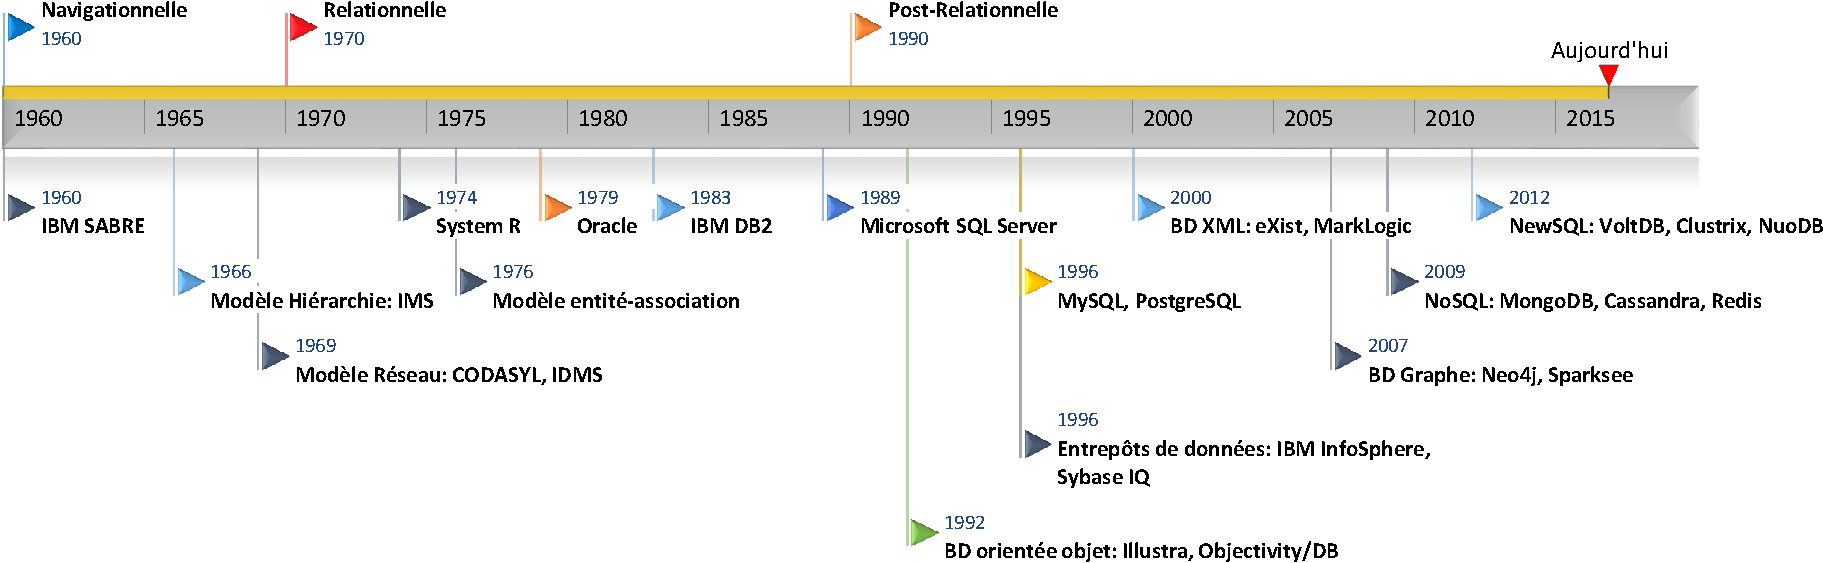
\includegraphics[scale=0.55]{chapitre2/chap2Fig/db-timeline.pdf}
\caption{Une brève évolution de la technologie des bases de données.}
 \label{fig:db-timeline}
\end{center}
\end{figure}

\subsection{Conception et cycle de vie}
% book: Database Systems - Design Implementation
% 1.4 WHY DATABASE DESIGN IS IMPORTANT

Une des tâches essentielles des développeurs de bases de données est la conception de leurs schémas. La conception de base de données est le processus de production d'un modèle de données détaillé de la base de données. Ce modèle de données contient tous les choix de conception logique et physique nécessaires et les paramètres de stockage physique nécessaires pour générer une conception dans un langage de définition de données, qui peut ensuite être utilisé pour créer une base de données. La représentation doit être juste pour éviter les erreurs sémantiques, notamment dans les réponses aux requêtes. Elle doit aussi être complète pour permettre le développement des programmes d’application souhaités. Elle doit enfin être évolutive afin de supporter la prise en compte rapide de nouvelles demandes \cite{Gardarin03}.

Une base de données bien conçue facilite la gestion des données et génère des informations précises et précieuses. Une base de données mal conçue est susceptible de devenir un terrain fertile pour les erreurs difficiles à tracer qui peuvent conduire à une mauvaise prise de décision et à l'échec d'une organisation. Même un bon SGBD fonctionnera mal avec une base de données mal conçue. La conception de base de données est tout simplement trop importante pour être laissée à la chance. L'objectif principal est de créer des modèles conceptuels, logiques et physiques complets, normalisés, non redondants et entièrement intégrés.

La création et l'évolution des bases de données suivent un schéma itératif appelé cycle de vie, un processus continu de création, de maintenance, d'amélioration et de remplacement des BDs. Traditionnellement, la démarche de conception et de cycle de vie d'une base de données s’effectue par des abstractions successives et itératives, en descendant depuis les problèmes de l’utilisateur vers la base de données finale \cite{Coronel09}. Nous proposons de distinguer cinq étapes :

% book: Physical Database Design
% 1.2 Database Life Cycle (p.26)
\begin{figure}
\begin{center}
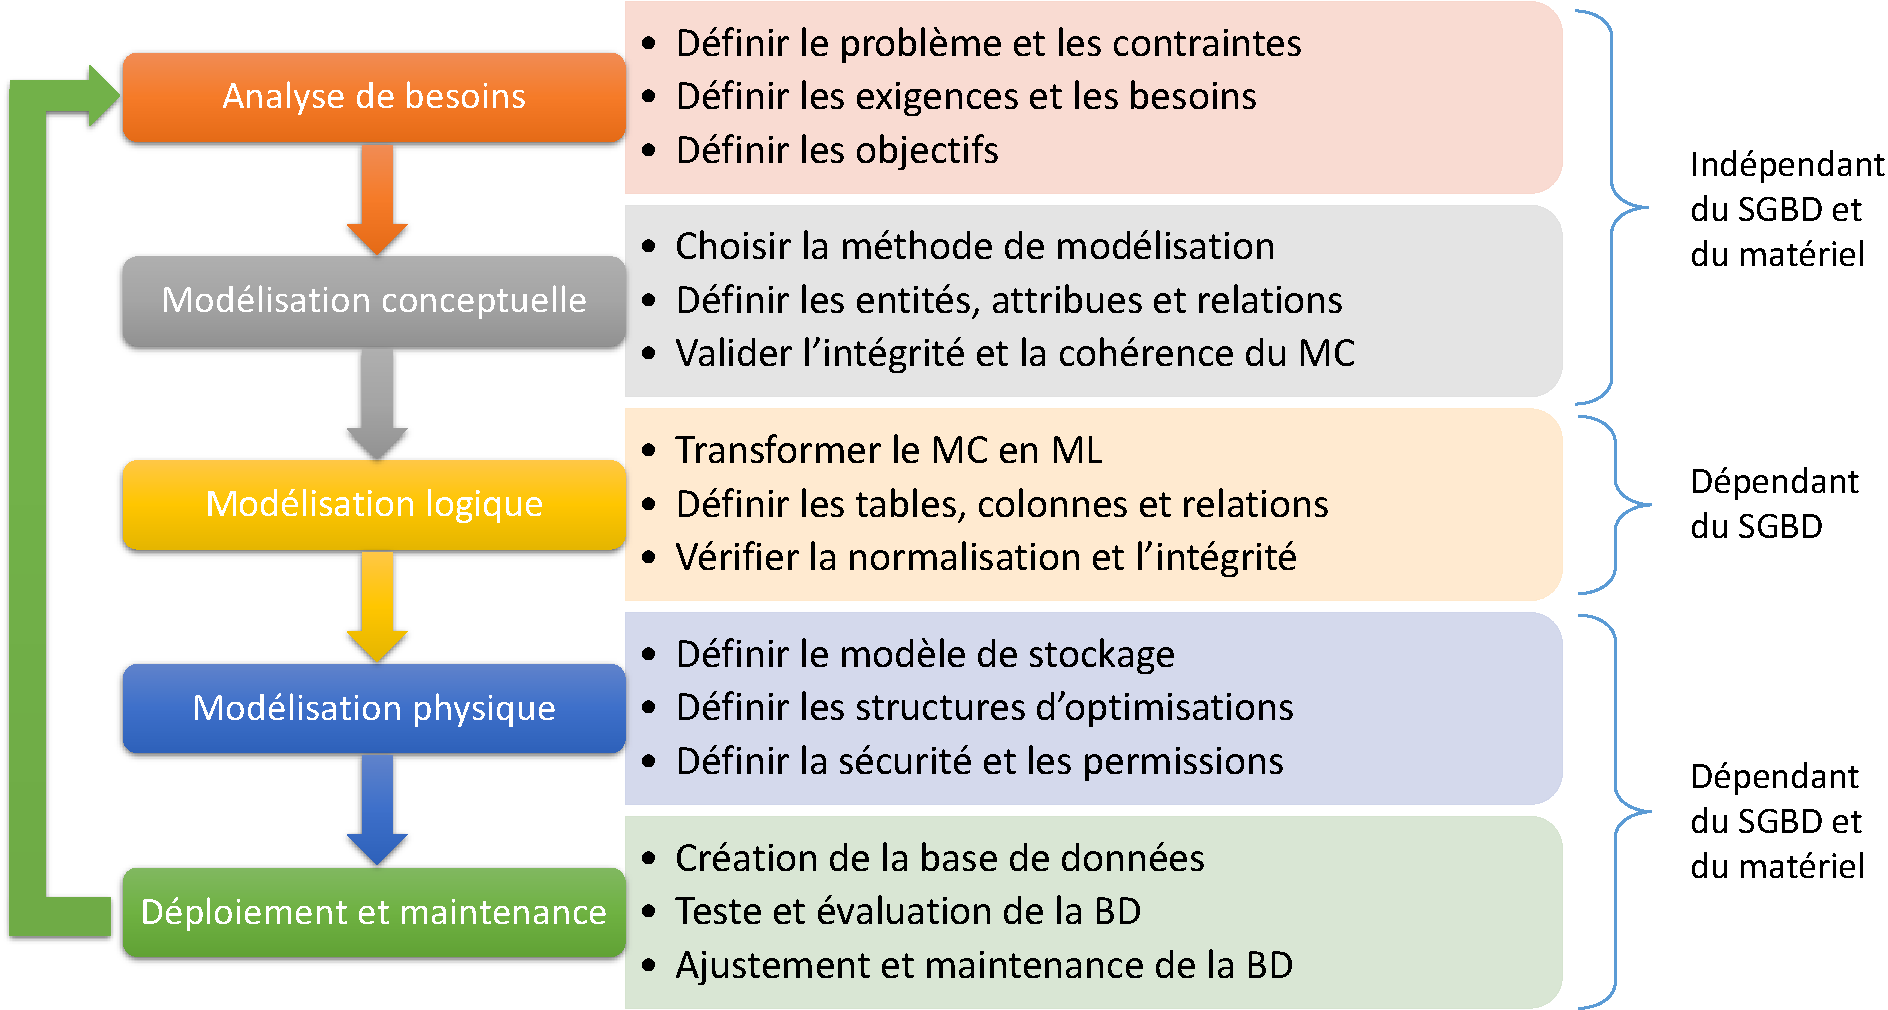
\includegraphics[scale=0.5]{chapitre2/chap2Fig/db-lifecycle.pdf}
\caption{Le cycle de vie des bases de données.}
 \label{fig:db-lifecycle}
\end{center}
\end{figure}

\begin{enumerate}
 \item \textbf{Analyse des besoins}. Consiste à définir et examiner les problèmes, les contraintes et les objectifs de l'entreprise. Une première évaluation des besoins et exigences, logiciels et matériels, relatives au flux d'information doit être effectuée lors de cette étape. La phase d'analyse du cycle de vie est, en fait, une vérification approfondie des besoins des utilisateurs. Le résultat est une spécification textuelle de ces besoins.
 \item \textbf{Modélisation conceptuelle}. L'objectif de cette étape est de concevoir une base de données indépendante du logiciel et des détails physiques de la base de données. La sortie de ce processus est un modèle de données conceptuelles qui décrit les principales entités de données, les attributs, les relations et les contraintes d'un domaine de problème donné. Cette conception est descriptive et narrative en forme. C'est-à-dire qu'elle est généralement composée d'une représentation graphique ainsi que de descriptions textuelles des principaux éléments de données, relations et contraintes. L'objectif est d'intégrer toutes les parties dans un schéma conceptuel global complet, non redondant et cohérent. Ce schéma global est développé en utilisant des techniques telles que la modélisation entité-association ou \gls{UML}.
 \item \textbf{Modélisation logique}. L'objectif de la modélisation logique est de concevoir une base de données à l'échelle de l'entreprise basée sur un modèle de données spécifique, mais indépendante des détails de niveau physique. La conception logique nécessite que tous les objets du modèle conceptuel soient mappés aux structures spécifiques utilisées par le modèle de base de données sélectionné. Par exemple, la conception logique d'un SGBD relationnel comprend les spécifications pour les relations (tables). Avec un SGBD objet, il s’agit de générer des classes et des associations. La conception logique ne doit contenir que des tables correctement normalisées et nécessite également la définition des domaines d'attributs et des contraintes appropriées.
 \item \textbf{Modélisation physique}. La modélisation ou conception physique est le processus de détermination de l'organisation du stockage de données et des caractéristiques d'accès aux données afin d'en assurer l'intégrité, la sécurité et les performances du système. Il s'agit de la dernière étape du processus de conception de base de données. Les caractéristiques de stockage sont déterminées en fonction des types de périphériques pris en charge par le matériel, du type de méthodes d'accès aux données prises en charge par le système et le SGBD. Dans cette étape, il faut choisir les bonnes structures d'optimisations physiques : vues matérialisées ou partitionnement de tables, index, etc. La conception physique pourrait devenir un travail très technique qui affecte non seulement l'accessibilité des données dans le(s) périphérique(s) de stockage, mais aussi la performance du système.
 \item \textbf{Déploiement et maintenance}. Le résultat des phases de conception de base de données est une série d'instructions détaillant la création de tables, d'attributs, d'index, de contraintes de sécurité, de règles de stockage, de performance, d'une architecture centralisée ou distribuée, etc. Dans cette phase, toutes ces spécifications de conception doivent être mises en œuvre. L'administrateur teste, évalue et ajuste la base de données pour s'assurer qu'elle fonctionne comme prévu. L'administrateur doit aussi effectuer des activités de maintenance dans la base de données. Certaines des activités de maintenance périodique comprennent la sauvegarde, la restauration, la modification des attributs et tables, génération de statistiques, audits de sécurité, etc.
\end{enumerate}

Le schéma illustré par la \ref{fig:db-lifecycle}, représente ce cycle de vie avec les tâches principales de chaque étape. Dans les sections suivantes nous détaillons ces différentes étapes en mettant l'accent sur la phase de conception physique.

\subsubsection{Analyse des besoins}
Dans le domaine de l'ingénierie logicielle, l'ingénierie des besoins est la branche du génie logiciel qui se consacre aux objectifs, aux fonctions et aux contraintes réels des systèmes logiciels. Elle s'intéresse également à la relation entre ces facteurs et les spécifications précises du comportement des logiciels, ainsi qu'à leur évolution dans le temps et dans les familles de logiciels \cite{Zave97}. Autrement dit, les besoins et les exigences des utilisateurs sont traduits en un ensemble de besoins qui définissent ce que le système doit faire et comment il doit le faire. Le concepteur de base de données doit s'assurer que les besoins sont compréhensibles, sans ambiguïté, complets et concis.
Les systèmes matériels et logiciels existants sont également étudiés pendant la phase d'analyse. Le résultat de l'analyse devrait être une meilleure compréhension des domaines fonctionnels du système et des problèmes actuels ou potentiels. Les utilisateurs finaux et le concepteur de systèmes doivent travailler ensemble pour identifier les processus et pour découvrir les zones à problèmes potentielles. Cette coopération est essentielle pour définir les objectifs de performance appropriés permettant de juger le nouveau système \cite{Coronel09}. Une bonne analyse des besoins est fondamentale pour une conception réussie de la base de données.
Les besoins se répartissent généralement en deux types: \textit{besoins fonctionnels} ($\mathcal{\acrshort[hyper=false]{BF}}$) et \textit{besoins non-fonctionnels} ($\mathcal{\acrshort[hyper=false]{BNF}}$) \cite{Zave97,Chung12,Ameller12}, tel que représenté dans la \ref{fig:reqs-classification}.

\paragraph{Besoin fonctionnel}
Le $\mathcal{BF}$ est défini comme étant tout besoin qui spécifie \textit{ce que} le système doit faire. En d'autres termes, un $\mathcal{BF}$ décrira un comportement particulier du fonctionnement du système lorsque certaines conditions sont valides, par exemple: << envoyer un courrier électronique lorsqu'un nouveau client s'inscrit >>. Des exemples des BFs dans une base de données incluent : gestion de transactions, authentification, niveaux d'autorisation, exigences de certification, données historiques, exigences légales ou réglementaires, etc.

\paragraph{Besoin non-fonctionnel}
Le $\mathcal{BNF}$ est défini comme étant tout besoin qui spécifie \textit{comment} le système effectue une certaine fonction. En d'autres termes, un $\mathcal{BNF}$ décrira comment un système doit se comporter et quelles limites il y a sur sa fonctionnalité. Les BNFs spécifient généralement les attributs ou caractéristiques de qualité du système, par exemple: << les données modifiées dans une base de données doivent être mises à jour pour tous les utilisateurs qui y accèdent en moins de 2 secondes >>. Par exemple, citons : performance, temps de réponse, consommation d'énergie,  évolutivité, disponibilité, fiabilité, la sécurité, utilisabilité, etc. Les BNFs sont généralement plus difficiles à analyser. En particulier, les BNFs ont tendance à être des propriétés d'un système dans son ensemble et ne peuvent donc pas être vérifiés pour des composants individuels \cite{Nuseibeh00}.

En outre, les BNFs peuvent être classés en deux catégories : $\mathcal{BNF}$ mesurable (BNFM) et $\mathcal{BNF}$ non-mesurable (BNFNM) \cite{Siegmund08}.

\subparagraph{BNFM}
Les BNFM sont des besoins qui peuvent être mesurés sur une échelle métrique définie par l'utilisateur. La métrique est définie par l'utilisateur car pour certains besoins, tel que la performance, il existe plusieurs métriques pour la quantifier. Les mesures peuvent être réalisées automatiquement par un ordinateur comme le temps de réponse, ou manuellement par un dispositif de mesure comme la consommation d'énergie.

\subparagraph{BNFNM}
Cette classe contient des besoins qui ne peuvent être décrits que qualitativement à l'aide d'une échelle ordinaire ou nominale, c'est-à-dire qu'il n'existe aucune métrique à partir de laquelle nous pouvons extraire des mesures quantifiables. Par exemple, considérer l'utilisabilité. Il faut réaliser de grandes études aux niveau des utilisateurs du système pour quantifier l'influence de différentes caractéristiques sur l'utilisabilité du système. L'évaluation d'une telle étude se fait d'habitude manuellement.

\begin{figure}
\footnotesize
\begin{center}
\tikzset{
  basic/.style  = {draw, text width=8em, drop shadow, rectangle},
  root/.style   = {basic, rounded corners=2pt, thin, align=center,
                   fill=green!30},
  level 1/.style = {basic, rounded corners=6pt, thin,align=center, fill=green!60,
                   text width=8em,sibling distance=55mm},
  level 2/.style = {basic, rounded corners=6pt, thin,align=center, fill=green!60,
                   text width=8em,sibling distance=40mm},
  level 3/.style = {basic, thin, align=left, fill=pink!60, text width=6.5em}
}
\begin{tikzpicture}[
  edge from parent/.style={->,draw,black},
  >=latex]

% root of the the initial tree, level 1
\node[root] {Types de besoins}
% The first level, as children of the initial tree
  child {node[level 1] (c1) {Fonctionnel}}
  child {node[level 1] (c2) {Non-fonctionnel}
	child {node[level 2] (c3) {Mesurable}}
	child {node[level 2] (c4) {Non-Mesurable}}
  };
  
\begin{scope}[every node/.style={level 3}]
\node [below of = c1, xshift=5pt] (c11) {Niveaux d'autorisations};
\node [below of = c11] (c12) {$\cdots$};
\node [below of = c3, xshift=5pt] (c31) {Performance};
\node [below of = c31] (c32) {$\cdots$};
\node [below of = c4, xshift=5pt] (c41) {Utilisabilité};
\node [below of = c41] (c42) {$\cdots$};
\end{scope}

\foreach \value in {1,...,2}
  \draw[->] (c1.178) |- (c1\value.west);
  
\foreach \value in {1,...,2}
  \draw[->] (c3.178) |- (c3\value.west);
  
\foreach \value in {1,...,2}
  \draw[->] (c4.178) |- (c4\value.west);

\end{tikzpicture}
\caption{Classification des types de besoins.}
\label{fig:reqs-classification}
\end{center}
\end{figure}

% book: Bases de données
% conception des bd p661
% 2. MODÉLISATION DES DONNÉES p15

% book: Database Systems - Design Implementation
% chapter 9: database design

% eBISS 2016
% 5 Audit of the DW Life Cycle
\subsubsection{Modélisation conceptuelle}
La modélisation conceptuelle consiste à créer un schéma conceptuel pour la base de données, à partir des besoins déjà collectés et analysés, en utilisant un modèle de données conceptuelles de haut niveau, tel que le modèle entité-association ou digramme de classe UML. Ce schéma représente les objets du monde réel de la manière la plus réaliste possible. Le modèle conceptuel doit comprendre une compréhension claire de l'entreprise et de ses $\mathcal{BF}$ et $\mathcal{BNF}$. À ce niveau d'abstraction, le type de matériel et/ou de SGBD à utiliser pourrait ne pas avoir été identifié. Par conséquent, la conception doit être indépendante du logiciel et du matériel afin que le système puisse être installé dans n'importe quelle plate-forme matérielle et logicielle choisie plus tard \cite{Coronel09}.

\begin{example}
 Une société spécialisée dans la vente souhaite dynamiser sa politique de vente en construisant un site web pour la vente de ses produits. Après l'étude des besoins de l'entreprise, le concepteur de BD a créé un schéma conceptuel avec le modèle entité-association. Voici la description de chaque entité :
 \begin{itemize}
  \item \textit{Clients} : Cette table conserve les informations sur les clients.
  \item \textit{Commandes} : Contient la liste des commandes des clients.
  \item \textit{Détail commandes} : Contient les informations détaillées sur les commandes.
  \item \textit{Produits} : Garde la liste des produits avec leur détaille.
  \item \textit{Stock} : Sauvegarde la quantité de chaque produit en stock.
 \end{itemize}
 Un exemple de schéma conceptuel défini en termes d'entités et d'associations entre ces entités est représenté dans la \ref{fig:conceptual-design-ex}.
\end{example}

\begin{figure}
\begin{center}
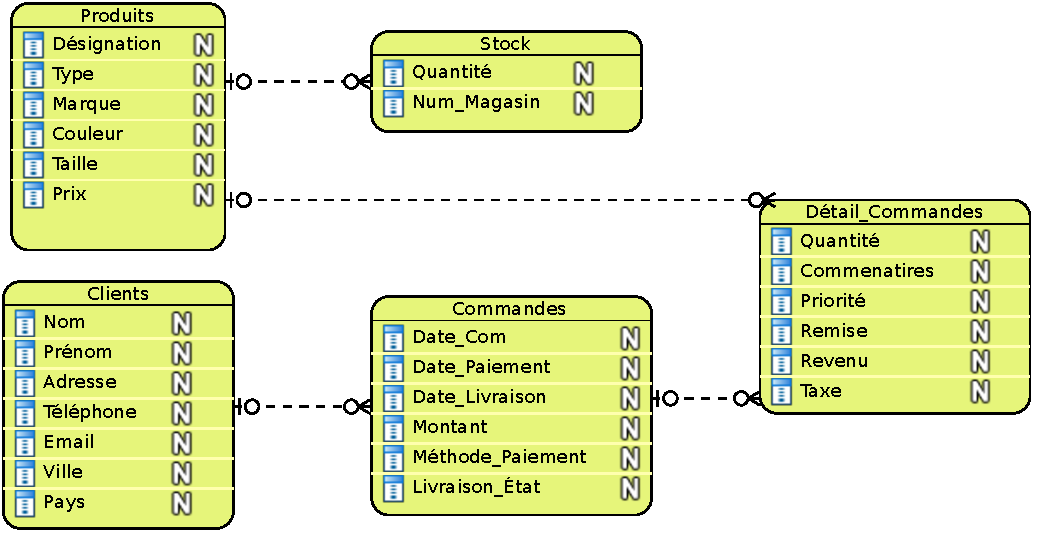
\includegraphics[scale=0.6]{chapitre2/chap2Fig/conceptual-design-ex.pdf}
\caption{Exemple d'un schéma de modélisation conceptuelle.}
\label{fig:conceptual-design-ex}
\end{center}
\end{figure}

\subsubsection{Modélisation logique}
La modélisation logique commence par le choix du SGBD suivant le modèle de données choisi dans l'étape précédente. Ensuite, le schéma conceptuel est transformé du modèle de données de haut niveau en modèle de données de mise en œuvre avec le SGBD \cite{Elmasri08}.
La création schéma logique peut se faire d'une manière automatisée. Il existe des règles sur la façon dont le modèle entité-association ou le diagramme de classe UML est transféré à des relations du schéma logique. Dans cette étape, les clés primaires et les clés étrangères sont définies.
La normalisation est la dernière partie de la conception logique. L'objectif de la normalisation est d'éliminer la redondance et les anomalies potentielles lors de la mise à jour. La redondance signifie que les mêmes données sont enregistrées plus d'une fois dans la base de données. L'anomalie de mise à jour est une conséquence de la redondance. Si une donnée est enregistrée en plusieurs endroits, les mêmes données doivent être mises à jour en plusieurs endroits. La normalisation est une technique par laquelle on peut modifier le schéma relationnel pour réduire la redondance \cite{Elmasri08}.

\begin{figure}
\begin{center}
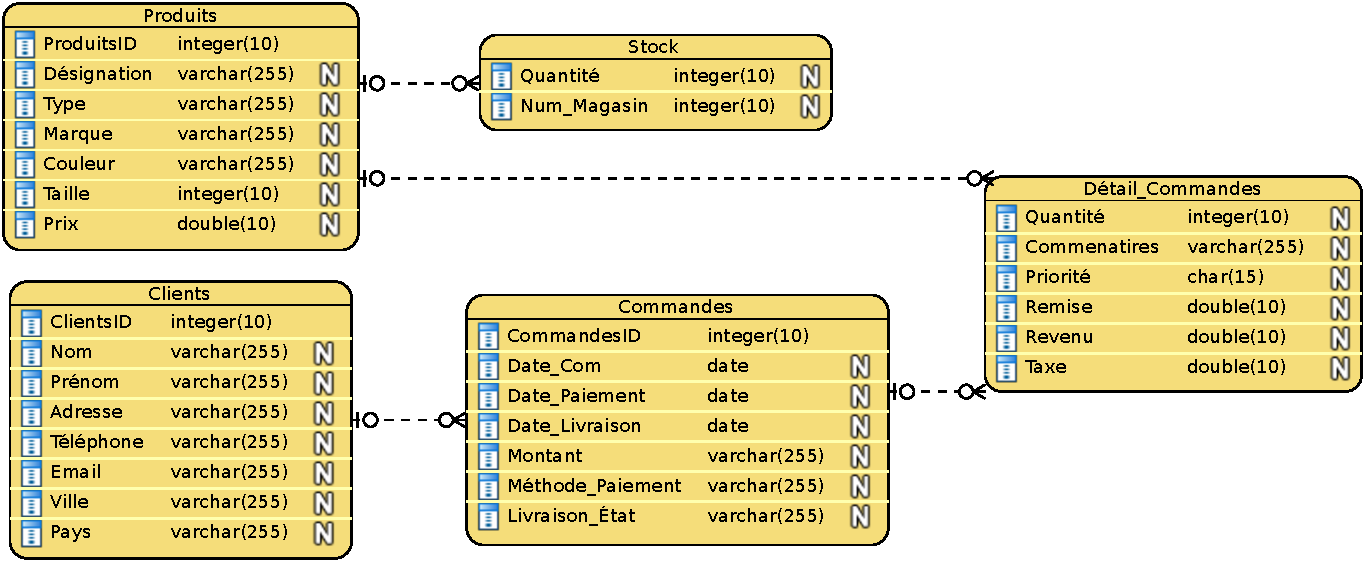
\includegraphics[scale=0.6]{chapitre2/chap2Fig/logical-design-ex.pdf}
\caption{Exemple d'un schéma de modélisation logique.}
\label{fig:logical-design-ex}
\end{center}
\end{figure}

\begin{example}
La \ref{fig:logical-design-ex} représente le schéma logique de notre exemple de gestion de vente. En peut remarquer que la définition des types de données des attributs et les clés primaires ont été établies sur les tables << \textit{Stock} >>, << \textit{Commandes} >> et << \textit{Clients} >>.
\end{example}

\subsubsection{Modélisation physique}
L'étape suivante est la conception physique, au cours de laquelle les structures de stockage internes, les organisations de fichiers, les indexes, les chemins d'accès, les contraintes d'intégrité, les droits d'accès des utilisateurs et les paramètres de conception physique des fichiers de base de données sont spécifiés \cite{Elmasri08}.

Dans cette étape, des structures d'optimisation ($\mathcal{\acrshort[hyper=false]{SO}}$) telles que les vues matérialisées, les indexes, le partitionnement de données, sont sélectionnées pour optimiser un ou plusieurs $\mathcal{BNF}$ tels que la performance des requêtes et l'énergie du système. La conception physique se concentre sur les méthodes de stockage et d'accès aux tables sur le disque qui permettent à la base de données de fonctionner avec une efficacité élevée. L'objectif est de maximiser les performances de la base de données sur l'ensemble du système. Les ressources physiques qui impliquent les performances lors de l'exécution des requêtes comprennent le CPU, les E/S (par exemple, les disques) et les connexions réseaux \cite{Lightstone10}.

\begin{example}
La \ref{fig:physical-design-ex} illustre le schéma physique de l'exemple précédent. Les informations ajoutées sont les clés étrangères sur les tables << \textit{Stock} >>, << \textit{Commandes} >> et << \textit{Détail\_Commandes} >>, et les indexes définis sur les tables << \textit{Clients} >> et << \textit{Produits} >> pour accélérer l'accès aux données de ces tables.\end{example}

\begin{figure}
\begin{center}
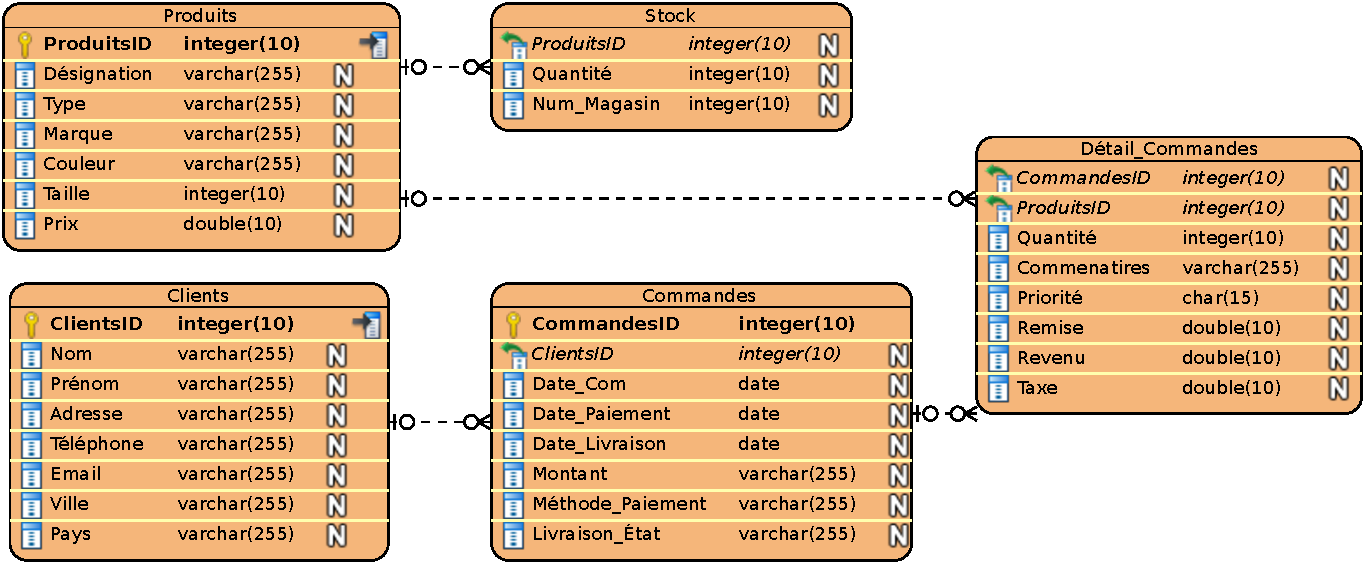
\includegraphics[scale=0.6]{chapitre2/chap2Fig/physical-design-ex.pdf}
\caption{Exemple d'un schéma de modélisation physique.}
\label{fig:physical-design-ex}
\end{center}
\end{figure}

Les optimisations physiques ont été amplifiées par l'explosion du volume des données et la nécessité d'optimiser ses modèles d'accès, ce qui est assuré par les $\mathcal{SO}$ \cite{ChaudhuriN07}. En exploitant les $\mathcal{SO}$, on peut réduire le temps de traitement des opérations dans certains cas de plusieurs ordres de grandeur. Une tâche critique pour l'administrateur de la base de données dans cette phase est le bon choix des $\mathcal{SO}$ pour satisfaire les $\mathcal{BNF}$ des utilisateurs. Cette tâche peut être divisée en quatre sous-tâches \cite{BellatrecheHdr09} :

\begin{enumerate}
 \item Le choix des structures d’optimisation : redondante ou non-redondante;
 \item Le choix du mode de sélection des structures d'optimisation : isolée ou multiple;
 \item Le choix et le développement des algorithmes de résolution;
 \item La validation et le déploiement des solutions d’optimisation.
\end{enumerate}

Dans ce suit, nous considérons le cas des vues matérialisées ($\mathcal{\acrshort[hyper=false]{VM}}$) qui est une $\mathcal{SO}$ redondante très utilisé dans les applications décisionnelles et les requêtes de type OLAP. 
% these kamel boukhelfa, ahcene
%\paragraph{Structure d'optimisation : Définition et classification}
\paragraph{Cas d'étude : Vues matérialisées}\label{sec:psv}
\begin{definition}
 Une vue est une relation logique qui utilise la définition de requête pour extraire les données à partir des tables correspondantes.
\end{definition}

\begin{definition}
 Une vue matérialisée est une table sur disque qui contient les résultats d'une requête. Elle peut s'agir d'une copie locale de données située à distance, ou un sous-ensemble des lignes et/ou colonnes d'un résultat de requête ou de jointure avec ou sans une fonction d'agrégation.
\end{definition}

Les $\mathcal{VM}$ sont de petites tailles par rapport à la table réelle et sont constituées de données importantes. Par conséquent, une exécution plus rapide des requêtes est possible. Lorsque les requêtes sont générées dans le système, les $\mathcal{VM}$ sont accédées en premier. Si les résultats ne sont pas trouvés dans les $\mathcal{VM}$, les tables réelles du système sont recherchées.

\begin{example}
Pour créer une vue matérialisée qui comptabilise la somme des ventes de chaque client par jour de notre base de données de vente, la requête SQL s'écrit comme suit :
	%\begin{verbatim}
	\begin{lstlisting}[language=Sql]
	CREATE MATERIALIZED VIEW resume_ventes AS
	SELECT Nom, Date_Com, SUM(Montant)
	FROM Clients Commandes
	WHERE Clients.ClientsID = Commandes.ClientsID
	GROUP BY Nom, Date_Com
	ORDER BY Nom, Date_Com;
    \end{lstlisting}
	%\end{verbatim}
Si la relation \textit{Commandes} contient des dizaines de millions de tuples, la différence entre le calcul de l'agrégation à partir des données de base et à l'aide de la vue matérialisée peut être de plusieurs ordres de grandeur.
\end{example}


Les défis à relever pour exploiter les vues matérialisées sont : (1) identifier les bonnes vues à matérialiser, (2) exploiter les $\mathcal{VM}$ pour répondre aux requêtes, et (3) mettre à jour efficacement les $\mathcal{VM}$ lors du changement des données de base \cite{Chaudhuri97b}.

\subparagraph{Problème de sélection des $\mathcal{VM}$}

L'administrateur de base de données ne peut pas matérialiser toutes les vues possibles, car il est limité par certaines ressources comme, l'espace disque et le temps de calcul, ceci est connu comme le problème de sélection des vues matérialisées ($\mathcal{\acrshort[hyper=false]{PSV}}$).
Le $\mathcal{PSV}$ consiste à trouver un ensemble approprié de vues satisfaisant un ensemble donné de $\mathcal{BNF}$ tels que la performance des requêtes, la fiabilité, l'utilisabilité, etc. Les $\mathcal{VM}$ sélectionnées doivent répondre à un ensemble de contraintes telles que le coût de stockage, les coûts de maintenance, etc. Le $\mathcal{PSV}$ est connu pour être un problème NP-complet \cite{Gupta99} en raison du fait que l'espace de solution s'accroît de façon exponentielle lorsque la taille du problème augmente. La formalisation générale de $\mathcal{PSV}$ est défini comme suit : Étant donné :

\begin{itemize}
\item un schéma d'une base de données : $DB$; 
\item une charge de requêtes : $\mathcal{W} = \{Q_1, Q_2, \cdots , Q_n\}$; 
\item un ensemble de contraintes : $\mathcal{C} = \{C_1, C_2, \cdots$ $ , C_p\}$; 
\item un ensemble de besoins non-fonctionnelles : $\mathcal{BNF} = \{nfr_1,$ $\cdots, nfr_k\}$. 
\end{itemize}

Le $\mathcal{PSV}$ consiste à sélectionner un ensemble de vues matérialisées : $MV = \{V_1, V_2, \cdots , V_m\}$ satisfaisant des $\mathcal{BNF}$ et en respectant l'ensemble des contraintes $\mathcal{C}$.

\begin{figure}
	\centering
	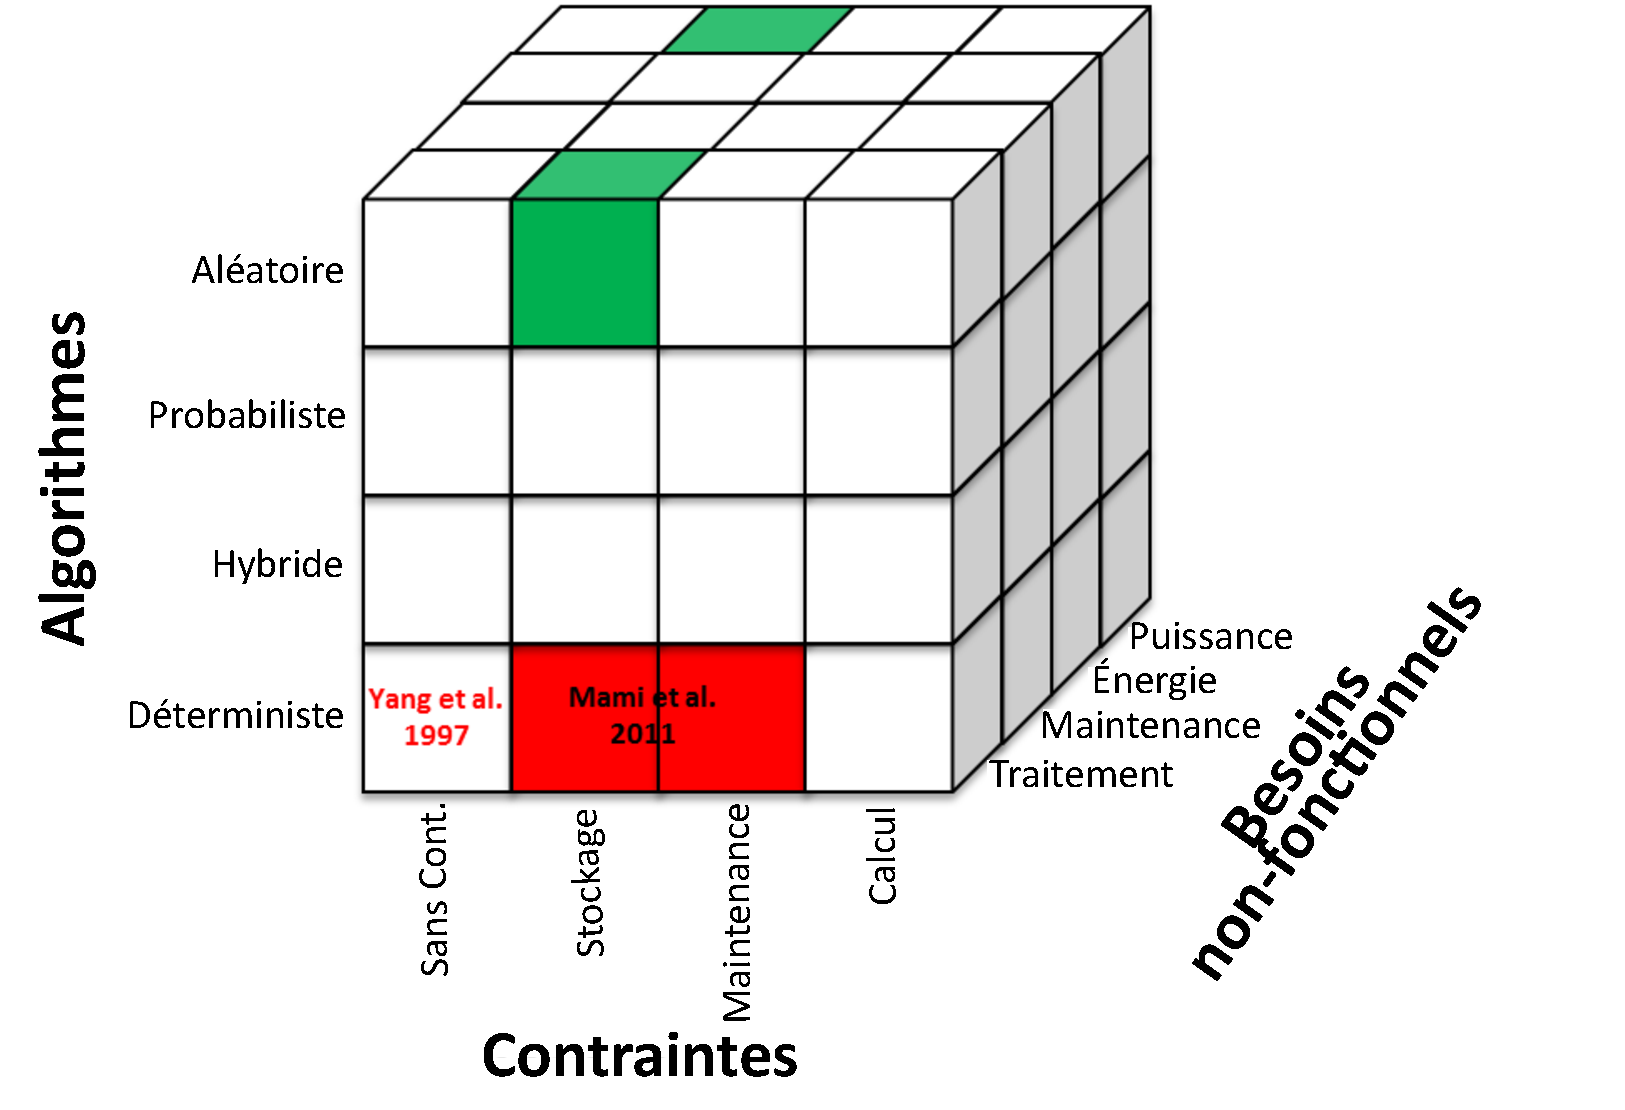
\includegraphics[scale=0.4]{chapitre2/chap2Fig/cubeNFR.pdf}
	\caption{Méthodes de résolutions du $\mathcal{PSV}$ .}
	\label{fig:warehouse-solutions}
\end{figure}

Plusieurs instanciations de cette formalisation existent. Nous proposons de les représenter par un \textit{cube} ayant trois dimensions principales : (i) le $\mathcal{BNF}$, (ii) les contraintes $\mathcal{C}$, et (iii) les algorithmes utilisés pour résoudre le $\mathcal{PSV}$. Ces dimensions permettent de classer les solutions existant dans l'état de l'art. La \ref{fig:warehouse-solutions} illustre notre cube.

\textbf{Les $\mathcal{BNF}$.} En ce qui concerne les $\mathcal{BNF}$ que les $\mathcal{VM}$ sélectionnés doivent satisfaire, elles couvrent plusieurs objectifs, tels que : la minimisation du temps de réponse des requêtes \cite{Ross96}, la minimisation du temps de réponse et du coût de maintenance \cite{Gupta97}. Ces objectifs peuvent être combinés pour donner lieu à une formalisation \textit{multi-objectif} du $\mathcal{PSV}$ comme dans \cite{Lawrence06} où le temps de réponse et le coût de maintenance ont été considérés.

\textbf{Les contraintes.} Les premières études sur le $\mathcal{PSV}$ supposent l'absence de contraintes \cite{Mistry01}. Par la suite et en raison de la grande taille de stockage des $\mathcal{VM}$ sélectionnées, l'espace de stockage devient la principale contrainte que le processus de sélection doit intégrer \cite{Gupta97}. Ensuite, le coût de maintenance devient un paramètre important car les $\mathcal{VM}$ sélectionnées doivent être mises à jour une fois les tables de base modifiées \cite{Gupta99}. Certaines études ont considéré les deux contraintes \cite{Kalnis02}. Récemment, des études traitent le cas du déploiement des $\mathcal{VM}$ dans un environnement distribué avec le coût de communication réseaux comme contrainte \cite{Chaves09,Mami16}, ou encore un environnement cloud sous la contrainte de coût monétaire \cite{Kehua14}. 

\textbf{Algorithmes de résolution.} 
La résolution de $\mathcal{PSV}$ est généralement réalisée soit par des algorithmes simples ou avancés qui couvrent des algorithmes \textit{déterministes} \cite{Gupta99,Gupta97,Boukorca15}, algorithmes \textit{aléatoires} \cite{Kalnis02,Lawrence06}, algorithmes \textit{hybrides} \cite{Zhang01}, et la \textit{programmation par contraintes} \cite{Mami11,Mami16} (pour plus de détails, voir l'étude de \cite{Mami12,Chirkova11}).

\textbf{Type de sélection.} Il existe deux approches pour la sélection des vues : \textit{statique} et \textit{dynamique}. Une approche de sélection de vue statique suppose que la charge de requêtes est fixe, et choisit ensuite l'ensemble de vues à matérialiser \cite{Yang97,Boukorca15}. Alors que, dans une approche de sélection de vue dynamique, la sélection est appliquée lorsqu'une requête arrive. Par conséquent, la charge de requêtes est construite progressivement et change avec le temps \cite{Kehua14,Kotidis99}.

\textbf{Structure de données.} Habituellement, la première étape dans la résolution de $\mathcal{PSV}$ est l'identification des vues candidates qui sont prometteuses pour la matérialisation. De nombreuses techniques de structures de données ont été proposées pour obtenir l'ensemble des vues candidates \cite{Mami12}:
\begin{itemize}
 \item \textbf{\textit{Graphe de vue ET/OU}} : est un graphe orienté acyclique (\acrshort[hyper=false]{DAG}), composé de deux types de nœuds : opération et équivalence. Chaque nœud d'opération correspond à une opération algébrique dans le plan d'une requête (sélection, jointure, projection, etc.). Chaque nœud d'équivalence correspond à un ensemble d'expressions logiques équivalentes. De nombreux algorithmes ont été proposés dans la littérature exploitant cette structure \cite{Gupta99,Gupta97,Mami11}. La \ref{fig:dag-andor-example} donne un exemple de graphe de vue ET/OU.
 \item \textbf{\textit{Traitement de plan multi-vue (\acrshort[hyper=false]{MVPP})}} : Le MVPP défini par Yang \textit{et al} \cite{Yang97} est un DAG dans lequel les nœuds racine sont les requêtes, les nœuds feuilles sont les relations de base et tous les autres nœuds intermédiaires sont des vues de sélection, de projection, de jointure ou d'agrégation qui contribuent à la construction d'une requête donnée \cite{Boukorca15,Zhang01}. Un exemple d'un MVPP est représenté sur la \ref{fig:dag-mvpp-example}.
 \item \textbf{\textit{Données cube treillis}} : est un DAG proposé dans le contexte des entrepôts de données multidimensionnel, dont les nœuds représentent les requêtes ou vues qui sont caractérisées par une opération de regroupement, et les arêtes définissent la relation entre les vues \cite{Kalnis02,Harinarayan96,Yu03}. La \ref{fig:dag-cubelattice-example} donne un exemple du graphe de treillis.
 \item \textbf{\textit{Transformation de requête}} : dans cette technique, le $\mathcal{PSV}$ prend comme entrer les définitions de requête. Le $\mathcal{PSV}$ est modélisé comme un problème de recherche d'espaces d'états en utilisant un ensemble de règles de transformation. Ces règles détectent et exploitent des sous-expressions communes entre les requêtes de la charge et garantissent que toutes les requêtes peuvent être répondu en utilisant exclusivement les $\mathcal{VM}$ \cite{Ligoudistianos98,Theodoratos97}.
 \item \textbf{\textit{Analyse syntaxique}} : cette technique analyse la charge de requêtes et sélectionne un sous-ensemble de relations à partir duquel on peut matérialiser une ou plusieurs vues, à condition de réduire le coût de la charge de requêtes de manière significative \cite{Agrawal00,Chaves09}.
\end{itemize}

\begin{figure}
  \centering
  \subfloat[Exemple d'un graphe de vue ET/OU.\label{fig:dag-andor-example}]{
    \resizebox{.3\textwidth}{!}{% \documentclass{standalone}
% \usepackage{tikz}
% \begin{document}
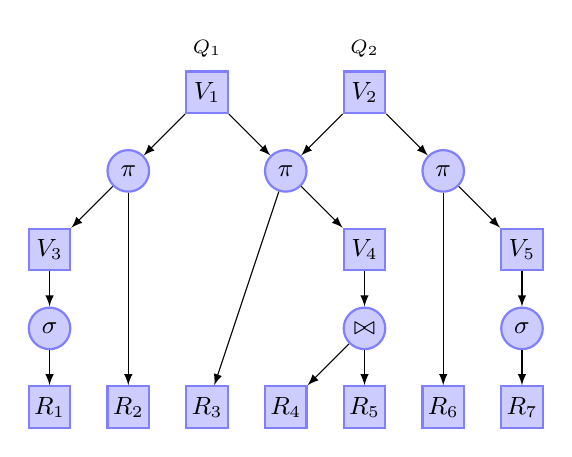
\begin{tikzpicture}[
every node/.style  = {fill=blue!20,draw=blue!50,thick,
	minimum size=1.5em,inner sep=0pt,font=\small},
circle_node/.style={circle},
rec_node/.style={rectangle},
edge from parent/.style={->,draw},
every label/.append style={font=\scriptsize},
>=latex]
  
    \node[rec_node] (r1) at (0, 0) {$R_1$};
    \node[rec_node] (r2) at (1, 0)  {$R_2$};
    \node[rec_node] (r3) at (2, 0) {$R_3$};
	\node[rec_node] (r4) at (3, 0) {$R_4$};
	\node[rec_node] (r5) at (4, 0) {$R_5$};
	\node[rec_node] (r6) at (5, 0) {$R_6$};
	\node[rec_node] (r7) at (6, 0) {$R_7$};
	
	\node[circle_node] (op1) at (0, 1) {$\sigma$};
	\node[circle_node] (op2) at (4, 1) {$\bowtie$};
	\node[circle_node] (op3) at (6, 1) {$\sigma$};
	
	\node[rec_node] (v3) at (0, 2) {$V_3$};
	\node[rec_node] (v4) at (4, 2) {$V_4$};
	\node[rec_node] (v5) at (6, 2) {$V_5$};
	
	\node[circle_node] (op4) at (1, 3) {$\pi$};
	\node[circle_node] (op5) at (3, 3) {$\pi$};
	\node[circle_node] (op6) at (5, 3) {$\pi$};
	
	\node[rec_node,label={\scriptsize $Q_1$}] (v1) at (2, 4) {$V_1$};
	\node[rec_node,label={\scriptsize $Q_2$}] (v2) at (4, 4) {$V_2$};


    \draw[->] (v1) -- (op4);
	\draw[->] (v1) -- (op5);
	\draw[->] (v2) -- (op5);
	\draw[->] (v2) -- (op6);
	
	\draw[->] (op4) -- (v3);
	\draw[->] (op4) -- (r2);
	\draw[->] (op5) -- (v4);
	\draw[->] (op5) -- (r3);
	\draw[->] (op6) -- (v5);
	\draw[->] (op6) -- (r6);
	
	\draw[->] (v3) -- (op1);
	\draw[->] (v4) -- (op2);
	\draw[->] (v5) -- (op3);
	
	\draw[->] (op1) -- (r1);
	\draw[->] (op2) -- (r4);
	\draw[->] (op2) -- (r5);
	\draw[->] (op3) -- (r7);
	
\end{tikzpicture}
%\end{document}
}
  }
  \quad
  \subfloat[Exemple d'un graphe de données cube treillis.\label{fig:dag-cubelattice-example}]{
    \resizebox{.15\textwidth}{!}{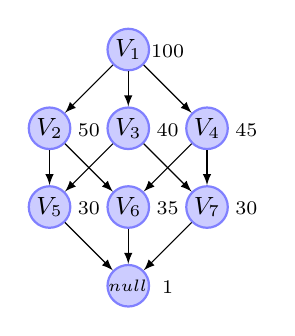
\begin{tikzpicture}[main_node/.style={circle,fill=blue!20,draw=blue!50,thick,
	minimum size=1.5em,inner sep=0pt,font=\small},
edge from parent/.style={->,draw},>=latex]
  
    \node[main_node,label={[shift={(0.5,-0.5)}]{\scriptsize 40}}] (1) at (0, 0) {$V_3$};
    \node[main_node,label={[shift={(0.5,-0.5)}]{\scriptsize 45}}] (2) at (1, 0)  {$V_4$};
    \node[main_node,label={[shift={(0.5,-0.5)}]{\scriptsize 50}}] (3) at (-1, 0) {$V_2$};
	\node[main_node,label={[shift={(0.5,-0.5)}]{\scriptsize 35}}] (4) at (0, -1) {$V_6$};
	\node[main_node,label={[shift={(0.5,-0.5)}]{\scriptsize 30}}] (5) at (1, -1) {$V_7$};
	\node[main_node,label={[shift={(0.5,-0.5)}]{\scriptsize 30}}] (6) at (-1, -1) {$V_5$};
	\node[main_node,label={[shift={(0.5,-0.5)}]{\scriptsize 100}}] (7) at (0, 1) {$V_1$};
	\node[main_node,label={[shift={(0.5,-0.5)}]{\scriptsize 1}}] (8) at (0, -2) {$_{null}$};

    \draw[->] (7) -- (3);
	\draw (7) edge[->] (2);
	\draw (3) edge[->] (4);
	\draw (2) edge[->] (4);
	
	\draw (1) edge[->] (6);
	\draw (1) edge[->] (5);
	\draw (6) edge[->] (8);
	\draw (5) edge[->] (8);
	
	\draw (7) edge[->] (1);
	\draw (3) edge[->] (6);
	\draw (4) edge[->] (8);
	\draw (2) edge[->] (5);
\end{tikzpicture}}
  }
  \quad
  \subfloat[Exemple d'un graphe de traitement de plan multi-vue.\label{fig:dag-mvpp-example}]{
    \resizebox{.35\textwidth}{!}{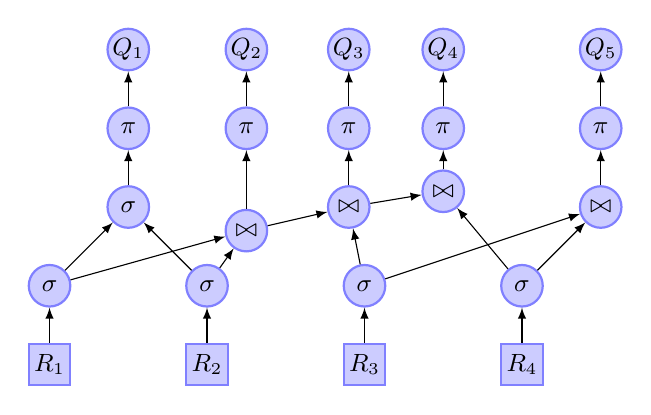
\begin{tikzpicture}[
every node/.style  = {fill=blue!20,draw=blue!50,thick,
	minimum size=1.5em,inner sep=0pt,font=\small},
circle_node/.style={circle},
rec_node/.style={rectangle},
edge from parent/.style={->,draw},
every label/.append style={font=\scriptsize},
>=latex]
  
    \node[rec_node] (r1) at (0, 0) {$R_1$};
    \node[rec_node] (r2) at (2, 0)  {$R_2$};
    \node[rec_node] (r3) at (4, 0) {$R_3$};
	\node[rec_node] (r4) at (6, 0) {$R_4$};
	
	\node[circle_node] (op1) at (0, 1) {$\sigma$};
	\node[circle_node] (op2) at (2, 1) {$\sigma$};
	\node[circle_node] (op3) at (4, 1) {$\sigma$};
	\node[circle_node] (op4) at (6, 1) {$\sigma$};
	
	\node[circle_node] (op5) at (1, 2) {$\sigma$};
	\node[circle_node] (op6) at (2.5, 1.7) {$\bowtie$};
	\node[circle_node] (op7) at (3.8, 2) {$\bowtie$};
	\node[circle_node] (op8) at (5, 2.2) {$\bowtie$};
	\node[circle_node] (op9) at (7, 2) {$\bowtie$};
	
	\node[circle_node] (op10) at (1, 3) {$\pi$};
	\node[circle_node] (op11) at (2.5, 3) {$\pi$};
	\node[circle_node] (op12) at (3.8, 3) {$\pi$};
	\node[circle_node] (op13) at (5, 3) {$\pi$};
	\node[circle_node] (op14) at (7, 3) {$\pi$};
	
	\node[circle_node] (q1) at (1, 4) {$Q_1$};
	\node[circle_node] (q2) at (2.5, 4) {$Q_2$};
	\node[circle_node] (q3) at (3.8, 4) {$Q_3$};
	\node[circle_node] (q4) at (5, 4) {$Q_4$};
	\node[circle_node] (q5) at (7, 4) {$Q_5$};

    \draw[->] (r1) -- (op1);
	\draw[->] (r2) -- (op2);
	\draw[->] (r3) -- (op3);
	\draw[->] (r4) -- (op4);
	
	\draw[->] (op1) -- (op5);
	\draw[->] (op1) -- (op6);
	\draw[->] (op2) -- (op5);
	\draw[->] (op2) -- (op6);
	\draw[->] (op3) -- (op7);
	\draw[->] (op3) -- (op9);
	\draw[->] (op4) -- (op8);
	\draw[->] (op4) -- (op9);
	
	\draw[->] (op5) -- (op10);
	\draw[->] (op6) -- (op11);
	\draw[->] (op6) -- (op7);
	\draw[->] (op7) -- (op12);
	\draw[->] (op7) -- (op8);
	\draw[->] (op8) -- (op13);
	\draw[->] (op9) -- (op14);
	
	\draw[->] (op10) -- (q1);
	\draw[->] (op11) -- (q2);
	\draw[->] (op12) -- (q3);
	\draw[->] (op13) -- (q4);
	\draw[->] (op14) -- (q5);
	
\end{tikzpicture}}
  }
  \caption{Des exemples de structures de données graphe orienté acyclique.}\label{fig:dag-examples}
\end{figure}

\subparagraph{Problème d'exploitation des $\mathcal{VM}$}
Le problème d'exploitation des $\mathcal{VM}$ est de trouver des méthodes efficaces pour répondre à une requête en utilisant un ensemble de $\mathcal{VM}$ précédemment définies sur la base de données, plutôt que d'accéder aux relations de base de données, afin d'améliorer le temps de traitement des requêtes \cite{Halevy01}. Cela se fait à l'aide de la \textit{réécriture de requête} : l'objectif est de trouver une réécriture équivalente de la requête originale en utilisant une ou plusieurs vues. Ce problème est prouvé NP-complet \cite{Levy95}.

Les approches proposées dans la littérature pour résoudre ce problème se basent sur l'adaptation du modèle de coût de l'optimiseur de requêtes afin de générer le meilleur plan équivalant. Les travaux peuvent être classés en algorithmes de style \textit{System-R} et en algorithmes de \textit{transformation}. Les travaux initiaux ont incorporé des vues dans l'énumération de jointure d'un optimiseur de style System-R \cite{Chaudhuri95,Levy95}. Tandis que les travaux ultérieurs qui traitent un ensemble d'opérateurs SQL plus étendu ont utilisé des règles de transformation \cite{Goldstein01,Zaharioudakis00}.

\subparagraph{Problème de maintenance des $\mathcal{VM}$}
Lorsqu'une relation de base (table) est modifiée, les $\mathcal{VM}$ construites sur celle-ci doivent être mises à jour afin de produire des résultats de requêtes à jour. Le processus de mise à jour d'une vue matérialisée est connu sous le nom de \textit{maintenance de vue}. Les approches de maintenance des vues peuvent être classées en trois catégories : (1) la maintenance de vue basique par le \textit{recalcule} des vues depuis le début \cite{Gupta95}, (2) la maintenance de vue \textit{incrémentale}, où seules les modifications des vues matérialisées sont calculées \cite{Mohania97}, et (3) \textit{l'auto-maintenance} qui est un processus de rafraîchissement de vues progressif sans examiner aucune des relations de base \cite{Gupta95b}.

\begin{figure}
\footnotesize
\begin{center}
% \documentclass{standalone}
% \usepackage[utf8]{inputenc}
% \usepackage[T1]{fontenc}
% \usepackage{tikz}
% \usetikzlibrary{arrows,shapes,positioning,shadows,trees}
% 
% \begin{document}
\begin{tikzpicture}
\tikzset{
	grow cyclic,
text width=2.7cm, align=flush center,
  basic/.style  = {draw, text width=2.7cm, drop shadow, rectangle},
  root/.style   = {basic, rounded corners=2pt, thin, align=center,fill=green!30},
%   level 1/.style = {basic, rounded corners=6pt, thin,align=center, fill=green!60,
%                    text width=6em,font=\footnotesize},
%   level 2/.style = {basic, thin, align=left, fill=pink!60, text width=6em,font=\scriptsize}
level 1/.style={level distance=3.5cm,sibling angle=50,
	basic, rounded corners=6pt, thin,align=center, fill=green!60, font=\footnotesize},
level 2/.style={text width=2cm, font=\footnotesize, level distance=3.5cm,sibling angle=30,
	basic, thin, align=left, fill=pink!60},
edge from parent/.style={->,draw,black},
>=latex
}
[]
\node[root] {Technique de $\mathcal{VM}$}
  child {node[level 1]{$\mathcal{BNF}$}
	child {node[level 2]{Temps de réponse \cite{Ross96}}}
	child {node[level 2]{Maintenance \cite{Gupta97}}}
	child {node[level 2]{Multi-objectif \cite{Lawrence06}}}
  }
  child {node[level 1]{Stratégie de maintenance}
    child {node[level 2, xshift=-10pt,yshift=10pt]{Recalcul \cite{Gupta95}}}
    child {node[level 2, xshift=-20pt]{Incrémentale \cite{Mohania97}}}
    child {node[level 2, xshift=15pt]{Auto-maintenance \cite{Gupta95b}}}
  }
  child {node[level 1, xshift=7pt, yshift=20pt]{Algorithmes de résolution}
	child {node[level 2]{Déterministes \cite{Gupta99,Gupta97,Boukorca15}}}
    child {node[level 2, yshift=18pt]{Aléatoires \cite{Kalnis02,Lawrence06}}}
    child {node[level 2, yshift=8pt]{Hybrides \cite{Zhang01}}}
    child {node[level 2]{Programmation par contraintes \cite{Mami11,Mami16}}}
  }
  child {node[level 1]{Type de sélection}
    child {node[level 2]{Statique \cite{Yang97,Boukorca15}}}
    child {node[level 2]{Dynamique \cite{Kehua14,Kotidis99}}}
  }
  child {node[level 1]{Structures de données}
    child {node[level 2]{Graphe ET/OU \cite{Gupta99,Gupta97,Mami11}}}
    child {node[level 2]{MVPP \cite{Yang97,Boukorca15,Zhang01}}}
    child {node[level 2]{Treillis \cite{Kalnis02,Harinarayan96,Yu03}}}
    child {node[level 2, yshift=10pt]{Transformation de requêtes \cite{Ligoudistianos98,Theodoratos97}}}
    child {node[level 2, yshift=-20pt]{Analyse syntaxique \cite{Agrawal00,Chaves09}}}
  }
  child {node[level 1]{Réécriture de requêtes}
    child {node[level 2, yshift=20pt]{System-R \cite{Chaudhuri95,Levy95}}}
    child {node[level 2]{Transformation \cite{Goldstein01,Zaharioudakis00}}}
  }
  child {node[level 1]{Contraintes}
    child {node[level 2]{Aucune \cite{Mistry01}}}
    child {node[level 2, yshift=-10pt]{Stockage \cite{Gupta97}}}
    child {node[level 2]{Maintenance \cite{Gupta99}}}
    child {node[level 2]{Réseaux \cite{Chaves09,Mami16}}}
    child {node[level 2]{Monétaire \cite{Kehua14}}}
  };
\end{tikzpicture}
% \end{document}
\caption{Classification des travaux pour la technique de $\mathcal{VM}$.}
\label{fig:mv-classification}
\end{center}
\end{figure}

Sur la base des travaux présentés dans cette section, nous proposons une classification qui incluent de nouvelles dimensions telles que les techniques de réécriture de requêtes, la stratégie de maintenance des $\mathcal{VM}$. La \ref{fig:mv-classification} illustre cette classification.

\subsubsection{Déploiement et maintenance}
Une fois la conception logique et physique terminée, la base de données peut être créée et déployée grâce à la mise en œuvre des schémas précédents. Cette phase consiste à choisir la plate-forme adéquate dans laquelle la base de données cible sera déployée. Plusieurs plates-formes peuvent stocker la base de données : machines centralisées, décentralisées, parallèles, cloud, etc. Le choix de la plate-forme de déploiement dépend du budget de l'entreprise et des $\mathcal{BNF}$ fixés \cite{Coronel09}.

Lorsque la base de données est mise en marche, la surveillance indique si les $\mathcal{BF}$ et $\mathcal{BNF}$ sont respectées. Si elles ne sont pas satisfaites, des modifications ou \textit{tuning} doivent être apportées pour améliorer les performances. D'autres modifications peuvent être nécessaires lorsque les besoins changent ou la quantité de données évolue \cite{Lightstone10}. Ainsi, le cycle de vie se poursuit avec la surveillance, le tuning et les modifications.

% TODO: Vers l'intégration de l'énergie dans le cycle de vie de la base de données
\subsubsection{Bilan et discussion}
Dans les sections précédentes, nous avons présenté et étudié le cycle de vie de la conception des bases de données. Cette étude nous permet de comprendre les différentes caractéristiques de chaque phase et les interdépendances qui peuvent exister entre elles. L'étude contribue également à identifier les phases potentielles pour intégrer la dimension de l'énergie. Nous pouvons constaté que l'énergie est influencée par toutes les étapes du cycle : (1) l'énergie est considérée comme un nouveau $\mathcal{BNF}$ dans une entreprise qui veut créer/modifier sa base de données à fin de minimiser la consommation d'énergie du système, (2) le choix du modèle conceptuel (entité-association ou UML par exemple) influence aussi sur les étapes suivantes du cycle et modifie par conséquent le comportement de l'énergie du système, (3) le choix du type du SGBD lors de la modélisation logique a un impact majeur sur la consommation de l'énergie car il est responsable de la gestion des données et sa structure interne diffère d'un SGBD à un autre (par exemple un SGBD orienté colonne améliore la performance et peut influencer sur l'énergie), (4) la conception physique influe largement sur l'énergie, l'organisation physique des données, les méthode d'accès, le choix des $\mathcal{SO}$ ont tous un effet sur l'usage de l'énergie, (4) finalement, le choix de l'environnement de déploiement de la base de données (centralisé, distribué, etc.) rend l'amélioration de l'efficacité énergétique un processus non trivial.

Notez que le choix approprié de la variante d'une technique de conception donnée dans chaque phase est crucial, et peut avoir un effet sur les autres phases et sur l'énergie globale du système. En résumé, nous concluons que chaque phase du cycle de vie de la conception des bases de données devrait être intégrée à la conception de systèmes de bases de données éco-énergétiques.

\subsection{Traitement de requêtes dans un SGBD relationnel}
% Book: Physical Database Design: the database professional's guide to exploiting indexes, views, storage, and more
% 3 Query Optimization and Plan Selection 31
% 11 Query Execution Plans and Physical Design 197

% book: Database Systems - Design Implementation
% 11.2 QUERY PROCESSING

% book: base de données
% chapitre x: optimisation des questions p301

Après la conception et la création de la base de données, les utilisateurs peuvent exploiter les données. Le traitement de requêtes est le groupe de composants d’un SGBD qui transforme les requêtes des utilisateurs et les commandes de modification des données en une séquence d’opérations de base de données et exécute ces opérations \cite{GarciaMolina08}. Notre but est d'examiner le processus de traitement de requêtes dans un SGBD pour des opportunités de minimisation d'énergie.

Dans ce chapitre, nous discuterons des techniques utilisées en interne par un SGBD pour traiter des requêtes de haut niveau. Une requête exprimée dans un langage de requête de haut niveau comme SQL doit d'abord être analysée syntaxiquement. \textit{L'analyseur} identifie les mots clés de la requête (les mots clés SQL, les noms d'attributs et les noms de relations) qui apparaissent dans le texte de la requête, et vérifie la syntaxe de requête pour déterminer si elle est formulée selon les règles de syntaxe (règles de grammaire) du langage de requête. La requête doit également être \textit{validée} en vérifiant que tous les noms d'attributs et de relations sont des noms valides et sémantiquement significatifs dans le schéma de la base de données. En utilisant des règles de \textit{transformation}, une représentation interne de la requête est ensuite créée, habituellement sous la forme d'une structure de données arborescente appelée \textit{arbre algébrique}. Le SGBD doit alors concevoir une stratégie \textit{d'exécution} ou un \textit{plan de requête} pour extraire les résultats de la requête à partir des fichiers de base de données. Une requête a de nombreuses stratégies d'exécution possibles, et le processus de choisir un approprié pour traiter une requête est connu sous le nom \textit{d'optimisation de requête} \cite{Elmasri08}. La \ref{fig:query-processing} donne un aperçu du processus de traitement des requêtes par un SGBD.

% TODO: add more references in each section !!

\begin{figure}
\begin{center}
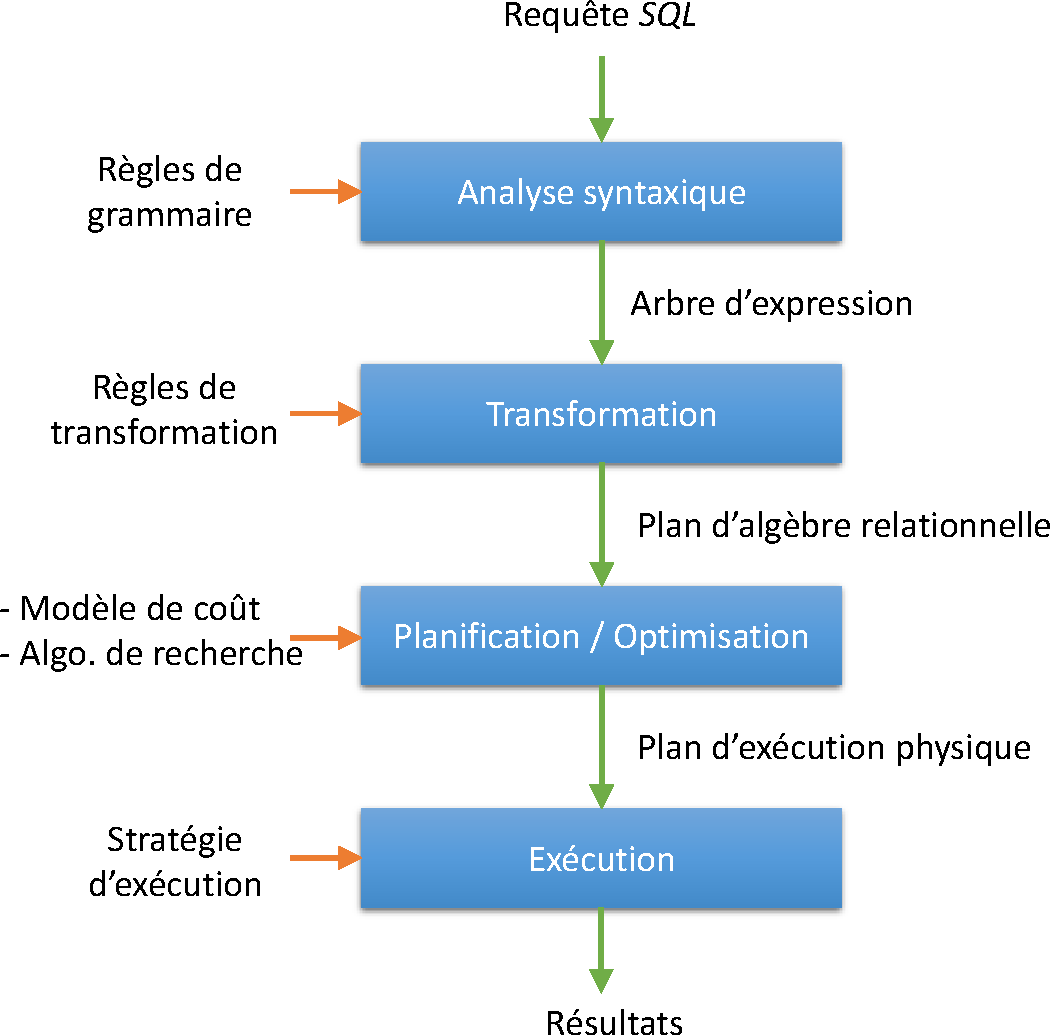
\includegraphics[scale=0.55]{chapitre2/chap2Fig/query-processing.pdf}
\caption{Architecture globale pour le traitement de requêtes dans un SGBD.}
 \label{fig:query-processing}
\end{center}
\end{figure}

\subsubsection{Analyse}
Le travail de l'analyseur est de prendre du texte écrit dans une langue comme SQL et de le convertir en un arbre d'analyse, qui est un arbre dont les nœuds correspondent soit à : (1) \textit{atomes}, qui sont des éléments lexicaux tels que des mots clés (par exemple, \texttt{SELECT}), des noms d'attributs ou de relations, des constantes, des parenthèses, des opérateurs tels que \texttt{+} ou \texttt{<}, et d'autres éléments de schéma, ou (2) des \textit{catégories syntaxiques}, qui sont des noms pour des sous-parties de requête qui ont un rôle similaire. Ils sont représentés par un nom descriptif entre les symboles \texttt{<} et \texttt{>} \cite{GarciaMolina08}. Par exemple, \texttt{<Requête>} est utilisé pour représenter une requête, et \texttt{<Condition>} représentera toute expression qui est une condition. Nous présenterons ces propos par un exemple dans la section suivante.

\paragraph{Une grammaire pour un sous-ensemble simple de SQL}
Nous allons illustrer le processus d'analyse en donnant quelques règles qui décrivent un petit sous-ensemble de requêtes SQL.

\subparagraph{Requête}
La catégorie syntaxique <Requête> est destinée à représenter certaines requêtes SQL. Nous lui donnons la règle :
\begin{verbatim}
<Requête> ::= SELECT <Sélection> FROM <Depuis> WHERE <Condition>
\end{verbatim}

Le symbole \microtypesetup{kerning=false}\texttt{::=}\microtypesetup{kerning=true} signifie << peut-être exprimer comme >>. Les catégories syntaxiques \texttt{<Sélection>}, \texttt{<Depuis>} et \texttt{<Condition>} représentent des listes pouvant suivre \texttt{SELECT}, \texttt{FROM} et \texttt{WHERE}, respectivement. Nous décrirons les formes de ces listes dans les prochaines sections.

\subparagraph{Sélection}
\begin{verbatim}
<Sélection> ::= <Attribut>, <Sélection>
<Sélection> ::= <Attribut>
\end{verbatim} 
Ces deux règles disent qu'une liste de sélection peut être une liste d'attributs séparés par des virgules : soit un attribut unique, soit un attribut, une virgule et toute liste d'un ou plusieurs attributs.

\subparagraph{Depuis}
\begin{verbatim}
<Depuis> ::= <Relation>, <Depuis>
<Depuis> ::= <Relation>
\end{verbatim}
Ici, une liste de type \texttt{Depuis} est définie comme étant une liste de relations séparées par des virgules.

\subparagraph{Condition}
Les règles que nous utiliserons sont :
\begin{verbatim}
<Condition> ::= <Condition> AND <Condition>
<Condition> ::= <Attribut> IN ( <Requête> )
<Condition> ::= <Attribut> = <Attribut>
<Condition> ::= <Attribut> LIKE <Motif>
\end{verbatim}

\subparagraph{Catégories syntaxiques}
Les catégories syntaxiques \texttt{<Attribut>}, \texttt{<Relation>} et \texttt{<Motif>} sont spéciales, puisqu'elles ne sont pas définies par des règles grammaticales, mais par des règles sur les atomes pour lesquels elles peuvent être utilisées. Par exemple, dans un arbre d'analyse, l'un des fils de \texttt{<Attribut>} peut être n'importe quelle chaîne de caractères qui identifie un attribut du schéma de base de données. De même, \texttt{<Relation>} peut être remplacé par n'importe quelle chaîne de caractères qui représente une relation dans le schéma, et \texttt{<Motif>} peut être remplacé par n'importe quelle chaîne entre guillemets qui est un modèle SQL légal.

\begin{example}\label{ex:parser-tree}
Notre étude de l'analyse et de la réécriture de requêtes sera basée sur notre exemple de gestion de vente. Nous voulons répondre à la requête << trouver les noms des clients qui ont payé leurs commandes en espèces >>. Nous identifions les clients qui ont payé des commandes en espèces en demandant si leur méthode de paiement est égale à << espèces >>, en utilisant l'opérateur \texttt{=}.
\end{example}

La requête SQL utilisé pour réponde à cette question est :
% \begin{verbatim}
% SELECT Nom
% FROM Clients, Commandes
% WHERE Clients.ClientsID = Commandes.ClientsID AND
%       Méthode_Paiement = 'espèces';
% \end{verbatim}
\begin{lstlisting}[language=Sql]
SELECT Nom
FROM Clients, Commandes
WHERE Clients.ClientsID = Commandes.ClientsID AND
      Méthode_Paiement = 'espèces';
\end{lstlisting}

L'arbre d'analyse pour notre requête, selon la grammaire que nous avons proposée, est illustré dans la \ref{fig:parser-tree}. A la racine se trouve la catégorie syntaxique \texttt{<Requête>}. En parcourant l'arbre, nous voyons que cette requête a une forme de \texttt{select-from-where}, la liste de \texttt{<Sélection>} se compose uniquement de l'attribut \texttt{Nom} et la liste de \texttt{<Depuis>} contient plus d'une relation et deux conditions connectées par \texttt{AND}.

\begin{figure}
\scriptsize
\begin{center}
\tikzset{>=latex}

\begin{forest} for tree={align=center}
[<Requête>
    [\texttt{SELECT}]
    [<Sélection>
        [<Attribut>
            [\texttt{Nom}]
        ]
    ]
    [\texttt{FROM}]
    [<Depuis>
		[<Relation>
			[\texttt{Clients}]
		]
		[\texttt{,}]
		[<Depuis>
			[<Relation>
				[\texttt{Commandes}]
			]
		]
    ]
    [\texttt{WHERE}]
    [<Condition>
		[<Condition>
			[<Attribut>
				[\texttt{ClientsID}]
			]
			[\texttt{=}]
			[<Attribut>
				[\texttt{ClientsID}]
			]
		]
		[\texttt{AND}]
		[<Condition>
			[<Attribut>
				[\texttt{Méthode\_Paiement}]
			]
			[\texttt{=}]
			[<Attribut>
				[\texttt{'espèces'}]
			]
		]
	]
]
\end{forest}
\caption{Exemple d'un arbre d'analyse.}
\label{fig:parser-tree}
\end{center}
\end{figure}

L'analyseur vérifie si une relation dans la requête est en réalité une vue virtuelle, chaque utilisation de cette relation dans la requête doit être remplacée par un arbre d'analyse qui décrit la vue \cite{GarciaMolina08}.
L'analyseur est aussi responsable de la vérification sémantique. Même si la requête est valable syntaxiquement, elle peut en fait violer une ou plusieurs règles sémantiques sur l'utilisation des noms. Par exemple, l'analyseur doit :

\begin{itemize}
 \item \textit{Vérifiez les relations} : Chaque relation mentionnée dans une clause \texttt{FROM} doit être une relation ou une vue dans le schéma de la base de données courante.
 \item \textit{Vérifiez et résoudre les attributs} : Chaque attribut mentionné dans la clause \texttt{SELECT} ou \texttt{WHERE} doit être un attribut d'une certaine relation dans la requête. Par exemple, l'attribut \texttt{Nom} est un attribut de \texttt{Clients}, donc l'analyseur valide cette utilisation. Il vérifie également l'ambiguïté, signalant une erreur si un attribut est dans la portée de deux ou plusieurs relations.
 \item \textit{Vérifiez les types} : Tous les attributs doivent être d'un type approprié à leurs utilisations. Par exemple, \texttt{Méthode\_Paiement} est utilisé dans une comparaison \texttt{=}, ce qui nécessite que cet attribut soit une chaîne ou un type qui peut être contraint à une chaîne. De même, les opérateurs sont vérifiés pour voir qu'ils s'appliquent aux valeurs des types appropriés et compatibles.
\end{itemize}

\subsubsection{Transformation}\label{sec:transformation}
Dans cette étape, l'arbre d'analyse résultant de l'étape précédente est transformé en une expression de l'algèbre relationnelle étendue.
L'objectif de la transformation des requêtes est : (1) la construction d'un arbre standardisé pour l'optimisation des requêtes (\textit{standardisation}), (2) l'élimination de la redondance (\textit{simplification}), et (3) la construction d'une expression améliorée (\textit{amélioration}) \cite{Jarke84}.
Nous verrons dans cette section comment appliquer des heuristiques qui améliorent l'expression algébrique de la requête, en utilisant certaines des nombreuses règles algébriques issues de l'algèbre relationnelle \cite{Elmasri08}. À titre préliminaire, cette section répertorie les règles algébriques qui transforment un arbre d'expression en un arbre d'expression équivalent qui peut avoir un plan de requête physique plus efficace. Le résultat de l'application de ces transformations algébriques est le plan de requête logique qui est la sortie de cette phase.

\paragraph{Règles algébriques pour améliorer les plans de requête}
Une règle est dite \textit{commutative} sur un opérateur si le résultat reste invariable si l'on intervertit les arguments de l'opérateur. Par exemple, $+$ et $\times$ sont des opérateurs commutatifs d'arithmétique. Plus précisément, $x + y = y + x$ et $x \times y = y \times x$ pour tout nombre $x$ et $y$. D'autre part, $-$ n'est pas un opérateur arithmétique commutatif : $x - y \neq y - x$.

Une règle est dite \textit{associative} sur un opérateur si nous pouvons regrouper deux utilisations de l'opérateur soit de la gauche ou de la droite. Par exemple, $+$ et $\times$ sont des opérateurs arithmétiques associatifs, ce qui signifie que $(x + y) + z = x + (y + z)$ et $(x \times y) \times z = x \times (y \times z)$. D'autre part, $-$ n'est pas associatif : $(x - y) - z \neq x - (y - z)$.

Nous allons présenter quelques règles de transformation de certain opérateurs SQL \cite{Freytag87, Elmasri08, GarciaMolina08}:

\begin{enumerate}
 \item \textbf{Décomposition de $\sigma$}. Une condition de sélection conjonctive peut être décomposée en une cascade (c'est-à-dire une séquence) d'opérations $\sigma$ individuelles :
 
 $\sigma_{c_1 \; \text{\texttt{AND}} \; c_2 \; \text{\texttt{AND}} \; \cdots \; \text{\texttt{AND}} \; c_n} (R) \equiv \sigma_{c_1} (\sigma_{c_2} (\cdots(\sigma_{c_n} (R))\cdots))$
 
 \item \textbf{Commutativité de $\sigma$}. L'opération de sélection $\sigma$ est commutative :
 
 $\sigma_{c_1} (\sigma_{c_2} (R)) \equiv \sigma_{c_2} (\sigma_{c_1} (R))$
 
 \item \textbf{Décomposition de $\pi$}. Dans une décomposition (séquence) d'opérations de projection $\pi$, tous sauf le dernier peuvent être ignorés :
 
 $\pi_{Liste_1}  (\pi_{Liste_2}  (\cdots(\pi_{Liste_n} (R))\cdots)) \equiv \pi_{Liste_1}(R)$
 
 \item \textbf{Commuter $\sigma$ avec $\pi$}. Si la condition de sélection $c$ ne concerne que les attributs $A_1, \cdots, A_n$ dans la liste de projection, les deux opérations peuvent être commutées :
 
 $\pi_{A_1, A_2, \cdots, A_n} (\sigma_c (R)) \equiv \sigma_c (\pi_{A_1, A_2, \cdots, A_n} (R))$
 
 \item \textbf{Commutativité de $\bowtie$ (et $\times$)}. L'opération de jointure est commutative, de même que l'opération de produit cartésien $\times$ :
 
 $R \bowtie_c S \equiv S \bowtie_c R$\\
 $R \times S \equiv S \times R$
 
 \item \textbf{Commuter $\sigma$ avec $\bowtie$ (ou $\times$)}. Si tous les attributs de la condition de sélection $c$ ne comportent que les attributs d'une des relations jointes, par exemple $R$, les deux opérations peuvent être commutées comme suit :
 
 $\sigma_c (R \bowtie S) \equiv (\sigma_c (R)) \bowtie S$
 
 \item \textbf{Commuter $\pi$ avec $\bowtie$ (ou $\times$)}. Supposons que la liste de projection est $L = {A_1, \cdots, A_n, B_1, \cdots, B_m}$, où $A_1, \cdots, A_n$ sont des attributs de $R$ et $B_1, \cdots, B_m$ sont des attributs de $S$. Si la condition de jointure $c$ implique seulement les attributs en $L$, les deux opérations peuvent être commutées comme suit :
 
 $\pi_L (R \bowtie_c S) \equiv (\pi_{A_1, \cdots, A_n} (R)) \bowtie_c (\pi_{B_1, \cdots ,B_m}(S))$
 
 \item \textbf{Commutativité des opérations ensemblistes}. Les opérations ensemblistes $\cup$ et $\cap$ sont commutatives, mais $-$ ne l'est pas.
 
 \item \textbf{Associativité de $\bowtie$, $\times$, $\cup$ et $\cap$}. Ces quatre opérations sont individuellement associatives; C'est-à-dire si les occurrences de $\theta$ représentent la même opération qui est l'une de ces quatre opérations, on a :
 
 $(R \; \theta \; S) \; \theta \; T \equiv R \; \theta \; (S \; \theta \; T)$
 
 \item \textbf{Commuter $\sigma$ avec des opérations ensemblistes}. L'opération $\sigma$ commute avec $\cup$, $\cap$ et $-$. Si $\theta$ représente l'une de ces trois opérations dans une expression, on a :
 
 $\sigma_c (R \; \theta \; S) \equiv (\sigma_c (R)) \; \theta \; (\sigma_c (S))$
 
 \item \textbf{L'opération $\pi$ commute avec $\cup$}.
 
 $\pi_L (R \cup S) \equiv (\pi_L (R)) \cup (\pi_L (S))$
 
 \item \textbf{Conversion d'une séquence ($\sigma$, $\times$) en $\bowtie$}. Si la condition $c$ d'une $\sigma$ qui suit un $\times$ correspond à une condition de jointure, convertissez la séquence ($\sigma$, $\times$) en une $\bowtie$ comme suit :
 
 $(\sigma_c (R \times S)) \equiv (R \bowtie_c S)$
 
 \item \textbf{Descendre $\sigma$ en bas en conjonction avec la différence ensembliste}.
 
 $\sigma_c (R - S) = \sigma_c (R) - \sigma_c ( S)$
 
 \item \textbf{Descendre $\sigma$ à un seul argument dans $\cap$}. Si dans la condition $\sigma_c$ tous les attributs sont de la relation $R$, alors :
 
 $\sigma_c (R \cap S) = \sigma_c (R) \cap \sigma_c (S)$
 
 \item \textbf{Élimination des doubles}. L'opérateur $\delta$ élimine les doublons d'un ensemble. Si $\theta$ représente l'une de ces trois opérations : $\bowtie$, $\bowtie_c$ ou $\times$, dans une expression, alors :
 
 $\delta(R \; \theta \; S ) \equiv \delta(R) \; \theta \; \delta(S)$\\
 $\delta(\sigma_c (R)) \equiv \sigma_c (\delta(R)).$
 
 \item \textbf{Règles de groupement et d’agrégation}. L'opérateur $\gamma$ a plusieurs règles, par exemple, il absorbe $\delta$. Nous pouvons projeter des attributs inutiles avant d'appliquer l'opération $\delta$. Nous pouvons également supprimer les doublons dans le cas d'agrégation de type \texttt{MIN} et \texttt{MAX} :
 
 $\delta (\gamma_L(R)) \equiv \gamma_L(R)$\\
 $\gamma_L (R) \equiv \gamma_L (\pi_M(R))$; Si $M$ est une liste contenant tous les attributs mentionnés dans $L$\\
 $\gamma_L (R) \equiv \gamma_L (\delta(R))$; $L$ est \texttt{MIN} et/ou \texttt{MAX}
 
 \item \textbf{Quelques transformations triviales}.\\
 Si $S$ est vide, alors $R \cup S = R$\\
 Si la condition $c$ dans $\sigma_c$ est vraie pour tout $R$, alors $\sigma_c (R) = R$
\end{enumerate}

\begin{example}\label{ex:transformation-query}
 Sur notre exemple de gestion de vente, supposons que nous voulons savoir pour chaque client la date de commande la plus récente. Nous pouvons exprimer cette requête comme :
\end{example}

% \begin{verbatim}
% SELECT Nom, MAX(Date_Com)
% FROM Clients, Commandes
% WHERE Clients.ClientsID = Commandes.ClientsID
% GROUP BY Nom;
% \end{verbatim}
\begin{lstlisting}[language=Sql]
SELECT Nom, MAX(Date_Com)
FROM Clients, Commandes
WHERE Clients.ClientsID = Commandes.ClientsID
GROUP BY Nom;
\end{lstlisting}

Un plan de requête logique initial construit directement à partir de la requête est représenté dans la \ref{fig:transformation1-tree}. La liste \texttt{FROM} est exprimée par un produit cartésien et la clause \texttt{WHERE} par une sélection. Le groupement et l'agrégation sont exprimés par l'opérateur $\gamma$. Nous pouvons appliquer les transformations suivantes :
\begin{enumerate}
 \item Combiner la sélection et le produit dans une jointure (règle 12).
 \item Générer un $\delta$ en dessous du $\gamma$ (règle 16).
 \item Générer un $\pi$ entre le $\gamma$ et le $\delta$ généré pour projeter sur \texttt{Nom} et \texttt{Date\_Com} (règle 16).
\end{enumerate}
Le plan résultant est représenté à la \ref{fig:transformation2-tree}. Nous pouvons maintenant pousser le $\delta$ sous la $\bowtie$ et introduire $\pi$ (règle 15). Ce nouveau plan de requête est représenté à la \ref{fig:transformation3-tree}. 

\begin{figure}
  \centering
  \small
  \subfloat[Plan de requête logique initial.\label{fig:transformation1-tree}]{
    %\resizebox{.28\textwidth}{!}
    {\tikzset{>=latex}

\begin{forest} for tree={align=center}
[$\gamma_{_{Nom, MAX(Date\_Com)}}$
    [$\sigma_{_{ClientsID = ClientsID}}$
		[$\times$
			[\texttt{Clients}]
			[\texttt{Commandes}]
		]
    ]
]
\end{forest}}
  }
  \quad
  \subfloat[Plan de requête après la première transformation.\label{fig:transformation2-tree}]{
    %\resizebox{.28\textwidth}{!}
    {\tikzset{>=latex}

\begin{forest} for tree={align=center}
[$\gamma_{_{Nom, MAX(Date\_Com)}}$
	[$\pi_{_{Nom, Date\_Com}}$
		[$\delta$
			[$\bowtie$\\$_{_{ClientsID = ClientsID}}$
				[\texttt{Clients}]
				[\texttt{Commandes}]
			]
		]
    ]
]
\end{forest}
}
  }
  \quad
  \subfloat[Plan de requête après la deuxième transformation.\label{fig:transformation3-tree}]{
    %\resizebox{.34\textwidth}{!}
    {\tikzset{>=latex}

\begin{forest} for tree={align=center}
[$\gamma_{_{Nom, MAX(Date\_Com)}}$
	[$\pi_{_{Nom, Date\_Com}}$
		[$\bowtie$\\$_{_{ClientsID = ClientsID}}$
			[$\delta$
				[$\pi_{_{Nom, ClientsID}}$
					[\texttt{Clients}]
				]
			]
			[$\delta$
				[$\pi_{_{Date\_Com, ClientsID}}$
					[\texttt{Commandes}]
				]
			]
		]
    ]
]
\end{forest}
}
  }
  \caption{Étape de transformation du plan de requête logique pour l'\ref{ex:transformation-query}.}\label{fig:transformation-tree}
\end{figure}

\paragraph{Amélioration du plan de requête logique}
Il existe un certain nombre de règles algébriques qui améliorent les plans de requêtes logiques. Les règles suivantes sont les plus couramment utilisées par les optimiseurs \cite{GarciaMolina08, Elmasri08}:
\begin{itemize}
 \item Les sélections peuvent être poussées vers le bas dans l'arborescence d'expression dans la mesure du possible. Si une condition de sélection est composée de \texttt{AND} de plusieurs conditions, nous pouvons diviser la condition et pousser chaque partie vers le bas de l'arbre séparément. Cette stratégie est probablement la technique d'amélioration la plus efficace.
 \item De même, les projections peuvent être poussées vers le bas de l'arbre, ou de nouvelles projections peuvent être ajoutées.
 \item Les opérations d'éliminations des doubles peuvent parfois être supprimées ou déplacées vers une position plus pratique dans l'arborescence.
 \item Certaines sélections peuvent être combinées avec un produit ci-dessous pour transformer la paire d'opérations en une jointure, ce qui est généralement beaucoup plus efficace à évaluer que les deux opérations séparément.
\end{itemize}

\begin{example}\label{ex:transformation-query2}
 Considérons l'arbre d'analyse de la \ref{fig:parser-tree}. L'expression d'algèbre relationnelle résultante après la transformation de cet arbre est illustrée dans la \ref{fig:transformation1-tree2}. Maintenant, nous voulons appliquer les nouvelles règles de transformation. Tout d'abord, nous pouvons diviser les deux parties de la sélection en \texttt{ClientsID = ClientsID} et \texttt{Méthode\_Paiement = 'espèces'}. Ce dernier peut être poussé vers le bas de l'arbre, puisque le seul attribut impliqué, \texttt{Méthode\_Paiement}, est de la relation \texttt{Commandes}. Ensuite, la sélection et le produit peuvent être combiné dans une seule jointure. L'effet de ces transformations est démontré sur la \ref{fig:transformation2-tree2}.
\end{example}

\begin{figure}
  \centering
  \footnotesize
  \subfloat[Plan de requête logique initial.\label{fig:transformation1-tree2}]{
    %\resizebox{.28\textwidth}{!}
    {\tikzset{>=latex}

\begin{forest} for tree={align=center}
[$\pi_{_{Nom}}$
	[$\sigma_{{ClientsID = ClientsID \; AND \; Méthode\_Paiement = 'espèces'}}$
		[$\times$
			[\texttt{Clients}]
			[\texttt{Commandes}]
		]
	]
]
\end{forest}
}
  }
  \quad
  \subfloat[Plan de requête après la transformation.\label{fig:transformation2-tree2}]{
    %\resizebox{.28\textwidth}{!}
    {\tikzset{>=latex}

\begin{forest} for tree={align=center}
[$\pi_{_{Nom}}$
	[$\bowtie$\\$_{{ClientsID = ClientsID}}$
		[\texttt{Clients}]
		[$\sigma_{{Méthode\_Paiement = 'espèces'}}$
			[\texttt{Commandes}]
		]
	]
]
\end{forest}
}
  }
  \caption{Transformation du plan de requête logique pour l'\ref{ex:parser-tree}.}\label{fig:transformation-tree2}
\end{figure}

\subsubsection{Génération des plans et optimisation}\label{sec:planningOptimisation}
Après avoir analysé et transformé une requête en un plan de requête logique, la prochaine étape consiste à transformer le plan logique en un plan physique. Cela se fait normalement en considérant plusieurs plans physiques qui sont dérivés du plan logique, et en évaluant ou en estimant le coût de chacun. Après cette évaluation, souvent appelée génération de plans basée sur le \textit{modèle coût} \cite{Selinger79}, le plan de requête physique avec le coût le moins estimé est choisi. Ce plan est passé au moteur d'exécution de requêtes \cite{GarciaMolina08}. La \ref{fig:query-optimization} donne un aperçu du processus d'optimisation des requêtes.

Le premier problème est de savoir comment estimer les coûts des plans avec précision. Ces estimations sont basées sur (1) des statistiques sur données de la base, et (2) des statistiques de système. Compte tenu des valeurs de ces paramètres, nous pouvons faire un certain nombre d'estimations raisonnables de la taille des relations qui peuvent être utilisés pour prédire le coût d'un plan physique complet.

\paragraph{Statistiques sur les données}
Étant donné un arbre d'opérateur d'une requête, il est d'une importance fondamentale d'être en mesure d'évaluer avec \textit{précision} et \textit{efficacité} son coût. L'estimation des coûts doit être précise parce que l'optimisation est seulement aussi bonne que ses estimations de coûts. L'estimation des coûts doit être efficace car elle est dans la boucle interne de l'optimisation des requêtes et est invoquée à plusieurs reprises \cite{Chaudhuri98}.
Un SGBD moderne permet généralement à l'utilisateur ou à l'administrateur de demander explicitement la collecte de statistiques telles que $T(R)$, le nombre de tuples dans une relation $R$, et $V(R, a)$, le nombre de valeurs différentes dans la colonne de relation $R$ pour l'attribut $a$. Ces statistiques sont ensuite utilisées dans l'optimisation des requêtes, inchangées jusqu'à la prochaine commande de collecte de statistiques \cite{GarciaMolina08}. Généralement, les statistiques sont sauvegardées dans la base de données comme relations appelées \textit{catalogue} ou \textit{dictionnaire de données} \cite{Elmasri08}.

\begin{figure}
\begin{center}
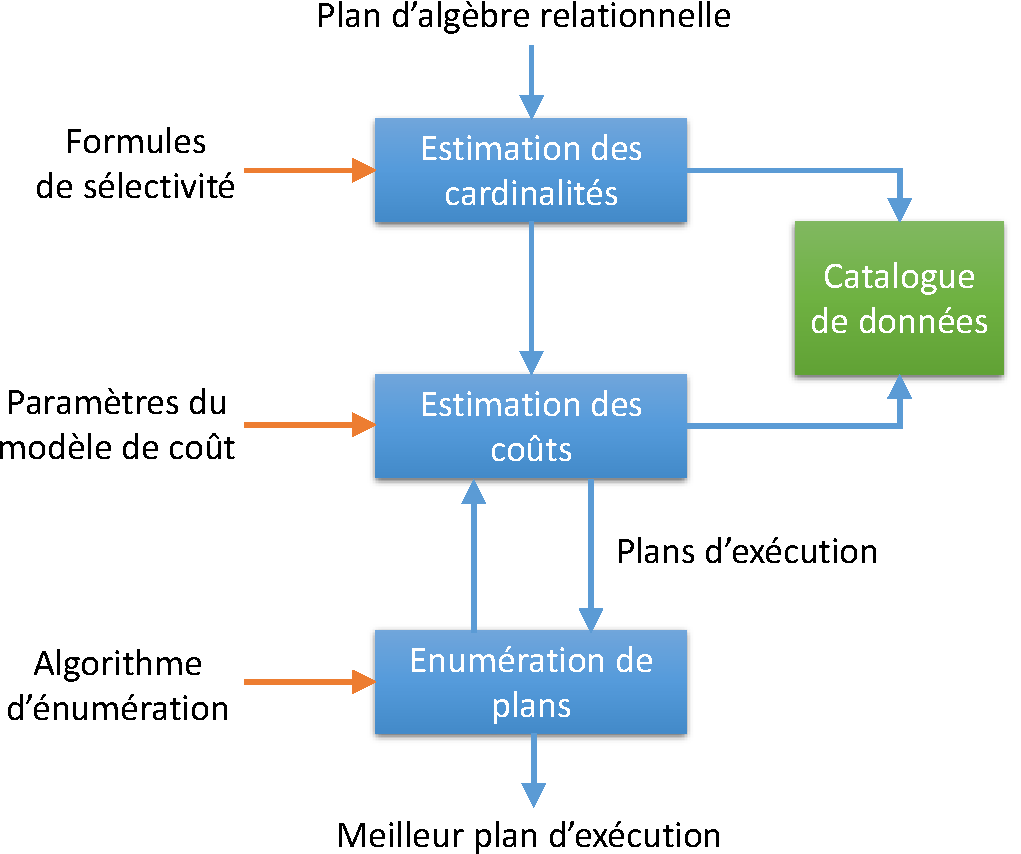
\includegraphics[scale=0.55]{chapitre2/chap2Fig/query-optimization.pdf}
\caption{Une architecture globale pour l'étape d'optimisation de requêtes.}
 \label{fig:query-optimization}
\end{center}
\end{figure}

En balayant entièrement la relation $R$, il est facile de compter le nombre de tuples $T(R)$ et aussi de découvrir le nombre de valeurs $V(R, a)$ différentes pour chaque attribut $a$. De plus, un SGBD peut calculer un \textit{histogramme} de distribution des valeurs d'un attribut donné. Si $V(R, A)$ n'est pas trop grand, l'histogramme peut être constitué du nombre (ou fraction) des tuples ayant chacune des valeurs de l'attribut $a$. Les histogrammes les plus courants sont \cite{Poosala96} :
\begin{itemize}
 \item \textbf{Largeur égale.} Divise l'intervalle de valeurs en intervalles de taille égale. On choisit une largeur $w$, avec une constante $v_0$. On fournit des comptages du nombre de tuples avec des valeurs $v$ dans les intervalles $v_0 \leq v < v_0 + w$, $v_0 + w \leq v < v_0 + 2 w$, etc. La valeur $v_0$ peut être la valeur la plus petite ou une borne inférieure sur les valeurs vues jusqu'ici.
 \item \textbf{Hauteur égale.} Ajuste les limites des intervalles de sorte que chaque intervalle ait le même nombre de valeurs. Ce sont les << centile\footnote{Un centile est chacune des 99 valeurs qui divisent les données triées en 100 parts égales, de sorte que chaque partie représente 1/100 de l'échantillon de population.} >> courants. On choisit une fraction $p$, et on énumère la valeur la plus petite, la valeur qui est la fraction $p$ du plus bas, la fraction $2p$ du plus bas, et ainsi de suite, jusqu'à la valeur la plus grande.
 \item \textbf{Valeurs les plus fréquentes.} Nous pouvons énumérer les valeurs les plus communes et leur nombre d'occurrences.
\end{itemize}

Les SGBD modernes comme IBM DB2, Informix, Microsoft SQL Server, Oracle et Sybase ASE utilisent la technique d'histogramme pour générer les statistiques sur les données \cite{Ramakrishnan03}.

\begin{figure}
  \centering
  \subfloat[Histogramme hauteur égale.\label{fig:histo-equidepth}]{
    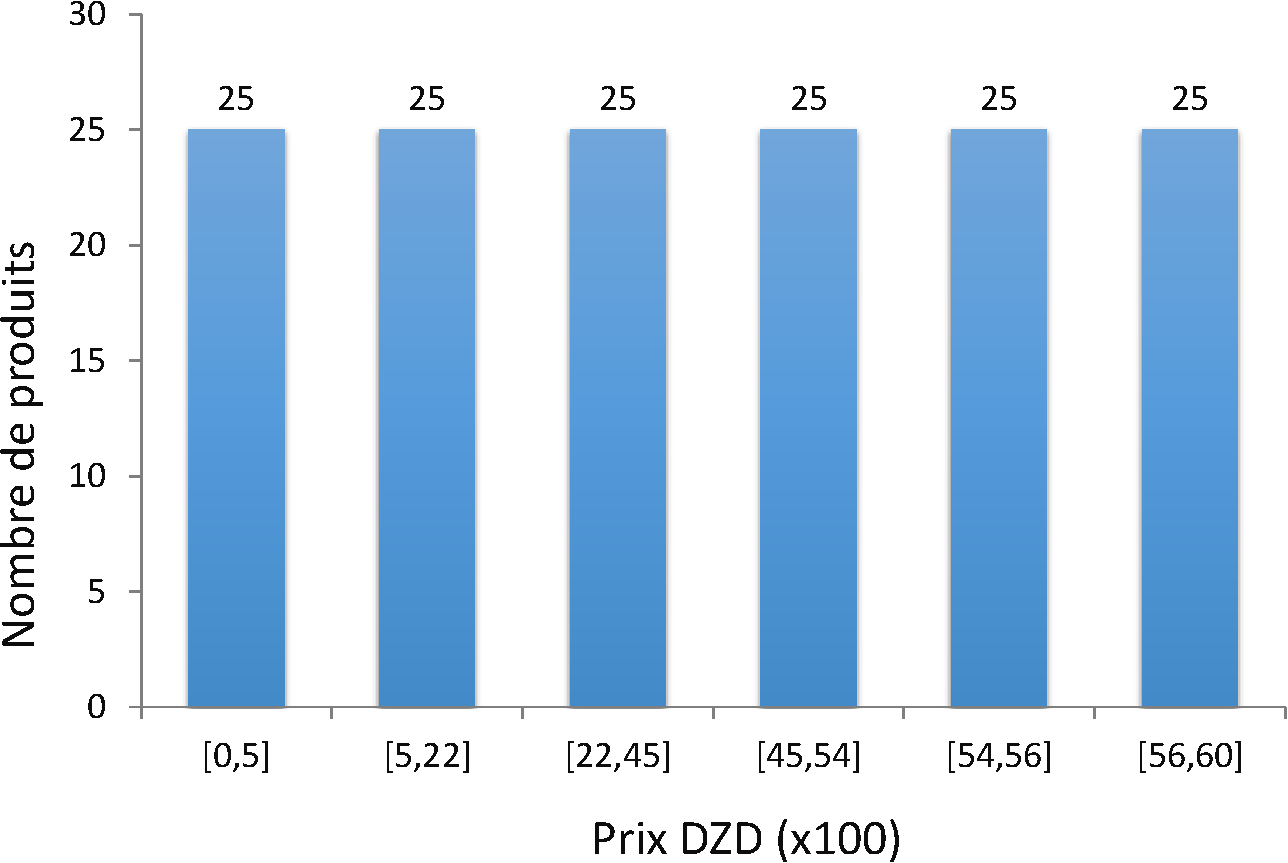
\includegraphics[scale=0.33]{chapitre2/chap2Fig/histo-equidepth.pdf}
  }
  \quad
  \subfloat[Histogramme largeur égale.\label{fig:histo-equiwidth}]{
    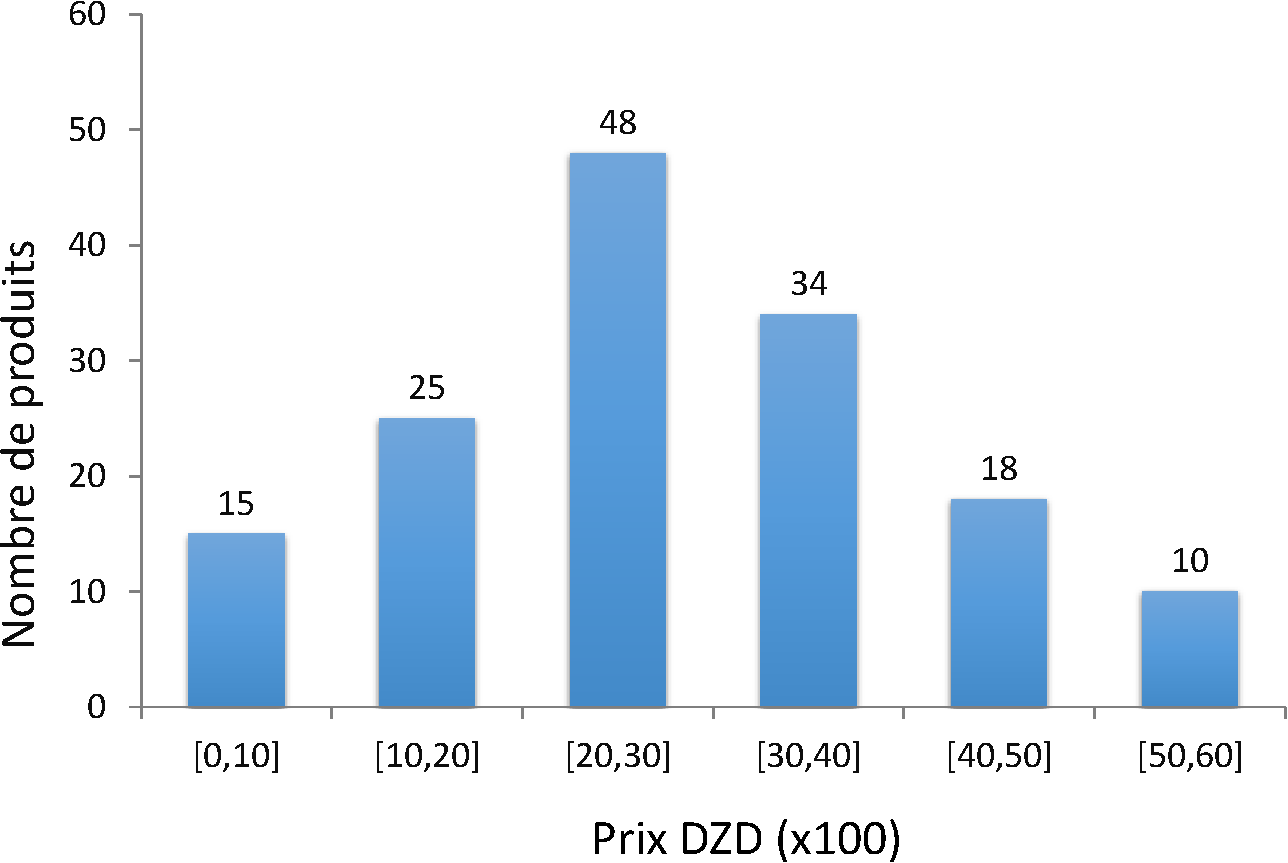
\includegraphics[scale=0.33]{chapitre2/chap2Fig/histo-equiwidth.pdf}
  }
  \caption{Exemples des histogrammes de distribution des valeurs d'attribut \textit{Prix} de la table \textit{Produit}.}\label{fig:histo-types}
\end{figure}

%\paragraph{Estimation de la taille des résultats intermédiaires}

\paragraph{Statistiques de système}\label{sec:costModelPram}
Le coût de l'évaluation des requêtes peut être mesuré en fonction d'un certain nombre de ressources système différentes. Les ressources ou paramètres les plus importants sont les suivants :

\begin{itemize}
 \item \textbf{Coût d'accès au stockage secondaire.} C'est le coût du transfert (lecture et écriture) des blocs de données entre le stockage de disque secondaire et les tampons de mémoire principale. Cela est également connu sous le nom de coût d'E/S (entrée/sortie) ou $\mathcal{C_{E/S}}$. Le coût de la recherche d'enregistrements dans un fichier disque dépend du type de structures d'accès sur ce fichier et la nature d'allocation des blocs de fichiers.
 \item \textbf{Coût de stockage sur disque.} C'est le coût de stockage sur disque de tous les fichiers intermédiaires générés par une stratégie d'exécution de la requête.
 \item \textbf{Coût de calcul.} C'est le coût d'exécution des opérations sur les enregistrements en mémoire tampon pendant l'exécution de la requête. Ces opérations comprennent la recherche, le tri, la fusion d'enregistrements pour une opération de jointure ou de tri et l'exécution de calculs sur les valeurs. Cela est également connu comme le coût de CPU (unité centrale de traitement) ou $\mathcal{C_{CPU}}$.
 \item \textbf{Coût d'utilisation de la mémoire.} C'est le coût correspondant au nombre de tampons mémoire nécessaires pendant l'exécution de la requête.
 \item \textbf{Coût de la communication.} Il s'agit du coût d'expédition de la requête et de ses résultats à partir du site de base de données vers le site ou le terminal d'où provient la requête. Dans les bases de données distribuées, il inclut également le coût du transfert des tables et des résultats entre différents ordinateurs au cours de l'évaluation des requêtes. Le coût de communication est abrégé $\mathcal{C_{COM}}$.
\end{itemize}

\subparagraph{Obtention des paramètres et leurs relations}
Les paramètres du modèle de coût, tels que le coût d'E/S et de CPU, doivent être calculés. Trois méthodes existent dans la littérature pour obtenir ces paramètres : \textit{analytique}, \textit{empirique} et \textit{dynamique} \cite{Ozsu11}.

\begin{enumerate}
 \item \textbf{Méthode analytique.} C'est l'approche classique employée par les premiers travaux sur les modèles de coût. Elle utilise des connaissances \textit{détaillées} sur le SGBD, l'implémentation des opérateurs algébriques, ainsi que les caractéristiques externes du matériel, pour déterminer analytiquement les informations sur les coûts \cite{Selinger79,Graefe93,Haas97}. Cette approche est adaptée par le SGBD open-source PostgreSQL \cite{Wu13b}.
 \item \textbf{Méthode empirique.} Cette approche traite le SGBD comme une \textit{boîte noire}. Elle consiste à identifier d'abord un ensemble de caractéristiques de requête et de données qui déterminent potentiellement les coûts des opérateurs. Puis, exécuter ces requêtes d'apprentissages sur le système. Ensuite, appliquer des modèles \textit{statistiques} ou \textit{d'apprentissage automatique} aux données collectées, et à partir de ceux-ci déterminer les paramètres finaux du modèle de coût et la relation entre eux \cite{Wu13,Ganapathi09,Li12a}. Cette approche est également utilisée par les SGBD commerciaux comme Oracle \cite{Chakkappen08}.
 \item \textbf{Méthode dynamique.} Les méthodes précédentes supposent que l'environnement d'exécution est toujours stable. Cependant, dans la plupart des cas, les facteurs d'environnement d'exécution changent fréquemment, tels que la charge et la vitesse du CPU, le débit d'E/S, la disponibilité de mémoire, le schéma et les données de la BD, etc. Cette troisième approche se base sur la méthode empirique, et de plus, elle surveille le comportement d'exécution du SGBD et collecte et ajuste dynamiquement les informations sur les coûts pour faire face au changement d'environnement \cite{Duan09,Sheikh11,Khattab13}.
\end{enumerate}

% TODO: 
% Weighted sum of costs
% C_Q = $\mathcal{C_{e/s}$ + $\mathcal{C_{cpu}$ + $\mathcal{C_{com}$

%\paragraph{Modèles de coût des opérateurs}
Compte tenu d'un plan d'exécution, nous pouvons maintenant estimer son coût en utilisant l'estimation de la cardinalité des résultats intermédiaires faite par les techniques de \ref{sec:cardinalityEstimation} de l'\ref{annex:CostModelEstimations}, couplées aux estimations de coûts pour divers algorithmes et méthodes d'accès décrits au \ref{sec:operatorsCostModel} de l'\ref{annex:CostModelEstimations}.

\paragraph{Approches pour l'énumération des plans physiques} % 16.5.4 Approaches to Enum erating Physical Plans (db complete book)
Maintenant, considérons l'utilisation des estimations de coûts dans la conversion d'un plan de requête logique en un plan de requête physique. L'approche de référence, appelée \textit{exhaustive}, consiste à considérer toutes les combinaisons de choix possible. Chaque plan physique est affecté à un coût estimé, et celui avec le plus petit coût est sélectionné \cite{Elmasri08}. Cependant, il existe d'autres approches pour sélectionner un plan physique. En terme d'exploration de l'espace des plans physiques possibles, il existe deux approches principales : (1) \textit{descendante} et (2) \textit{ascendante}. Dans la première approche, l'estimation se fait à partir de la racine de l'arbre du plan de requête logique vers le bas en choisissant le meilleur choix à chaque étape. Cette approche est adoptée par Volcano, Cascades, Tandem et Microsoft SQL Server \cite{Lohman07}. Tandis que dans la deuxième approche, l'estimation se fait à partir des feuilles vers la racine. Cette approche est utilisée dans System R, DB2, Oracle et Informix \cite{Lohman07}. Nous décrirons ensuite les différentes techniques proposées dans la littérature pour l'énumération des plans physiques \cite{GarciaMolina08, Elmasri08}.

\begin{itemize}
 \item \textbf{Sélection heuristique.} Une option est d'utiliser la même approche pour sélectionner un plan physique qui est généralement utilisé pour sélectionner un plan logique : faire une séquence de choix basée sur l'heuristique (\ref{sec:transformation}). Il existe d'autres heuristiques qui peuvent être appliquées. Par exemple, si le plan logique appelle une sélection $\sigma_{A=c}(R)$, et la relation stockée $R$ a un index sur l'attribut $A$, effectuer un balayage d'index pour obtenir seulement les tuples de $R$ avec une valeur de $A$ égale à $c$.
 \item \textbf{Séparation et évaluation (\textit{Branch-and-Bound}).} Cette approche, souvent utilisée en pratique, commence par utiliser des heuristiques pour trouver un bon plan physique pour l'ensemble du plan de requête logique. Soit $\mathcal{C}$ le coût de ce plan. Alors, lorsque nous considérons d'autres plans pour les sous-requêtes, nous pouvons éliminer tout plan qui a un coût supérieur à $\mathcal{C}$, puisque ce plan ne pourrait pas participer à un plan complet meilleur que celui que nous avons déjà. De même, si nous trouvons un plan qui a un coût moins que $\mathcal{C}$, nous remplaçons $\mathcal{C}$ par le coût de ce meilleur plan dans l'exploration ultérieure de l'espace des plans de requêtes physiques.
 \item \textbf{Escalade (\textit{Hill climbing}).} Cette approche, dans laquelle nous cherchons une << vallée >> dans l'espace des plans physiques et de leurs coûts, commence avec un plan physique heuristiquement choisi. Nous pouvons alors apporter de petits changements au plan, par exemple en remplaçant une méthode pour exécuter un opérateur par une autre, ou en réordonnant des jointures en utilisant les lois associatives et/ou commutatives, pour trouver des plans << proches >> qui ont un coût inférieur. Lorsque nous trouvons un plan tel qu'aucune modification ne permet pas de donner un plan de coût inférieur, nous choisissons ce plan comme un plan physique.
 \item \textbf{Programmation dynamique.} Dans cette variante de la stratégie ascendante, nous gardons pour chaque sous-expression seulement le plan de moindre coût. Au fur et à mesure que nous traversons l'arbre, nous considérons les implémentations possibles de chaque nœud, en supposant que le meilleur plan pour chaque sous-expression est également utilisé.
 \item \textbf{System-R.} Cette approche améliore l'approche de programmation dynamique en gardant pour chaque sous-expression non seulement le plan de moindre coût, mais certains autres plans qui ont un coût plus élevé, alors qu'ils produisent un résultat trié dans un ordre qui peut être utile plus haut dans l'expression de l'arbre. Car les attributs déjà triés dans une opération tel que la sélection, le groupement ou la jointure peuvent être utilisés dans un algorithme de tri d'une manière efficace \cite{Selinger79}.
\end{itemize}

\begin{figure}
  \centering
  %\small
  \subfloat[Arbre de jointure linéaire gauche.\label{fig:left-deep-join-tree}]{
    {\tikzset{>=latex}

\begin{forest} for tree={align=center}
[$\bowtie$
    [$\bowtie$
		[$\bowtie$
			[$R$]
			[$S$]
		]
		[$T$]
    ]
    [$U$]
]
\end{forest}
}
  }
  \quad
  \subfloat[Arbre de jointure ramifié.\label{fig:bushy-join-tree}]{
    {\begin{forest} for tree={align=center}
[$\bowtie$
	[$\bowtie$
		[$R$]
		[$S$]
	]
    [$\bowtie$
		[$T$]
		[$U$]
    ]
]
\end{forest}
}
  }
  \quad
  \subfloat[Arbre de jointure linéaire droit.\label{fig:right-deep-join-tree}]{
    {\begin{forest} for tree={align=center}
[$\bowtie$
	[$R$]
    [$\bowtie$
		[$S$]
		[$\bowtie$
			[$T$]
			[$U$]
		]
    ]
]
\end{forest}
}
  }
  \caption{Exemple des méthodes pour la jointure de quatre relations.}\label{fig:join-tree-examples}
\end{figure}

\subparagraph{Problème d'ordre de jointure} % 19.5.3 Multirelation Queries and JOIN Ordering Choices
Les règles de transformation algébriques pour l'opération de jointure peuvent produire de nombreuses expressions de jointure équivalentes. En conséquence, le nombre d'arborescences de requêtes alternatives croît très rapidement avec l'augmentation du nombre de jointures dans une requête. En général, pour un bloc de requête comportant $n$ relations, il existe $n!$ ordres de jointure \cite{Elmasri08}.
Un arbre d'une requête ayant plus de deux jointures peut être exprimé en trois structures : 
\begin{enumerate}
 \item \textbf{Arbre de jointure linéaire gauche.} Est un arbre binaire où l'enfant gauche de chaque nœud de feuille est une relation de base (\ref{fig:left-deep-join-tree}).
 \item \textbf{Arbre de jointure linéaire droit.} Est un arbre binaire dans lequel l'enfant droit de chaque nœud non-feuille est toujours une relation de base. Un exemple est illustré dans la \ref{fig:right-deep-join-tree}.
 \item \textbf{Arbre de jointure ramifié.} Est un arbre binaire où l'enfant gauche ou droit d'un nœud interne peut être un nœud de jointure (\ref{fig:bushy-join-tree}). 
\end{enumerate}

La plupart des optimiseurs de requêtes considèrent les arbres de jointure linéaire gauche comme arbre de jointure préféré, puis choisi un parmi les $n!$ ordres de jointure possibles. Le problème d'ordre de jointure peut être résolu par trois classes d'algorithme : déterministe, aléatoire ou génétique (pour plus de détails, voir l'étude de \cite{Vellev09}).

\begin{itemize}
 \item \textbf{Algorithmes déterministes.} Également connu sous le nom d'algorithme de programmation dynamique de recherche exhaustive. Les algorithmes de cette classe effectuent une certaine recherche déterministe de l'espace de solution, soit par traverse complète, soit par l'application de certaines heuristiques d'élagage de l'espace \cite{Selinger79,Steinbrunn97}.
 \item \textbf{Algorithmes aléatoires.} Ces algorithmes effectuent une marche aléatoire dans l'espace de la solution, se déplaçant d'un point à un autre. Un déplacement est possible si la solution du premier point peut être transformée en solution du second point en lui appliquant une seule règle de transformation. L'exécution de l'algorithme se termine soit quand aucun déplacement valide ne peut être effectué ou quand un temps d'exécution prédéfini s'est écoulé. La meilleure solution trouvée pendant la marche aléatoire est le résultat de l'optimisation \cite{Ioannidis87,Ioannidis90}.
 \item \textbf{Algorithmes génétiques.} Les algorithmes génétiques imitent l'évolution biologique pour rechercher la solution optimale. L'idée principale est, à partir d'un ensemble initial (population) de solutions, génère des descendants par des opérations de croisement aléatoire et mutation. Les meilleurs individus de la population survivent à chaque génération et forment la nouvelle population. L'algorithme s'arrête soit après un certain nombre de générations, soit lorsque la population devient homogène au-dessus d'un certain seuil suivant de la fonction de coût \cite{Bennett91,Stillger96}.
\end{itemize}

\subsubsection{Exécution}
La dernière étape du processus est l'exécution de la requête. Dans cette étape, toutes les opérations d'E/S et de CPU indiquées dans le plan physique sont exécutées.
Un opérateur physique d'une requête peut être exécuté en mode \textit{matérialisé} ou \textit{pipeline} et/ou \textit{parallèle}.

\paragraph{Matérialisée}
Avec une exécution matérialisée, le résultat d'une opération est stocké comme une relation temporaire. Chaque résultat est physiquement matérialisé sur le dispositif de stockage et s'ajoute au coût global du traitement des requêtes. Par exemple, le résultat de l'opération $\bowtie$ peut être calculée et stocké comme une relation temporaire. Ce résultat est considéré comme entrée par l'algorithme qui calcule l'opération $\pi$ pour produire le résultat final de la requête. La génération et le stockage de gros fichiers temporaires sur le disque prend beaucoup de temps et peuvent être inutile dans de nombreux cas, car ces fichiers seront immédiatement utilisés comme entrée pour la prochaine opération \cite{Elmasri08}.

\paragraph{Pipeline}
D'autre part, avec l'exécution en pipeline, lorsque les tuples résultants d'une opération sont produits, ils sont envoyés directement à l'opération suivante dans la séquence de requête. Par exemple, les tuples sélectionnés d'une relation sont produits par l'opération $\sigma$, et placés dans un tampon mémoire. L'opération $\bowtie$ consomme alors les tuples de la mémoire tampon, et les tuples qui résultent sont pipelinés à l'opération $\pi$. L'avantage du pipelining est les économies de coût d'écriture des résultats intermédiaires sur le disque et la relecture pour l'opération suivante. Il permet également de produire des résultats rapidement avec certaines opérations algébriques.

\begin{figure}
\begin{center}
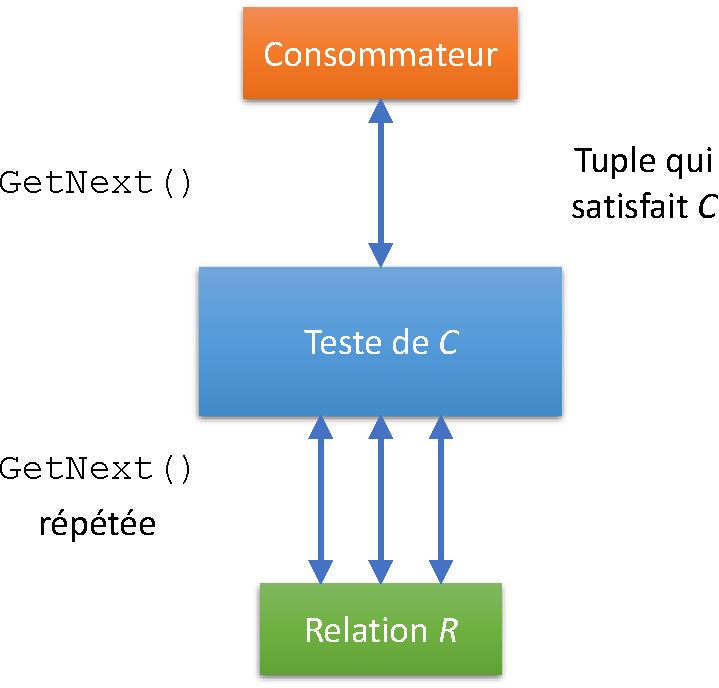
\includegraphics[scale=0.55]{chapitre2/chap2Fig/pipeline-example.pdf}
\caption{Exécution d'une sélection en mode pipeline à l'aide d'itérateurs.}
 \label{fig:pipeline-example}
\end{center}
\end{figure}

Différents algorithmes pour des opérations algébriques impliquent la lecture d'un ou plusieurs fichiers comme entrée, le traité, et ensuite la génération d'un fichier de résultat comme sortie. Si l'opération est mise en œuvre de telle sorte qu'elle produit qu'un tuple à la fois, elle peut être considérée comme un \textit{itérateur}. Par exemple, une implémentation pour la jointure à boucle imbriquée génère un tuple à la fois comme sortie après chaque jointure. L'interface itérateur comprend généralement les méthodes suivantes \cite{chaudhuri04} :

\begin{enumerate}
 \item \textbf{\texttt{Open()}} : Cette méthode initialise l'opérateur en allouant des tampons pour son entrée et sa sortie et en initialisant toutes les structures de données nécessaires à l'opérateur. Il est également utilisé pour transmettre des arguments tels que les conditions de sélection nécessaires pour effectuer l'opération. Il appelle à son tour \texttt{Open()} pour obtenir les arguments dont il a besoin.
 \item \textbf{\texttt{GetNext()}} : Cette méthode appelle le \texttt{GetNext()} sur chacun de ses arguments d'entrée et appelle le code spécifique à l'opération exécutée sur les entrées. Le prochain tuple de sortie généré est renvoyé, et l'état de l'itérateur est mis à jour suivant la quantité d'entrée traitée. Lorsque aucun tuple ne peut être renvoyé, il place une valeur spéciale dans le tampon de sortie.
 \item \textbf{\texttt{Close()}} : Cette méthode met fin à l'itération après la génération de tous les tuples possible ou si le nombre requis/demandé de tuples a été retourné. Elle appelle également \texttt{Close()} sur les arguments de l'itérateur.
\end{enumerate}

Cependant, certains opérateurs physiques ne supportent pas le concept d'interface itérateur et ne peuvent donc pas prendre en charge le pipeline. Comme par exemple l'opérateur de tri et de groupement, car ils ne produisent aucune sortie tant qu'ils n'ont pas consommé leurs entrées complètement \cite{luo04}.

\begin{example}
 Le consommateur du résultat du pipeline appelle \texttt{GetNext()} chaque fois qu'un tuple est nécessaire. Dans le cas d'une projection, il suffit d'appeler \texttt{GetNext()} une fois sur la source des tuples, ensuite projeter ce tuple de manière appropriée et retourner le résultat au consommateur. Pour une sélection $\sigma_c$, il peut être nécessaire d'appeler \texttt{GetNext()} plusieurs fois à la source, jusqu'à ce qu'un tuple qui satisfait la condition $C$ est trouvé. La \ref{fig:pipeline-example} illustre ce processus.
\end{example}

\paragraph{Parallèle}
Les opérations de base de données, qui prennent souvent beaucoup de temps et impliquent beaucoup de données, peuvent généralement bénéficier d'un traitement parallèle. Trois approches principales ont été proposées pour les bases de données parallèles. Ils correspondent à trois configurations matérielles différentes de processeurs et de périphériques de stockage secondaires (disques) pour supporter le parallélisme. Dans une \textit{architecture à mémoire partagée}, plusieurs processeurs sont connectés à un réseau d'interconnexion et peuvent accéder à une région de mémoire principale commune. Le deuxième type d'architecture est connu sous le nom \textit{d'architecture à disque partagé}. Dans cette architecture, chaque processeur a sa propre mémoire, qui n'est pas accessible à partir d'autres processeurs. Cependant, chaque machine a accès à tous les disques à travers le réseau d'interconnexion. Le troisième type est \textit{l'architecture sans partage}. Dans cette architecture, chaque processeur accède à sa propre mémoire principale et à son stockage disque \cite{Taniar08}.

L'architecture sans partage offre la possibilité d'atteindre le parallélisme dans le traitement des requêtes à quatre niveaux, y compris (1) le parallélisme inter-requêtes, (2) le parallélisme intra-requêtes, (3) le parallélisme inter-opérations et (4) le parallélisme intra-opérations \cite{Ozsu11}.

\begin{enumerate}
 \item \textbf{Parallélisme inter-requêtes.} Le parallélisme inter-requêtes est le << parallélisme entre les requêtes >>, c'est-à-dire que des requêtes ou des transactions différentes sont exécutées en parallèle les unes avec les autres d'une façon concurrente. L'utilisation principale du parallélisme entre les requêtes consiste à mettre à l'échelle les systèmes de traitement des transactions pour supporter un grand nombre de transactions par seconde.
 \item \textbf{Parallélisme intra-requêtes.} Une requête est divisée en plusieurs opérations. Le parallélisme intra-requête est une exécution d'une seule requête en parallèle sur plusieurs processeurs et disques. Dans ce cas, les opérations multiples dans une requête sont exécutées en parallèle. Par conséquent, le parallélisme intra-requête est le << parallélisme au sein d'une requête >>.
 \item \textbf{Parallélisme inter-opérations.} Puisque les opérations de base de données fonctionnent sur des tables contenant de grands ensembles de données, nous pouvons paralléliser les opérations en les exécutant en parallèle sur différents sous-ensembles de la table. Par conséquent, le parallélisme inter-opérations est souvent appelé parallélisme partitionné, c'est-à-dire parallélisme dû à la partition des données. Comme le nombre d'enregistrements dans une table peut être important, le degré de parallélisme est potentiellement énorme. Par conséquent, le parallélisme inter-opérations est naturel dans les systèmes de base de données.
 \item \textbf{Parallélisme intra-opérations.} Le parallélisme intra-opérations est là où le parallélisme est créé en exécutant simultanément différentes opérations au sein d'une même requête. Par exemple, la séquence d'opérations $R \bowtie S \bowtie T \bowtie U$. Dans ce cas, on peut traiter le $R \bowtie S$ en parallèle avec le $T \bowtie U$.
\end{enumerate}

% TODO: Vers l'intégration de l'énergie dans la phase de traitement de requêtes
\subsubsection{Bilan et discussion}
Comme nous avons vu au cours de cette section, le principal objectif lors du traitement de requête par un SGBD est la minimisation du temps de réponse des requêtes, à l'aide de techniques sophistiquées, qui comprennent des algorithmes pour sélectionner et exécuter un plan optimal pour une requête. Cependant, nous proposons une nouvelle façon de penser sur le traitement et l'optimisation des requêtes. L'idée est de reformuler le problème d'optimisation des requêtes en : \textit{trouvant et exécutant le plan le plus éco-énergétique qui répond à un certain objectif de temps de réponse}. Cela peut être achevé (1) en étendant l'optimiseur de requêtes existant avec un modèle de coût de consommation d'énergie, en plus du modèle de temps de réponse traditionnel, et (2) avec un modèle d'évaluation des coûts des plans d'exécution. Le modèle d'évaluation des coûts est utilisé pour sélectionner les plans d'exécution avec la capacité d'ajuster dynamiquement sa préférence entre l'énergie et la performance dans la sélection du plan de requête.

\section{Compromis entre la performance et l'énergie : Optimisation multi-objectifs}
La proposition des techniques, comme les vues matérialisées ou le traitement de requêtes, pour minimiser l'énergie dans les base de données est une seule partie du problème, car ces techniques ne garantissent pas un temps de réponse acceptable des traitements du SGBD. La deuxième partie du problème consiste à développer des techniques qui offrent le meilleur compromis entre la minimisation du temps de réponse aux requêtes et la minimisation de la consommation d'énergie du système. Ceci est considéré comme un problème \textit{multi-objectif} parce que le problème consiste à optimiser plus d'un problème simultanément.
Alors que dans l'optimisation mono-objectif la solution optimale est généralement clairement définie, cela n'est pas valable pour les problèmes d'optimisation multi-objectifs. Au lieu d'un seul optimum, il existe plutôt un ensemble de compromis alternatives, généralement connues sous le nom de solutions \textit{Pareto-optimales}. Ces solutions sont optimales dans le sens qu'aucune autre solution dans l'espace de recherche est meilleure lorsque tous les objectifs sont pris en compte.
Dans cette section, les principes de l'optimisation multi-objectifs sont décrits et les concepts de base sont formellement définis. Ceci est suivi d'une discussion sur les approches classiques et les algorithmes évolutionnaires utilisés pour approcher l'ensemble des solutions Pareto-optimales. Ensuite, nous exposons l'état de l'art sur l'optimisation multi-objectifs dans le contexte des bases de données, et plus particulièrement, le problème de sélection de vues matérialisées et le traitement de requêtes.

\subsection{Problème d'optimisation multi-objectifs}
Généralement, un problème d'optimisation multi-objectifs ($\mathcal{\acrshort[hyper=false]{PMO}}$) comprend un ensemble de $n$ paramètres (variables de décision), un ensemble de $k$ fonctions objectifs et un ensemble de $m$ contraintes. L'objectif d'optimisation est de minimiser ou maximiser les $k$ fonctions objectifs en respectant les contraintes $m$. Plus formellement, le $\mathcal{PMO}$ est défini comme suit \cite{Zhou2011} :
\begin{alignat}{2}
& \text{minimiser} \quad && y = f(x) = (f_1(x), f_2(x), \cdots, f_k (x)) \nonumber \\
& \text{avec}      \quad && e(x) = (e_1(x), e_2(x), \cdots, e_m(x)) \leq 0 \nonumber\\
& \text{et}        \quad && x = (x_1, x_2, \cdots , x_n ) \in X \nonumber \\
&                  \quad && y = (y_1, y_2, \cdots , y_k ) \in Y
\end{alignat}
Où $x$ est le vecteur de décision, $y$ est le vecteur objectif, $X$ est désigné comme l'espace de décision, et $Y$ est appelé l'espace objectif. Les contraintes $e(x) \leqslant 0$ déterminent l'ensemble des \textit{solutions réalisables}. L'ensemble des solutions réalisable $X_f$ est défini comme l'ensemble des vecteurs de décision $x$ qui satisfont les contraintes $e(x)$ :
\begin{equation}
 X_f = \{x \in X | e(x) \leqslant 0\}
\end{equation} 
L'image de $X_f$, c'est-à-dire la région réalisable dans l'espace objectif, est désignée par :
\begin{equation}
 Y_f = f(X_f) = \bigcup_{x \in X_f} \{f(x)\}
\end{equation} 
Dans le reste de la section, nous supposons un problème de minimisation. Pour les problèmes de maximisation ou de maximisation/minimisation mixtes, les définitions présentées ici sont similaires.

\begin{figure}
  \centering
  \subfloat[Exemple de front d'optimum de Pareto.\label{fig:pareto-optimality}]{
    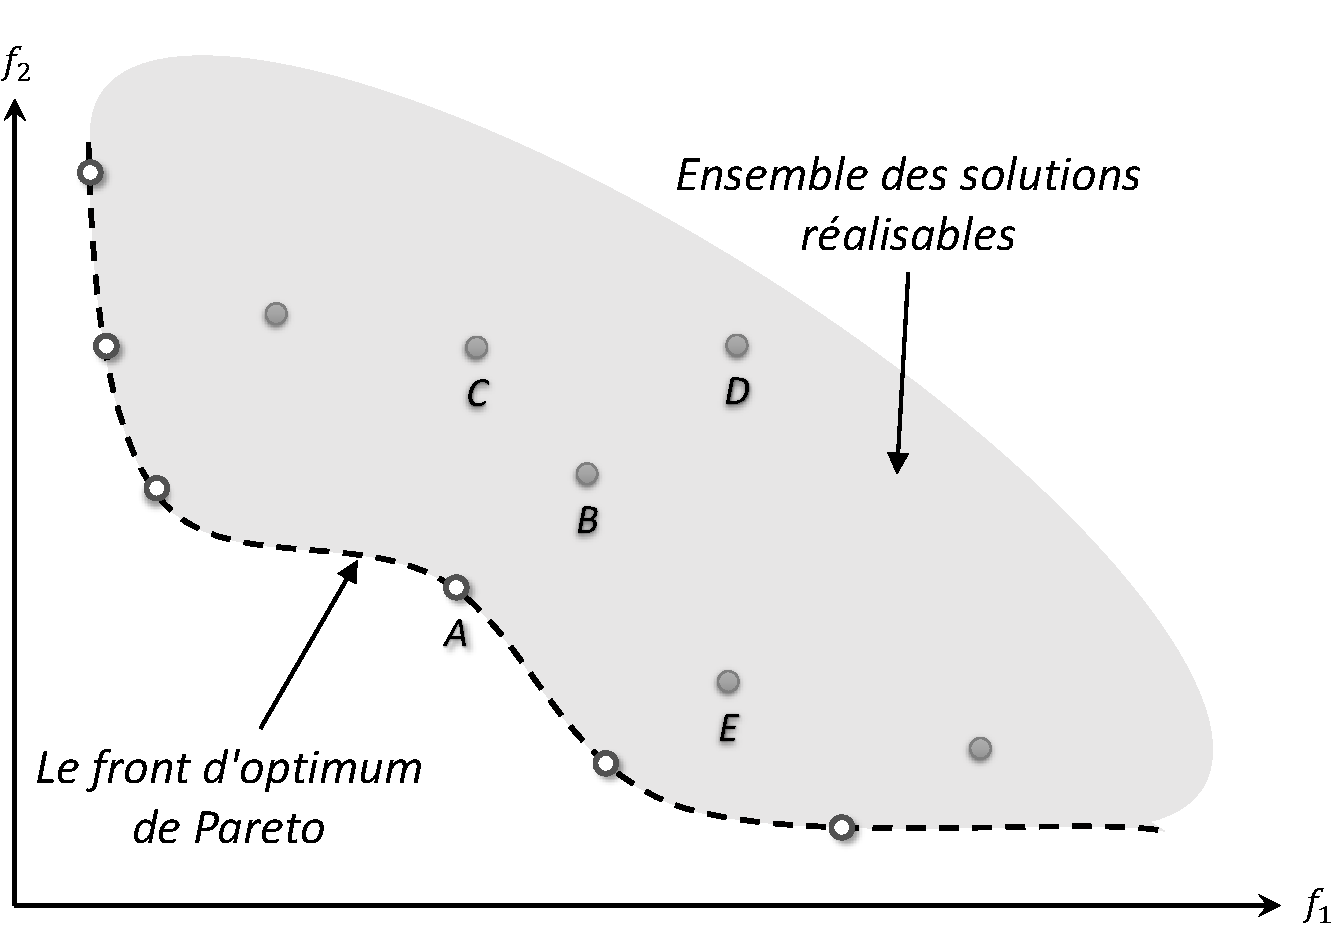
\includegraphics[scale=0.33]{chapitre2/chap2Fig/pareto-optimality.pdf}
  }
  \quad
  \subfloat[Exemple des relations entre les solutions.\label{fig:pareto-solutions}]{
    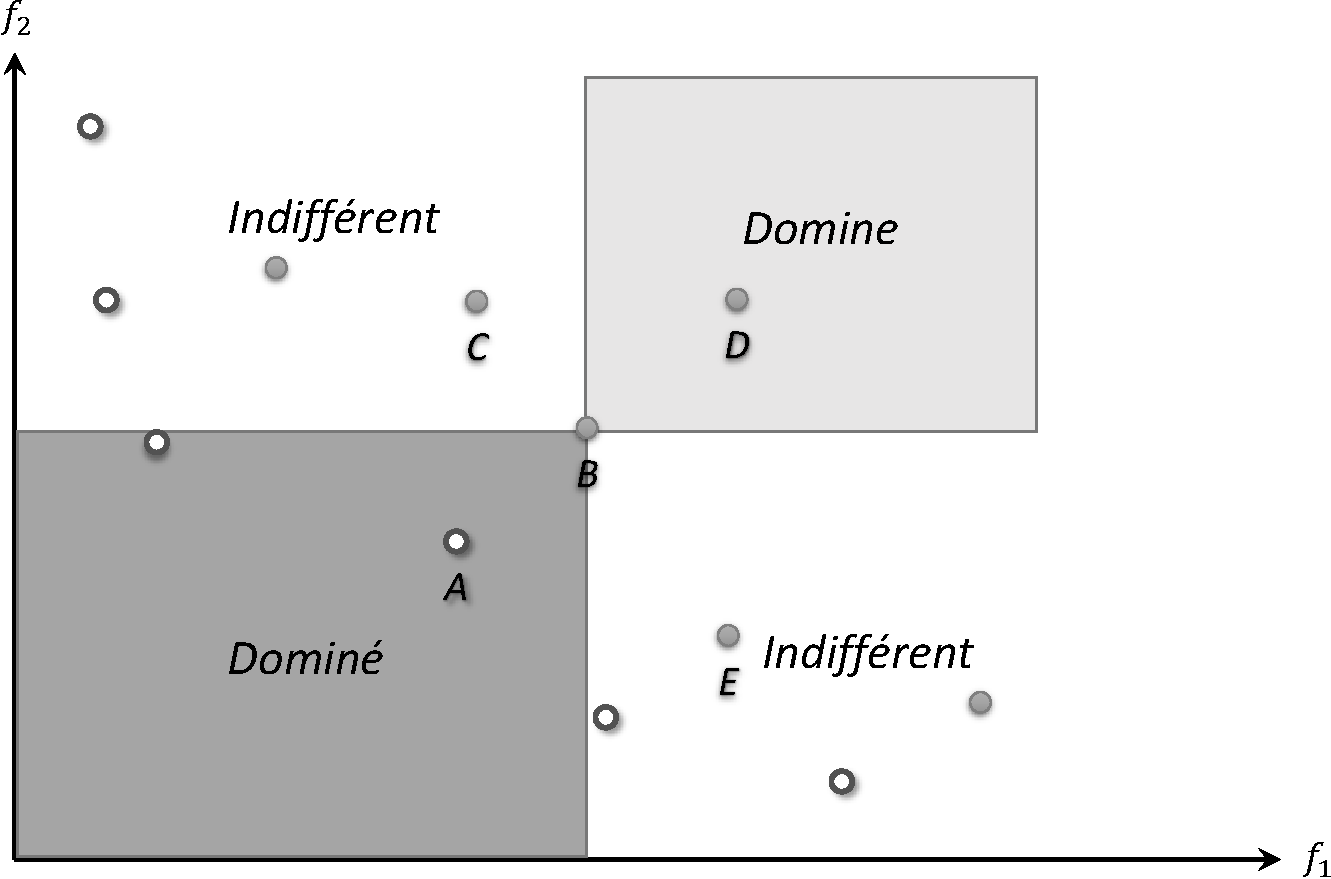
\includegraphics[scale=0.33]{chapitre2/chap2Fig/pareto-solutions.pdf}
  }
  \caption{Exemples de la notion de dominance de Pareto dans l'espace objectif.}\label{fig:pareto-optimality-example}
\end{figure}

Dans l'optimisation mono-objectif ($\mathcal{\acrshort[hyper=false]{OMO}}$), l'ensemble réalisable est totalement ordonné selon la fonction objectif $f$ : pour deux solutions $a$, $b \in X_f$ soit $f(a) \leqslant f(b)$ ou $f(b) \leqslant f(a)$. Le but est de trouver la ou les solutions qui donnent la valeur minimale de $f$ \cite{Deb01}. Cependant, lorsque plusieurs objectifs sont impliqués, la situation change : $X_f$ en général n'est pas totalement ordonné, mais partiellement ordonné. Ceci est illustré à la \ref{fig:pareto-optimality}. La solution représentée par le point $B$ est meilleure que la solution représentée par le point $D$. Elle serait préférable si c'est un problème $\mathcal{OMO}$. En effet, dans le cas entre les points $C$ et $D$ : malgré que les $f_2$ sont égaux, $C$ obtient de meilleures valeurs dans $f_1$ que $D$. Pour exprimer mathématiquement cette situation, les relations $=$, $\leqslant$ et $<$ sont étendues aux vecteurs objectifs par analogie avec le cas $\mathcal{OMO}$. Pour deux vecteurs objectifs quelconques $u$ et $v$ :
\begin{alignat}{2}
& u = v         \quad && \Leftrightarrow \quad \forall i \in \{1,\cdots,k\} : u_i = v_i \nonumber \\
& u \leqslant v \quad && \Leftrightarrow \quad \forall i \in \{1,\cdots,k\} : u_i \leqslant v_i \nonumber \\
& u < v         \quad && \Leftrightarrow \quad u \leqslant v \wedge u \neq v 
\end{alignat}
En utilisant cette notion, on considère que $A < B$, $B < D$, et par conséquent, $A < D$. Cependant, en comparant $B$ et $E$ dans les deux fonctions objectives, aucune des solutions ne peut être considérée comme meilleure, puisque $B \nleqslant E$ et $E \nleqslant B$. Par conséquent, deux vecteurs de décision $a$, $b$ peuvent avoir trois possibilités avec $\mathcal{PMO}$ en ce qui concerne la relation $\leqslant$ (contrairement à deux possibilités avec $\mathcal{OMO}$) : $f(a) \leqslant f(b)$, $f(b) \leqslant f(a)$ ou $f(a) \nleqslant f(b) \wedge f(b) \nleqslant f(a)$. Les notions suivantes sont utilisées pour classer les différentes situations.
\begin{definition}
 (\textit{Dominance de Pareto}) Pour deux vecteurs de décision quelconques $a$ et $b$,
 \begin{alignat}{2}
  & a \prec b        \; \text{($a$ domine $b$)}          \quad && \Leftrightarrow \quad f(a) < f(b) \nonumber \\
  & a \preccurlyeq b \; \text{($a$ domine faiblement $b$)} \quad && \Leftrightarrow \quad f(a) \leqslant f(b) \nonumber \\
  & a \sim b         \; \text{($a$ est indifférent à $b$)} \quad && \Leftrightarrow \quad f(a) \nleqslant f(b) \wedge f(b) \nleqslant f(a) 
  \end{alignat}
\end{definition}

Dans la \ref{fig:pareto-solutions}, le rectangle gris clair encapsule la région dans l'espace objectif qui est \textit{dominée} par le vecteur de décision représenté par $B$. Le rectangle gris foncé contient les vecteurs objectifs dont les vecteurs de décision correspondant \textit{dominent} la solution associée à $B$. Toutes les solutions pour lesquelles le vecteur objectif résultant n'est dans aucun rectangle sont \textit{indifférentes} à la solution représentée par $B$.

Sur la base du concept de dominance de Pareto, le \textit{critère d'optimalité} pour les $\mathcal{PMO}$ peut être introduit. Toujours en référence à la \ref{fig:pareto-solutions}, $A$ est unique parmi $B$, $C$, $D$ et $E$ : son vecteur de décision $a$ correspondant n'est pas dominé par aucun autre vecteur de décision. Cela signifie que $a$ est optimal dans le sens où il ne peut pas être amélioré dans une objective sans causer une dégradation dans au moins une autre objective. Ces solutions sont appelées \textit{optimum de Pareto} \cite{Branke08}.

\begin{definition}
(\textit{Optimalité de Pareto}) On dit qu'un vecteur de décision $x \in X_f$ est non-dominé pour un ensemble $A \subseteq X_f$ si et seulement si :
\begin{equation}
\nexists \; a \in A: a \prec x
\end{equation} 
En outre, $x$ est dit \textit{optimum de Pareto} si et seulement si $x$ est non-dominé pour $X_f$.
\end{definition}
Dans la \ref{fig:pareto-solutions}, les points blancs représentent des solutions optimales de Pareto. Ils sont indifférents les uns aux autres. Cela rend la principale différence à la $\mathcal{OMO}$ clair : il n'existe pas de solution optimale unique, mais plutôt un ensemble de compromis optimaux. Aucune solution d'entre elles ne peut être identifiée comme meilleure que les autres à moins que l'information de préférence soit incluse (par exemple, un classement des objectifs).

L'ensemble de toutes les solutions optimales de Pareto est appelé \textit{ensemble d'optimum de Pareto}; Les vecteurs objectifs correspondants forment \textit{le front ou la surface d'optimum de Pareto} \cite{Deb01}.

\begin{figure}
\begin{center}
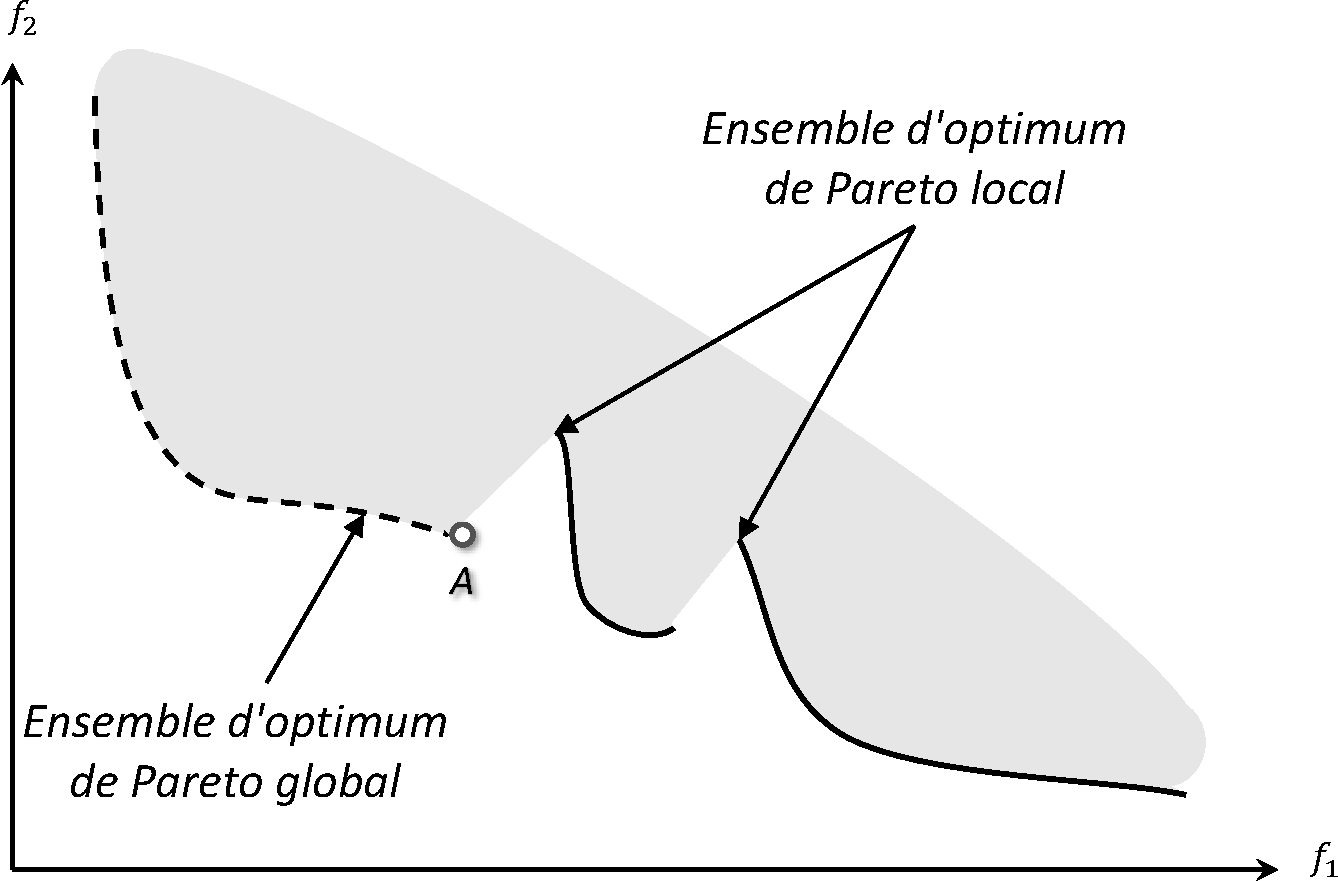
\includegraphics[scale=0.4]{chapitre2/chap2Fig/pareto-global-local.pdf}
\caption{Exemple d'ensembles de solutions localement optimales et de solutions globalement optimales dans l'espace objectif.}
 \label{fig:pareto-global-local}
\end{center}
\end{figure}

\begin{definition}
 (\textit{Ensembles et fronts non dominés}) Soit $A \subseteq X_f$. La fonction $p(A)$ donne l'ensemble des vecteurs de décision non dominés en $A$ :
 \begin{equation}
  P(A) = \{a \in A | a \text{ est non-dominé sur } A\}
 \end{equation}
 $p(A)$ est l'ensemble non-dominé sur $A$, l'ensemble correspondant de vecteurs objectifs $f(p(A))$ est le front non-dominé de $A$. En outre, $X_p = p(X_f)$ est nommé l'ensemble d'optimum de Pareto et $Y_p = f (X_p)$ est désigné comme le front d'optimum de Pareto.
\end{definition}

L'ensemble d'optimum de Pareto comprend les solutions globalement optimales. Cependant, il peut y avoir des optima locaux qui constituent un ensemble non-dominé dans un certain voisinage. Ceci correspond aux concepts des ensembles d'optimum de Pareto globaux et locaux \cite{Deb01} :

\begin{definition}
 Considérons un ensemble de vecteurs de décision $A \subseteq X_f$.
 L'ensemble $A$ est nommé comme un ensemble d'optimum de Pareto local si et seulement si :
 \begin{equation}
  \forall a \in A: \nexists x \in X_f : x \prec a \wedge ||x - a|| < \epsilon \wedge ||f(x) - f(a) || < \delta
 \end{equation}
 Où $|| . ||$ est une métrique de distance correspondante et $ \epsilon > 0$, $ \delta > 0$.
 L'ensemble $A$ est appelé ensemble d'optimum de Pareto global si et seulement si :
 \begin{equation}
  \forall a \in A: \nexists x \in X_f : x \prec a
 \end{equation}
\end{definition}
La différence entre optimum local et global est visualisée dans la \ref{fig:pareto-global-local}. La ligne pointillée constitue un front d'optimum de Pareto global, alors que la ligne continue représente un front d'optimum de Pareto local. Enfin, notez qu'un ensemble d'optimum de Pareto global ne contient pas nécessairement toutes les solutions d'optimum de Pareto et que tout ensemble d'optimum de Pareto global est aussi un ensemble d'optimum de Pareto local.

\subsection{Méthodes de résolution}
En résolvant un $\mathcal{PMO}$, deux types de problèmes peuvent être identifiés \cite{Branke08} : (1) la \textit{recherche} et (1) la \textit{prise de décision}. Le premier aspect concerne le processus d'optimisation dans lequel l'ensemble des solutions réalisable est échantillonné pour trouver les solutions d'optimum de Pareto. Le second aspect traite le problème de sélection d'une solution de compromis appropriée à partir de l'ensemble d'optimum de Pareto. Un décideur humain est nécessaire pour faire le compromis, souvent difficile, entre les objectifs contradictoires.

Suivant la combinaison du processus d'optimisation et la prise de décision, les méthodes d'optimisation multi-objectifs peuvent être classées en trois catégories \cite{Hwang79,Marler04,Collette13} :
\begin{itemize}
 \item \textbf{Méthodes a priori.} Prise de décision \textit{avant} la recherche : Les fonctions objectifs du $\mathcal{PMO}$ sont regroupées en une seule objectif qui inclut implicitement les informations de compromis fournies par le décideur.
 \item \textbf{Méthodes interactives.} Prise de décision \textit{durant} la recherche : Le décideur peut donner ses préférences de compromis au cours du processus d'optimisation d'une manière interactive. Après chaque étape d'optimisation, un certain nombre de compromis alternatifs sont présentés aux décideur, sur la base desquels il spécifie une autre information de préférence, qui guide respectivement la recherche.
 \item \textbf{Méthodes a posteriori.} Prise de décision \textit{après} la recherche : L'optimisation est effectuée sans aucune préférence donnée. Le résultat du processus de recherche est un ensemble de solutions candidates (d'optimum de Pareto) dont le choix final de la meilleure solution est fait par le décideur.
\end{itemize}

Les méthodes de différentes classes ont leurs avantages et inconvénients et, pour cette raison, différentes approches sont nécessaires pour résoudre un $\mathcal{PMO}$. Signalons que la classification donnée ici n'est pas complète ou absolue. Le chevauchement et les combinaisons d'approches sont possibles et certaines méthodes peuvent appartenir à plusieurs classes en fonction de différentes interprétations \cite{Branke08}. Cependant, nous allons utiliser la classification proposée par \textit{Deb} \cite{Deb01}, où les méthodes sont classées en deux catégories : (1) méthodes \textit{classiques} et (2) méthodes \textit{évolutionnaires}. Dans ce qui suite, nous présentons chacune des catégories.

\subsubsection{Méthodes classiques}
Les méthodes classiques pour résoudre le $\mathcal{PMO}$ regroupent les objectifs en une seule fonction objectif paramétrée. Il existe une panoplie de méthodes appartenant à cette classe, nous citons parmi elles : la méthode de pondération, la méthode $\epsilon$-contrainte, la méthode programmation par but, etc \cite{Collette13,Branke08,Deb01}.

\paragraph{Méthode de pondération}
Dans la méthode de pondération ou somme pondérée, le $\mathcal{PMO}$ original est convertie en un problème $\mathcal{OMO}$ en formant une combinaison linéaire des objectifs \cite{Gass55,Zadeh63} :
\begin{alignat}{2}
& \text{minimiser} \quad && y = f(x) = \sum_{i=1}^{k}\omega_i \cdot f_i(x) \nonumber \\
& \text{avec}   \quad && x \in X_f
\end{alignat}
Les $\omega_i$ sont appelés poids et sont normalisés tels que $\sum \omega_i = 1$. Résoudre le problème d'optimisation ci-dessus pour un certain nombre de combinaisons de poids différentes donne un ensemble de solutions. A condition que tous les poids soient positifs, cette méthode produira uniquement des solutions d'optimum de Pareto.
La méthode de pondération peut être utilisée comme une méthode a posteriori de sorte que différents poids sont utilisés pour générer différentes solutions d'optimum de Pareto, et ensuite le décideur est invité à sélectionner la plus satisfaisante d'entre elles. Alternativement, le décideur peut être invité à spécifier les poids, dans ce cas la méthode est utilisée comme une méthode a priori.

\begin{example}
 La \ref{fig:weighted-sum-ex} illustre le fonctionnement de la méthode de pondération. Nous considérons le problème à deux objectifs. Avec deux objectifs, il existe deux poids $\omega_1$ et $\omega_2$, mais un seul est indépendant. Connaissant un, l'autre peut être calculé par une simple soustraction. Connaissant les poids, nous pouvons également calculer la fonction composite $f(x)$. Ses surfaces d'hyperplan (une droite) peuvent alors être visualisées dans l'espace objectif, comme le montrent les lignes << \textit{a} >>, << \textit{b} >>, << \textit{c} >> et << \textit{d} >> dans la \ref{fig:weighted-sum-ex}. Puisque notre problème nécessite une minimisation de $f(x)$, la tâche consiste à trouver l’hyperplan avec la valeur $f(x)$ minimale. Cela se produit avec l'hyperplan qui est tangent à l'espace de recherche et se trouve également dans le coin inférieur gauche de cet espace. Sur la figure, cette ligne est marquée comme << \textit{d} >>. Le point tangent $A$ est la solution minimale de $f(x)$ et est par conséquent la solution d'optimum de Pareto.
\end{example}

\begin{figure}
\begin{center}
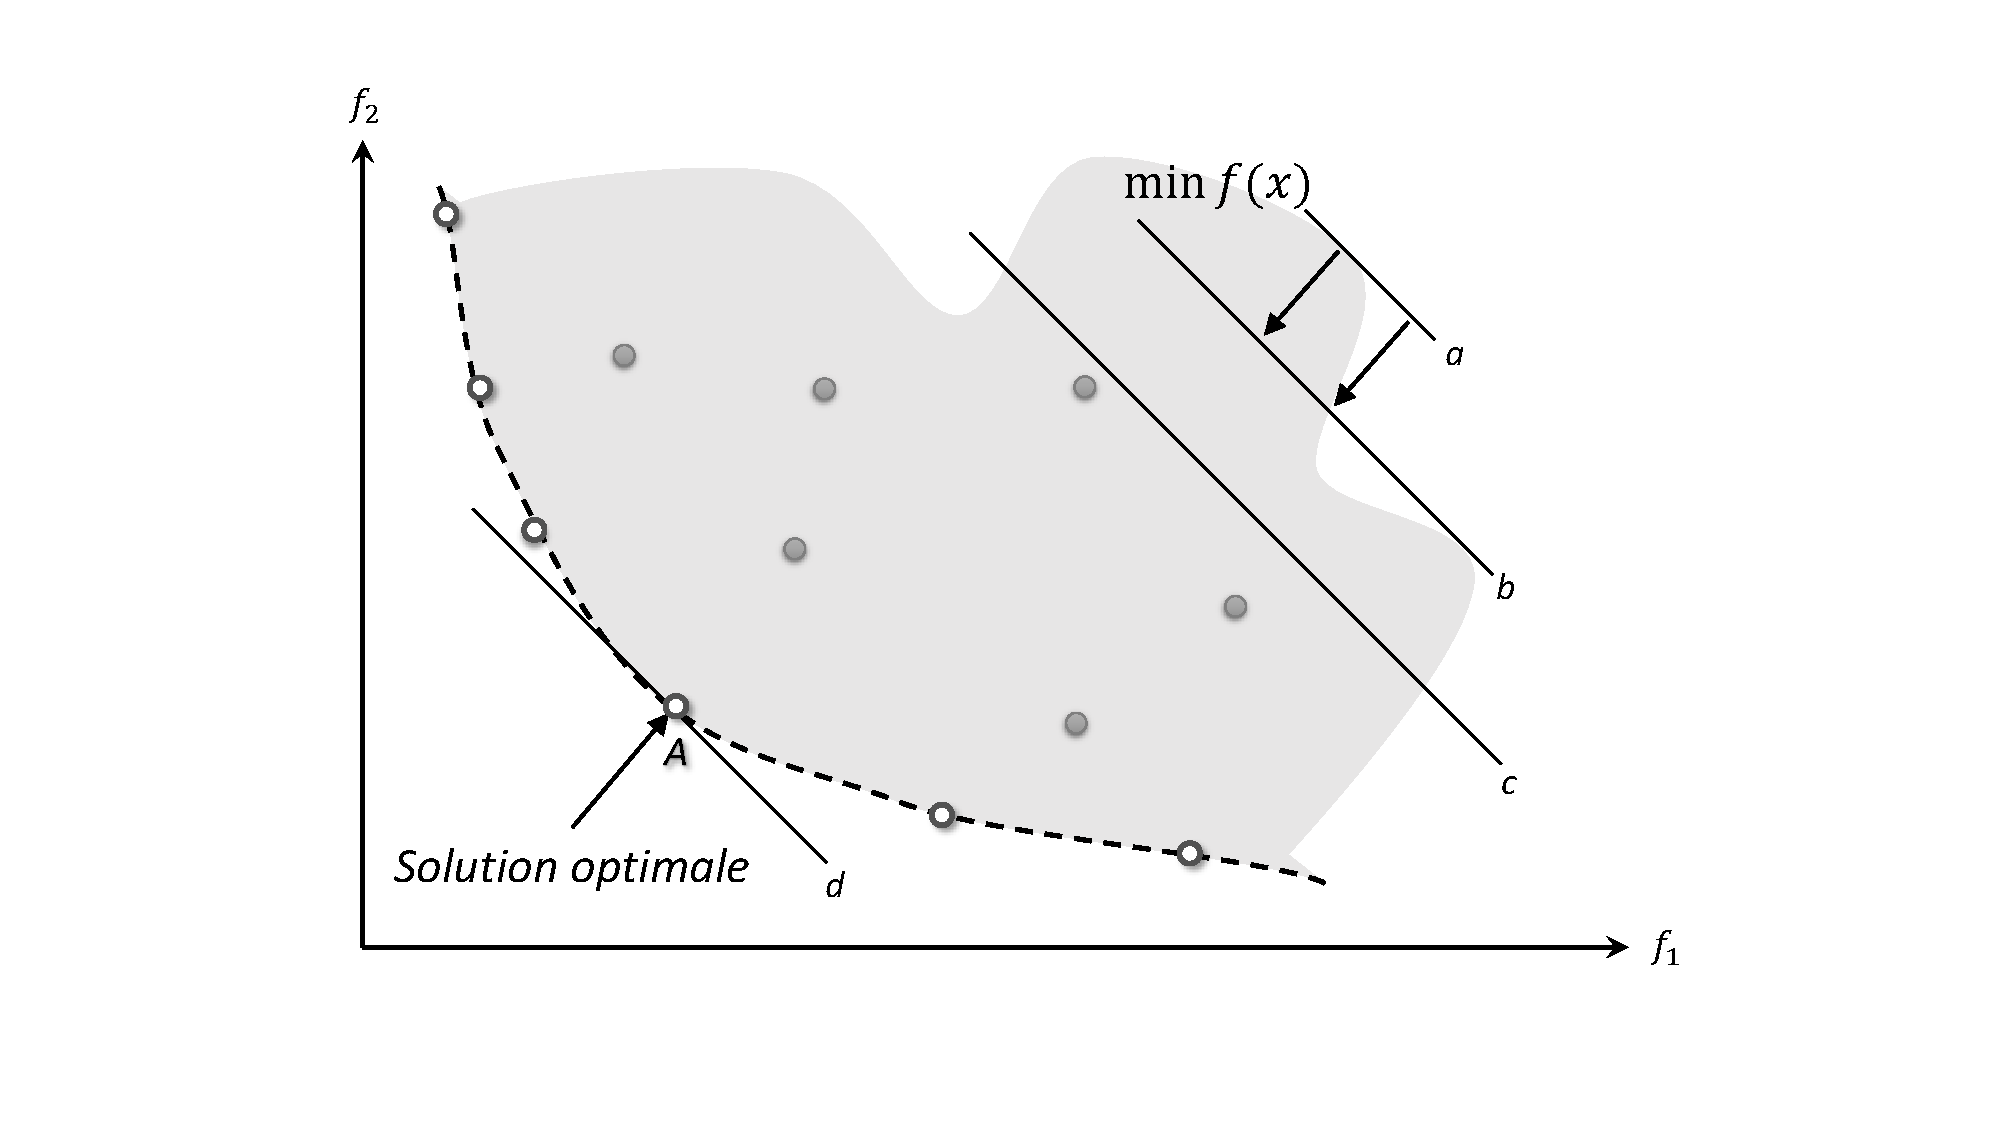
\includegraphics[scale=0.4]{chapitre2/chap2Fig/weighted-sum-ex.pdf}
\caption{Exemple de la méthode de pondération.}
 \label{fig:weighted-sum-ex}
\end{center}
\end{figure}

L’avantage de cette méthode est sa facilité d’implémentation et le fait qu’elle puisse être utilisée avec les méthodes et techniques définis pour $\mathcal{OMO}$. Cependant, comme mentionné précédemment, il est important dans $\mathcal{PMO}$ que les solutions d'optimum de Pareto soient générées et que toute solution puisse être trouvée. À cet égard, la méthode de pondération présente un sérieux défaut. La solution d'optimum de Pareto peut être trouvée en modifiant les poids seulement si le problème est convexe. Ainsi, il peut arriver que certaines solutions d'optimum de Pareto pour des problèmes non convexes ne puissent être trouvées, peu importe la façon dont les poids sont sélectionnés \cite{Branke08}. C'est le cas du point $A$ dans la \ref{fig:pareto-optimality}.


\paragraph{Méthode $\epsilon$-contrainte}
Afin d'atténuer les difficultés rencontrées par la méthode de somme pondérée dans la résolution de problèmes ayant des espaces objectifs non convexes, la méthode de $\epsilon$-contrainte est utilisée. L'idée de cette méthode est la transformation des $k-1$ fonctions objectives en contraintes. La fonction objective restante, qui peut être choisi arbitrairement, est la fonction objective du $\mathcal{OMO}$ résultant \cite{Haimes71,Vira83} :
\begin{alignat}{2}
& \text{minimiser} \quad && y = f(x) = f_h(x) \nonumber \\
& \text{avec}   \quad && e_i(x) = f_i(x) \leqslant \epsilon_i \quad (1 \leqslant i \leqslant k, i \neq h)  \nonumber \\
& \text{et}   \quad && x \in X_f
\end{alignat}
Les limites supérieures, $\epsilon_i$, sont les paramètres à varier afin de trouver des solutions d'optimum de Pareto. En pratique, il peut être difficile de spécifier les limites supérieures pour avoir des solutions aux problème $\mathcal{OMO}$, c'est-à-dire que la région réalisable ne soit pas vide. Cette difficulté est soulignée lorsque le nombre de fonctions objectives augmente \cite{Branke08}. Cependant, il est possible d'utiliser la méthode de manière a priori et demander au décideur de spécifier la fonction à optimiser et les limites supérieures.

\paragraph{Méthode programmation par but}
L'idée principale de la programmation par but est de trouver des solutions qui atteignent une cible prédéfinie pour une ou plusieurs fonctions objectives \cite{Charnes55}. Dans cette méthode, le décideur est invité à spécifier les niveaux cibles $z_i (i = 1, \cdots, k)$ pour les fonctions objectives. Ensuite, les écarts par rapport à ces niveaux cibles sont minimisés. Une fonction objective conjointement avec un niveau de cible est appelée un \textit{but}. Pour les problèmes de minimisation, les buts sont de la forme $f_i(x) \leqslant z_i$ et les niveaux de cibles sont supposés être sélectionnés. Après la formations des buts, les \textit{écarts} $\delta_i = max[0, f_i(x) - z_i]$ des valeurs de la fonction objective sont minimisés.

La méthode comporte plusieurs variantes. Dans l'approche de \textit{programmation par but pondérés} \cite{Charnes77}, la somme pondérée des écarts est minimisée. Cela signifie qu'en plus des niveaux de cibles, le décideur doit spécifier des poids positifs. Puis nous résolvons le problème :
\begin{alignat}{2}
& \text{minimiser} \quad && \sum_{i=1}^{k}\omega_i \delta_i \nonumber \\
& \text{avec}      \quad && f_i(x) - \delta_i \leqslant z_i \text{ et } \delta_i \geqslant 0  \nonumber \\
& \text{et}   \quad && x \in X_f
\end{alignat}

D'autre part, dans l'approche de \textit{programmation par but lexicographiques}, le décideur doit spécifier un ordre lexicographique pour les buts en plus des niveaux de cible. Après l'ordonnancement lexicographique, le problème des déviations en tant que fonctions objectives est résolu lexicographiquement \cite{Collette13}. Mentionnons également une approche de \textit{programmation par but min-max} où le maximum d'écarts est minimisé \cite{Deb01}.

\subsubsection{Méthodes évolutionnaires}
Les algorithmes évolutionnaires (\acrshort[hyper=false]{AE}) sont des méthodes de recherche inspirées de la nature pour résoudre des problèmes complexes avec un grand espace de recherche. Certaines caractéristiques de cette technique, tel que la possibilité de trouver des solutions optimales multiples dans une seule simulation, les rendent populaires et motivent les chercheurs à les utiliser dans divers domaines d'applications comme alternative aux méthodes classiques décrites précédemment.

Il existe plusieurs familles historiques d'algorithme évolutionnaires qui se sont développées de façon indépendante : la programmation évolutionnaire, les algorithmes génétiques, les stratégies d’évolutions et la programmation génétique.
Aujourd'hui, ces terminologies sont considérées comme sous-domaines des AE \cite{Branke08}.

Cette section vise à fournir un aperçu d'un certain nombre d'AE bien connus, conçus pour traiter des problèmes d'optimisation multi-objectifs, par la présentation du vocabulaire et le principe général de leurs fonctionnements.

\paragraph{Principe de fonctionnement}
En général, un AE se caractérise par trois faits :
\begin{enumerate}
 \item un ensemble de solutions candidates est maintenu, ce qui
 \item subit un processus de sélection, et qui
 \item est manipulé par les opérateurs génétiques, généralement le croisement et la mutation.
\end{enumerate}

Par analogie avec l'évolution naturelle, les solutions candidates sont appelées \textit{individus} et l'ensemble des solutions candidates s'appelle la \textit{population}. Chaque individu représente une solution possible, et il est codé sur la base d'une structure appropriée. Sans perte de généralité, on suppose que cette structure est un vecteur, par exemple un vecteur de bits ou un vecteur de valeur réelle. L'ensemble de tous les vecteurs possibles constitue \textit{l'espace des individus} $I$. Dans cette terminologie, la population est un ensemble de vecteurs $i \in I$.

Dans le processus de \textit{sélection}, qui peut être stochastique ou complètement déterministe, les individus de faible qualité sont retirés de la population, tandis que les individus de haute qualité sont reproduits. L'objectif est de concentrer la recherche sur des portions particulières de l'espace de recherche et d'augmenter la qualité moyenne au sein de la population. La qualité d'un individu par rapport à la tâche d'optimisation est représentée par une valeur scalaire, qui est le \textit{fitness}.

Le \textit{croisement} et la \textit{mutation} visent à générer de nouvelles solutions dans l'espace de recherche par la variation de celles existantes. L'opérateur de croisement prend un certain nombre de parents et crée un certain nombre d'enfants en recombinant les parents. Pour simuler la nature stochastique de l'évolution, une probabilité de croisement est associée à cet opérateur. En revanche, l'opérateur de mutation modifie les individus en changeant de petites parties dans les vecteurs associés selon un taux de mutation donné. L'opérateur de \textit{l'élitisme} assure que la nouvelle population garde que les meilleures solutions de la population actuelle.

Sur la base des concepts ci-dessus, l'évolution naturelle est simulée par un processus itératif de calcul. Premièrement, une population initiale est créée au hasard ou suivant un schéma. Ensuite, une boucle (\textit{génération}) comprenant les étapes : évaluation (affectation de fitness), sélection, croisement et/ou mutation est exécutée un certain nombre de fois fixé. À la fin, le meilleur individu(s) dans la population finale, ou trouvé pendant tout le processus d'évolution, est le résultat de l'AE.

\begin{algorithm}
\caption{Algorithme général d'AE}
\label{algo:ae-algo}
\begin{algorithmic}[1]
\Require  $T$ \Comment{nombre maximal de générations}
\Ensure $A$ \Comment{ensemble non-dominé}
\State
$t = 0$;
\State
$Initialisation(P_t)$;
\Repeat
    \State $Evaluation(P_t)$;
    \State $P_t^\prime = Selection(P_t)$;
    \State $P_t^{\prime\prime} = Croisement(P_t^\prime)$;
    \State $P_{t+1} = Mutation(P_t^{\prime\prime})$;
	\State $t = t+1$;
\Until{$Termination(P_t, P_{t+1})$;}
\State
\Return $A$;
\end{algorithmic}
\end{algorithm}

Dans l'\ref{algo:ae-algo}, la procédure de base d'un AE est donnée. La population $P$ à une certaine génération $t$ est représentée par le symbole $P_t$.

%Cependant, nous discutons la deuxième catégorie des algorithmes qui sont supposés être plus rapides et meilleurs que les algorithmes non élitistes \cite{Deb01}.
Les AE multi-objectifs (\acrshort[hyper=false]{AEMO}) peuvent être classés généralement en trois approches basées sur : \textit{la dominance}, \textit{la décomposition} et \textit{les indicateurs} \cite{Wagner07}. Dans les sections suivantes, nous les détaillons et nous présentons un algorithme représentatif de chaque approche.

% 3.3.1 EMO Principles book: Introduction to Multiobjective Optimization: Interactive Approaches
% Figure 1.1 Basic Evolutionary Algorithm’s Flowchart
\paragraph{Approches basées sur la dominance}
Les méthodes de cette catégorie se base sur le concept de la dominance de Pareto déjà introduit. Ils sont les approches les plus populaires dans la littérature, et ils existent depuis les deux dernières décennies. Les AEMO de cette catégorie peuvent être classés en deux groupes principaux : des algorithmes \textit{non-élitistes} et des algorithmes \textit{élitistes}. Comme décrit précédemment, l'élitisme est un mécanisme pour préserver les bons individus de la génération actuelle en les sauvant et en les transmettant à la génération suivante, ce qui accélère la convergence de la population vers le front de Pareto. Le premier groupe inclue : \textit{Non-Dominated Sorting Genetic Algorithm} (NSGA) \cite{Srinivas94},
\textit{Niched-Pareto Genetic Algorithm} (NPGA) \cite{Horn94}, \textit{Multi-Objective Genetic Algorithm} (MOGA) \cite{Fonseca93}, etc. Le deuxième groupe comprend : \textit{Elitist Non-Dominated Sorting Genetic Algorithm} (\acrshort[hyper=false]{NSGA-II}) \cite{Deb02}, \textit{Strength Pareto Evolutionary Algorithm} (SPEA-II) \cite{Zitzler01} et \textit{Pareto Envelope-based Selection Algorithm} (PESA-II) \cite{Corne01}, et plusieurs autres algorithmes.

\subparagraph{NSGA-II}
Un exemple classique de cette catégorie est NSGA-II par Deb \textit{et al} \cite{Deb02}. Cet algorithme génétique utilise une méthode de \textit{ranking} qui attribue aux solutions non-dominées de la population courante le meilleur score. Par la suite, les solutions qui ne sont dominées que par les solutions potentiellement efficaces, reçoivent le second meilleur score et ainsi de suite. De cette manière, la population est organisée en couches où chaque couche contient des solutions non comparables entre elles. Le ranking d’une population est illustré dans la \ref{fig:nsgaii-rank}. Dans cet exemple, les solutions $A$, $B$, $C$, $D$ reçoivent le rang 1 car elles ne sont dominées par aucune solution. Les solutions $E$, $F$ et $G$ ont le rang 2 car elles ne sont dominées que par des solutions de rang 1. Enfin, $H$ et $I$ sont affectées au rang 3. NSGA-II utilise aussi une seconde mesure, la distance de \textit{crowding}, visant à améliorer la diversité de la population du premier rang de l’espace des objectifs. La distance de crowding est une mesure permettant de déterminer le surpeuplement des individus du même front. Il s'agit d'une estimation de la densité de solutions qui entourent un individu. Comme le montre la \ref{fig:nsgaii-crowd}, la distance de crowding $d_i$ pour l'individu $C$ est définie comme un demi-périmètre de cuboïde formé par les individus voisins les plus proches de $C$ dans l'espace objectif (les points $B$ et $D$).

\begin{figure}
  \centering
  \subfloat[La méthode de \textit{ranking}.\label{fig:nsgaii-rank}]{
    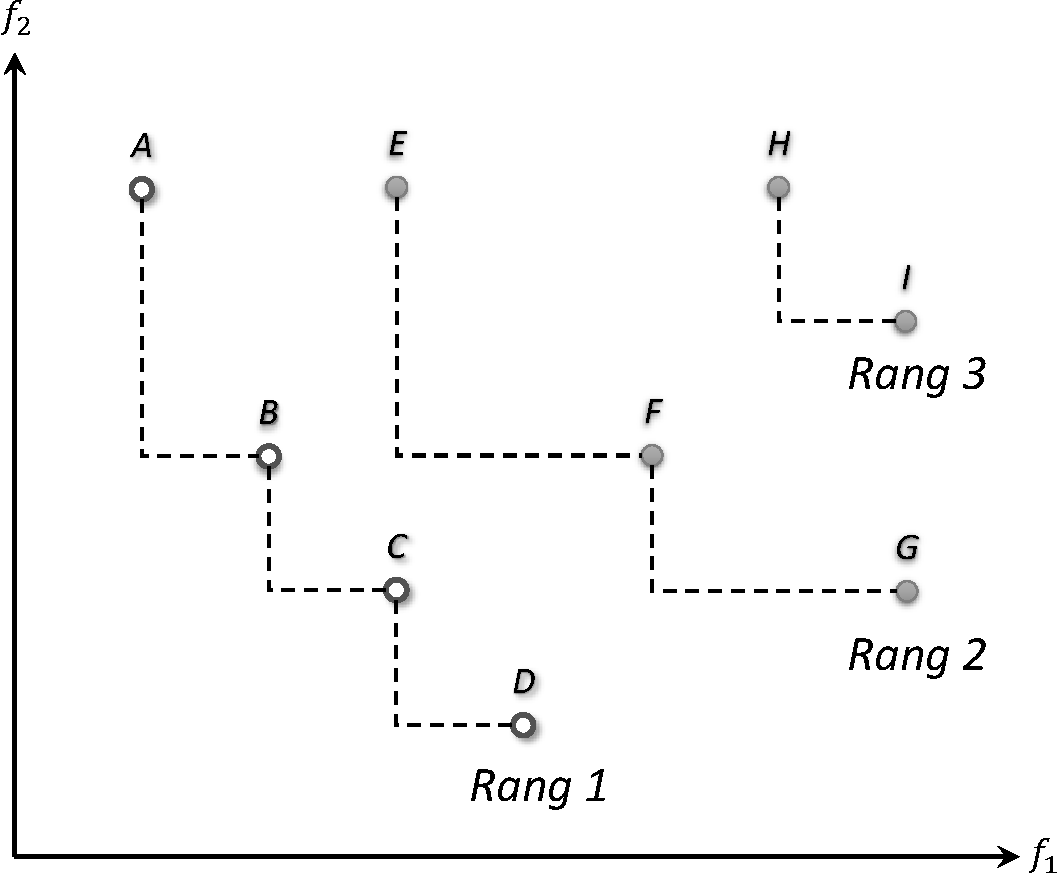
\includegraphics[scale=0.37]{chapitre2/chap2Fig/nsgaii-rank.pdf}
  }
  \quad
  \quad
  \subfloat[La méthode de la distance de \textit{crowding}.\label{fig:nsgaii-crowd}]{
    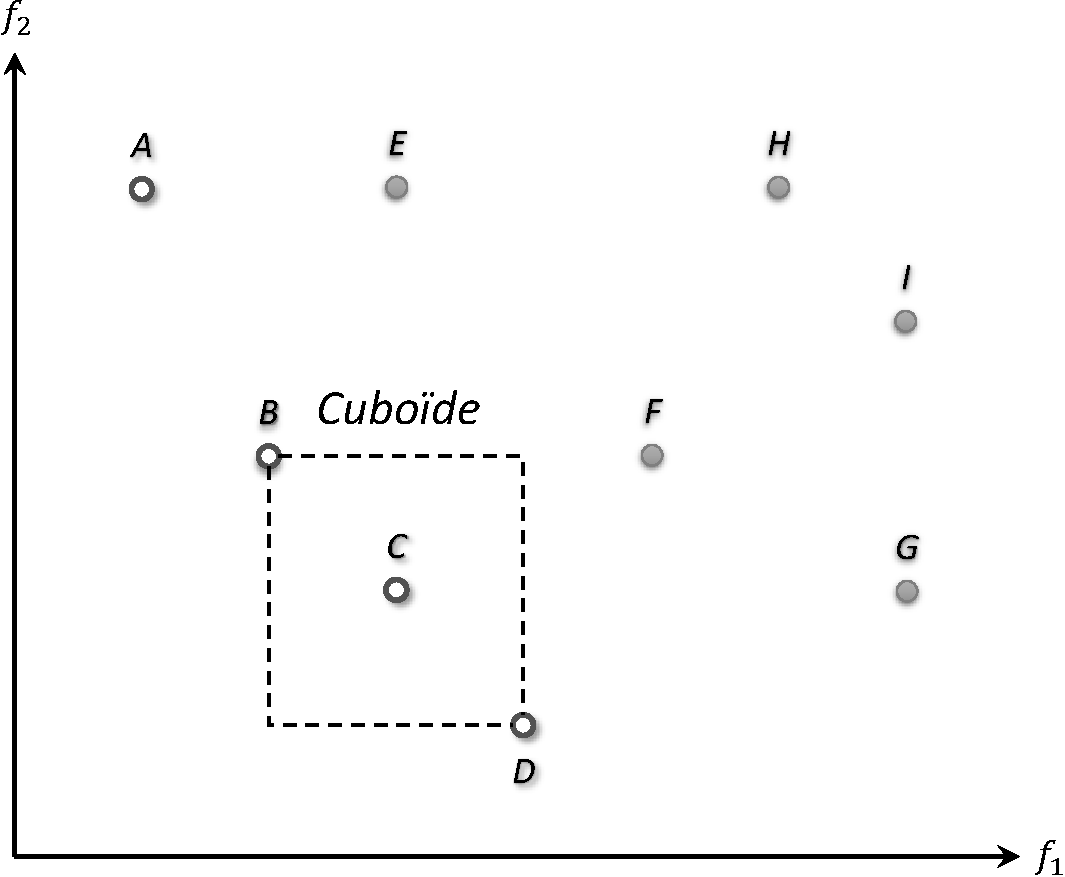
\includegraphics[scale=0.37]{chapitre2/chap2Fig/nsgaii-crowd.pdf}
  }
  \caption{Exemples des méthodes de NSGA-II.}\label{fig:nsgaii-example}
\end{figure}

\paragraph{Approches basées sur la décomposition}
Les méthodes basées sur la décomposition, connues aussi sous le nom d'approches d'agrégation pondérée, où un $\mathcal{PMO}$ est décomposé en un certain nombre de problèmes d'optimisation objectifs simples en utilisant un certain nombre de combinaisons de poids. Ces poids sont générés  soit de façon aléatoire \cite{Ishibuchi98}, soit dynamiquement et continuellement modifiées \cite{Jin01}, soit prédéfinies et uniformément réparties \cite{Murata01}. Parmi les algorithmes les plus courant : \textit{Multiple Single Objective Pareto Sampling} (MSOPS) \cite{Hughes03}, \textit{Multiobjective Evolutionary Algorithm based on Decomposition} (MOEA/D) \cite{Zhang07} et \textit{Repeated Single Objective} (RSO) \cite{Hughes05}.

\subparagraph{MOEA/D}
Cette variante récente d'algorithmes de décomposition a reçu une attention croissante en raison de sa simplicité de calcul et sa performance dans la recherche des solutions.
Le principe de cet algorithme est le suivant : Premièrement, il faut définir un $P$ vecteurs de poids uniformément distribués dans l’espace objectif. Ces vecteurs définissent des directions pour chercher les solutions. En effet, chaque vecteur de poids est utilisé pour définir un sous-problème mono-objectif en utilisant des fonctions scalaires comme la méthode de pondération ou la méthode de Tchebycheff. L’algorithme maintient également une population de solutions de taille $P$. Une solution est alors attachée à chaque fonction scalaire.

Le but de MOEA/D est de trouver les meilleures solutions par rapport à chacun des vecteurs de direction à l'aide de \textit{la notion de voisinage}. Étant donné un vecteur de direction $\lambda_i$ et le sous-problème scalaire sous-jacent pour tout $i \in \{1, \cdots, P\}$. L'algorithme définit l’ensemble $B(i)$ des voisins de $i$ comme étant les sous-problèmes correspondant aux vecteurs de direction les plus proches de $\lambda$. L’algorithme parcourt les sous-problèmes de façon itérative, et pour chacun, deux solutions parmi les voisins sont sélectionnées. Ces solutions permettent alors de produire une nouvelle solution, notée $y^\prime$, en utilisant des opérateurs de variations (mutation, croisement). La nouvelle solution $y^\prime$ est comparée aux solutions des voisins. Si $y^\prime$ permet d’améliorer la solution d’un voisin alors elle remplace cette solution et ainsi de suite pour tous les voisins. Ce mécanisme est répété pour toutes les directions jusqu’à ce qu’une condition d’arrêt soit satisfaite. A la fin, l’ensemble des solutions calculées par rapport à toutes ces directions est alors retourné en sortie.

\paragraph{Approches basées sur les indicateurs}
Une idée différente est d'attribuer un fitness aux individus basé sur un indicateur de performance pour évaluer la qualité, la convergence et la diversité des individus de la population. L'indicateur de \textit{l'hypervolume} \cite{Zitzler99b}, qui mesure le volume de la portion faiblement dominée par un ensemble de point dans l’espace objectif, a été largement adopté par les différents AEMO basés sur les indicateurs de performance. Cela est dû à sa précision et la diversité des ensembles de solutions non-dominées produits \cite{Wagner07}. Parmi les algorithmes proposés dans cette catégorie : \textit{Indicator-based Evolutionary Algorithm} (IBEA) \cite{Zitzler04} qui utilise une métrique de performance binaire comme indicateur, \textit{S-metric Selection-EMOA} (SMS-EMOA) \cite{Beume07} qui utilise l'indicateur d'hypervolume et plus récemment le \textit{Hypervolume Estimation Algorithm for Multiobjective Optimization} (HypE) \cite{Bader11} qui adopte la simulation Monte Carlo pour approximer la valeur exacte de l'hypervolume. Le principal défi de cette classe d'AEMO est la complexité élevée pour calculer l'indicateur de performance, en particulier lorsque le nombre d'objectifs est élevé \cite{Beume09}.

\subparagraph{IBEA}
L’idée principale de IBEA \cite{Zitzler04} est de formaliser les préférences entre individus en utilisant un indicateur de performance binaire de qualité $I$ arbitrairement choisi. Ensuite, chaque individu $x^1$ est attribué une valeur de fitness $F(x^1)$ correspondant à la mesure de la << perte en qualité >> si cet individu avait été retiré de la population $P$.
\begin{equation}
 F^\prime(x^1) = \sum_{x^2 \in P\setminus \{x^1\}} I(\{x^1\},\{x^2\})
\end{equation} 
Les auteurs proposent une autre formule modifiée qui amplifie l’influence des solutions non-dominées sur les solutions dominées. En d'autre terme, donner le plus grand score possible à une solution selon sa contribution par rapport aux autres solutions de la population.
\begin{equation}
 F(x^1) = \sum_{x^2 \in P\setminus \{x^1\}} - e^{-I(\{x^1\},\{x^2\})/k}
\end{equation}
Où $k > 0$ est un facteur d'échelle qui dépend de l’indicateur $I$ utilisé (par exemple, l'hypervolume ou epsilon) et du problème à optimiser.

\begin{figure}
\footnotesize
\begin{center}
\tikzset{
  basic/.style  = {draw, text width=4cm, drop shadow, rectangle},
  root/.style   = {basic, rounded corners=2pt, thin, align=center,
                   fill=green!30},
  level 2/.style = {basic, rounded corners=6pt, thin,align=center, fill=green!60,
                   text width=8em},
  level 3/.style = {basic, thin, align=left, fill=pink!60, text width=8.5em}
}

\begin{tikzpicture}[
  level 1/.style={basic,rounded corners=6pt, thin,align=center, fill=green!60,
                   text width=8em,sibling distance=97mm},
  level 2/.style = {basic, rounded corners=6pt, thin,align=center, fill=green!60,
                   text width=8em,sibling distance=50mm},
  level 3/.style = {basic, thin, align=left, fill=pink!60, text width=6.5em,sibling distance=40mm},
  edge from parent/.style={->,draw,black},
  >=latex]

% root of the the initial tree, level 1
\node[root] {Méthodes de résolution des $\mathcal{PMO}$}
% The first level, as children of the initial tree
  child {node[level 1] (c1) {Classiques}}
  child {node[level 1] (c2) {AEMO basés sur}
	  child {node[level 2,xshift=5pt] (c21) {La dominance}
		child {node[level 2,xshift=10pt] (c211) {Non-élitistes}}
		child {node[level 2,xshift=-10pt] (c212) {Élitistes}}
	  }
	  child {node[level 2] (c22) {La décomposition}}
	  child {node[level 2,xshift=-50pt] (c23) {Les indicateurs}}
  };

% The second level, relatively positioned nodes
\begin{scope}[every node/.style={level 3}]
\node [below of = c1, xshift=10pt, yshift=-5pt] (c11) {Pondération \cite{Gass55,Zadeh63}};
\node [below of = c11, yshift=-5pt] (c12) {$\epsilon$-contrainte \cite{Haimes71,Vira83}};
\node [below of = c12, yshift=-5pt] (c13) {Program. par but \cite{Charnes55,Charnes77}};

\node [below of = c211, xshift=10pt] (c2111) {NSGA \cite{Srinivas94}};
\node [below of = c2111] (c2112) {NPGA \cite{Horn94}};
\node [below of = c2112] (c2113) {MOGA \cite{Fonseca93}};

\node [below of = c212, xshift=10pt] (c2121) {NSGA-II \cite{Deb02}};
\node [below of = c2121] (c2122) {SPEA-II \cite{Zitzler01}};
\node [below of = c2122] (c2123) {PESA-II \cite{Corne01}};

\node [below of = c22, xshift=10pt] (c221) {MSOPS \cite{Hughes03}};
\node [below of = c221] (c222) {MOEA/D \cite{Zhang07}};
\node [below of = c222] (c223) {RSO \cite{Hughes05}};

\node [below of = c23, xshift=10pt] (c231) {IBEA \cite{Zitzler04}};
\node [below of = c231] (c232) {SMS-EMOA \cite{Beume07}};
\node [below of = c232] (c233) {HypE \cite{Bader11}};

\end{scope}

% lines from each level 1 node to every one of its "children"
\foreach \value in {1,...,3}
  \draw[->] (c1.178) |- (c1\value.west);

\foreach \value in {1,...,3}
  \draw[->] (c211.178) |- (c211\value.west);
  
\foreach \value in {1,...,3}
  \draw[->] (c212.178) |- (c212\value.west);
  
\foreach \value in {1,...,3}
  \draw[->] (c22.178) |- (c22\value.west);
  
\foreach \value in {1,...,3}
  \draw[->] (c23.178) |- (c23\value.west);
\end{tikzpicture}
\caption{Classification des méthodes de résolutions d'un $\mathcal{PMO}$.}
\label{fig:pmo-classification}
\end{center}
\end{figure}

La \ref{fig:pmo-classification} montre les différentes méthodes de résolution d'un $\mathcal{PMO}$ discutées dans cette section.

\subsection{Optimisation multi-objectifs dans les bases de données}
Nous passons maintenant sur l'application des techniques d'optimisation multi-objectifs décrites dans la section précédente dans le contexte des bases de données. En étudiant les travaux de littérature, nous trouvons que les techniques d'optimisation multi-objectifs ont été largement employées pour résoudre des problèmes diverses dans les base de données sur plusieurs niveaux : le Cloud Computing (ex: minimisation des coûts monétaire) \cite{Kong12,Dokeroglu14,Helff16}, les bases de données temps réel (ex: ordonnancement de requêtes) \cite{Thiele09,Zhao16}, la conception physique des bases de données (ex: le problème de sélection d'index \cite{Bruno11b,Bruno08}, la fragmentation \cite{Bellatreche13b,Bellatreche13c,Barr13}, les vues matérialisées \cite{Lawrence06,Talebian13,Goswami13}), le traitement de requête \cite{Papadimitriou01,Trummer14,Borzsony01}, etc.

Cependant, nous allons focaliser notre étude sur les vues matérialisées et la phase de traitement des requêtes par un SGBD.

\subsubsection{$\mathcal{PSV}$ multi-objectifs}
% 2.15 Multi-Objective View Selection Problem
% 3 papers: A Lexicographic Ordering Genetic Algorithm for Solving Multi-objective View Selection Problem
% Multiobjective Genetic Algorithms for Materialized View Selection in OLAP Data Warehouses
% Multiobjective Differential Evolution Algorithm Using Binary Encoded Data in Selecting Views for Materializing in Data Warehouse
Le $\mathcal{PSV}$ discuté dans le \ref{sec:psv} (ou une autre structure d'optimisation en général) peut être reformulé pour sélectionner un ensemble de vues avec plusieurs objectifs à optimiser en même temps. En effet, dans les travaux qui se basent sur l'optimisation mono-objectif, seul le coût de traitement de requête est considéré comme fonction objectif. Cependant, le coût de stockage ou de maintenance ont été considérés comme des contraintes à satisfaire.

En analysant les travaux de littérature, la première formalisation de $\mathcal{PSV}$ multi-objectif a été proposée dans \cite{Lawrence06}, dans lequel le temps de réponse de requête et le temps de maintenance doivent être minimisés simultanément sous la contrainte d'espace de stockage. La structure de représentation de données employée est la technique de cube treillis. Dans ce but, deux AEMO non-élitistes, MOGA et NPGA ont été adoptés pour résoudre le problème de sélection de vue. Pour faire face aux contraintes, l'auteur a proposé deux méthodes. La première méthode intègre la contrainte dans l'objectif et définit la notation de dominance de telle sorte qu'un individu infaisable est toujours dominé par un individu réalisable. La seconde permet à un individu infaisable d'être crée et d'utiliser une fonction de réparation pour le convertir en un faisable. Les résultats d'expérimentations sur des ensembles de données réelles et synthétiques montrent que les AEMO sont très compétitifs par rapport aux algorithmes de glouton classique.

Les auteurs de \cite{Talebian13} ont proposé un algorithme génétique basé sur le poids (WBGA) pour résoudre le problème de sélection de vue. L'objectif est de minimiser la somme pondérée du temps de réponse de requêtes et du temps de maintenance en fonction de la contrainte d'espace de stockage. Le cube treillis été utilisé comme structure de données. Le WBGA multiplie chaque objectif $i$ à un facteur de poids correspondant $w_i$ pour calculer une valeur de fitness. Contrairement à l'approche de la somme pondérée classique avec des poids fixes, la WBGA utilise le mécanisme d'optimisation génétique pour rechercher des solutions avec des poids différents en parallèle. Par conséquent, la population converge vers un ensemble de solutions optimales avec différents vecteurs de poids en un seul passage.

Dans \cite{Goswami13}, les auteurs ont mis en œuvre un algorithme à évolution différentielle (ED) multi-objectifs pour résoudre le $\mathcal{PSV}$ dans un entrepôt de données. Le temps de réponse et le coût de maintenance sont considérés comme fonctions objectifs, tandis que l'espace de stockage comme contrainte. Les solutions candidates sont représentées par la structure de MVPP. L'algorithme ED est une méthode méta-heuristiques stochastiques d'optimisation des espaces continus. La technique s'avère appropriée pour sélectionner des solutions représentatives à partir d'un grand nombre de solutions non-dominantes du $\mathcal{PSV}$.

% Approximation Schemes for Many-Objective Query Optimization
\subsubsection{Traitement de requêtes multi-objectifs}
Il existe souvent d'autres indicateurs de coûts en plus du temps d'exécution qui sont pertinents pour comparer les plans de requêtes, tel que le coût d'argent dans un scénario de Cloud Computing par exemple.
Les travaux qui implémentent les techniques d'optimisation multi-objectifs dans le contexte du traitement de requêtes peuvent être divisés en deux catégories. La première catégorie considère le niveau d'optimisation de requêtes, afin de produire des plans d'exécutions respectant les objectifs prédéfinis. D'autre part, la deuxième catégorie considère le niveaux données ou requêtage, en cherchant dans les données et produisant des résultats suivant les objectifs. Nous citons les travaux de chaque catégorie dans les sections suivantes.

\paragraph{Optimisation de requêtes}
L'optimisation de requêtes multi-objectifs modélise le coût d'un plan de requête comme un vecteur de coût où chaque composante vectorielle représente le coût selon une métrique de coût différente. L'optimisation classique des requêtes peut être considérée comme un cas particulier d'optimisation de requête multi-objectif où la dimension de l'espace de coût est égale à un (c'est-à-dire le nombre de composantes de vecteur de coût).

Différentes métriques de coût peuvent entrer en conflit. Par conséquent, l'objectif de l'optimisation est de trouver un plan de requête qui réalise le meilleur compromis entre les différentes métriques de coûts. Le meilleur compromis dépend des préférences de l'utilisateur fournies en entrée à l'optimiseur (par exemple, un utilisateur peut définir des pondérations entre différentes métriques de coûts pour exprimer une importance relative ou définir des bornes supérieurs/inférieurs de coût).

Le travail de \cite{Papadimitriou01} présente un algorithme d'approximation multi-objectifs pour exécuter des opérateurs d'une requête vers des sites dans le cas d'une base de données distribuée. Il suppose que chaque site soumet une << offre >> pour la requête, en spécifiant un délai pour la délivrance du résultat et un coût monétaire associé. L'optimiseur de requêtes compare alors ces offres à un compris entre le coût/délai fourni par l'utilisateur (une fonction $u(d)$, qui spécifie pour chaque valeur $d$ du délai, le montant d'argent que l'utilisateur est prêt à payer afin de recevoir les résultats de la requête dans le temps $d$) et tente de déterminer la combinaison des exécutions de la sous-requête qui maximise les préférences de l'utilisateur. Les auteurs proposent un algorithme glouton et une preuve mathématique pour résoudre ce problème.

Les auteurs de \cite{Fan06} ont proposé un framework de traitement des requêtes pour l'intégration des données. Ils considèrent la couverture, la densité et la latence des sources de donnée comme des fonctions objectives, et ils ont développé un modèle de coût pour estimer chacun d'entre eux.
Dans la phase d'optimisation, ils ont utilisé une méthode de pondération pour combiner les fonctions objectives en une seule fonction agrégée, en utilisant des paramètres de poids permettant à l'utilisateur de changer l'importance relative associée aux différents objectifs. Les expérimentations montrent que le modèle de coût est capable d'estimer efficacement chaque type d'objectif, et la procédure d'optimisation est capable de faire des compromis flexibles entre les objectifs lors du traitement des requêtes.

Les travaux récents de Trummer et Koch traitent le problème d'optimisation de requêtes ayant plusieurs objectifs (\textit{many-objective}). Grâce à l'avancement de la technologie de matériel informatique, les auteurs ont proposé de revisiter les suppositions faites par les chercheurs lors du développement des méthode d'optimisation de requêtes les premiers jours, afin d'exploiter les capacités logicielles et matérielles actuelles. Ils ont présenté le problème d'optimisation de requête multi-objectif où les plans de requêtes sont comparés selon plusieurs métriques de coût, comme par exemple le temps d'exécution, les frais monétaires, les mesures de consommation de ressources système (le nombre de noyaux utilisés, la quantité d'espace mémoire consommée). Les techniques utilisées pour résoudre ce problème inclues : des schémas d'approximation qui permettent de relaxer progressivement l'optimalité d'un plan pour accélérer le processus d'optimisation \cite{Trummer14b}, un algorithme incrémental qui divise l'optimisation en plusieurs petites étapes progressives, permettant aux utilisateurs de guider l'algorithme après chaque étape, ce qui rend de l'optimisation des requêtes un processus interactif \cite{Trummer15}, une optimisation de requêtes paramétrée, avec l'introduction d'une étape de pré-traitement si les requêtes correspondent à des modèles de requêtes connus à l'avance \cite{Trummer14}, une approche de décomposition qui permet de paralléliser l'optimisation de requêtes classique sur des clusters de grande taille avec des centaines de nœuds \cite{Trummer16}, l'utilisation d'un algorithme aléatoire (un Hill Climbing modifié) pour l'optimisation de requêtes multi-objectif qui est capable de traiter des requêtes avec des centaines de jointures \cite{Trummer16b}, la transformation du problème d'optimisation de requêtes en un programme linéaire en nombres entiers mixtes qui permet d'appliquer des solveurs de la programmation en nombres entiers pour traiter des espaces de recherche plus grands \cite{Trummer15b}, et enfin, ils ont présenté des résultats d'expérimentations pour résoudre le problème d'optimisation de requêtes sur l'ordinateur quantique D-Wave 2X avec plus de 1000 qubits (100 millions de fois plus rapide qu'un ordinateur classique) \cite{Trummer16c}.

\paragraph{L'opérateur Skyline}
L'opérateur Skyline est utilisé dans une requête et effectue un filtrage des résultats à partir d'une base de données afin qu'il ne conserve que les objets qui ne sont pas dominés par les autres.

Cet opérateur est une extension de SQL proposée par Börzsönyi \textit{et al.} \cite{Borzsony01}. Un exemple classique d'application de l'opérateur Skyline implique de choisir un hôtel pour des vacances. L'utilisateur veut que l'hôtel soit à la fois bon marché et proche de la plage. Cependant, les hôtels qui sont près de la plage peuvent également être coûteux. Dans ce cas, l'opérateur Skyline ne présenterait que les hôtels qui ne sont pas pires que tout autre hôtel à la fois dans le prix et la distance.
Dans le cas d'un ensemble de données composé d'objets multidimensionnels, un objet domine un autre objet s'il est aussi bon dans toutes les dimensions et mieux dans au moins une dimension \cite{Tiakas15}.

\begin{example}
 Börzsönyi \textit{et al.} ont proposé la syntaxe suivante pour l'opérateur Skyline \cite{Borzsony01} :
 %\begin{verbatim}
 \begin{lstlisting}[language=Sql]
  SELECT ... FROM ... WHERE ...
  GROUP BY ... HAVING ...
  SKYLINE OF [DISTINCT] d1 [MIN | MAX | DIFF],
                 ..., dm [MIN | MAX | DIFF]
  ORDER BY ...
 \end{lstlisting}
 %\end{verbatim}
 Où $d_1, \cdots d_m$ désignent les dimensions de Skyline et \texttt{MIN}, \texttt{MAX} et \texttt{DIFF} spécifient si la valeur de cette dimension doit être minimisée, maximisée ou simplement la différence.
\end{example}

L'opérateur Skyline peut être implémenté directement dans SQL en utilisant des instructions SQL courantes, mais cela s'est avéré être très lent \cite{Borzsony01}. D'autres algorithmes qui utilisent la méthode diviser pour régner, les indexes \cite{Borzsony01}, MapReduce \cite{Mullesgaard14} et calcul généraliste sur les cartes graphiques \cite{Bogh13} ont été proposés. Les requêtes Skyline sur les flux de données ont été étudiées dans le contexte du traitement parallèle des requêtes sur des systèmes multi-cœurs, en raison de leur large utilisation dans les problèmes de prise de décision en temps réel et les analyses de flux de données \cite{De16}.
Une étude récente et détaillée sur les différentes techniques d'implémentation du l'opérateur Skyline peut être trouvée dans \cite{Tiakas15}.

\subsection{Bilan et discussion}
Nous avons présenté dans cette section le problème de d'optimisation multi-objectifs, sa formulation et ses méthodes de résolution. Nous avons détaillé en particulier la méthode de la somme pondérée et les algorithmes NSGA-II, MOEA/D et IBEA car ils sont les plus populaires. De plus, nous avons cité les principaux travaux qui appliquent ce concept dans les bases de données, en particulier sur le problème de sélection de vues et le traitement de requêtes.

Dans notre étude, l'intégration du nouveau besoin non-fonctionnel qui est l'énergie dans la base de données, est considéré comme une fonction objective à optimiser. De ce fait, nous proposons de reformuler le problème de sélection des structures d'optimisations et le traitement de requête en un problème multi-objectifs, où il faut optimiser deux objectifs : le temps d'exécution de la charge de requêtes et la consommation d’énergie, avec la prise en compte des contraintes telles que le coût de maintenance et l'espace de stockage. Pour résoudre ce nouveau problème, il faut (1) proposer un modèle de coût qui permet de calculer la fonction objectif d'énergie, (2) adopter une méthode de prise de décision pour avoir un compromis entre la performance et l'énergie (une méthode a priori, interactive ou a posteriori), et (3) choisir la bonne configuration d'algorithme et des paramètres pour résoudre le $\mathcal{PMO}$.

\section{Conclusion}\label{sec:Conclusion}
Afin d'intégrer l'énergie dans une base de données, il faut, en premier lieu, l'étudier pour identifier ses composantes qui peuvent avoir un impact sur la consommation énergétique du système. Dans ce chapitre nous avons décrit l'ensemble des phases traditionnelles de cycle de vie de conception d’une base de données : l’analyse de besoins, la modélisation conceptuelle, logique, physique et le déploiement. Nous avons identifié l’opportunité d'intégrer l'énergie dans la phase de conception physique, plus précisément, dans le choix d'une structure d'optimisation. Nous nous sommes focalisés sur la technique redondante qui est les vues matérialisées, et nous avons proposé de reformuler le problème de sélection de vues en un problème multi-objectifs ou il faut minimiser le temps de réponse et la consommation d'énergie en respectant certaines contraintes. Nous avons également cité les travaux d'état de l'art qui traitement le $\mathcal{PSV}$ en version mono et multi-objectifs.

En seconde lieu, nous avons étudier la phase de traitement de requêtes dans un SGBD relationnel, qui inclue : la phase d'analyse, la transformation, la génération de plans et optimisation et enfin l'exécution. Cette étude nous a permis d'identifier les paramètres clés qu'il faut prendre en considération lors de conception d'un optimiseur de requêtes éco-énergétique. Ces paramètres incluent un modèle de coût pour estimer la consommation d'énergie d'une requête SQL et une technique d'intégration de ce modèle de coût dans la phase de génération de plans. En parallèle à la description des composantes d'un moteur de traitement de requête, nous avons passé en revue les principaux techniques et travaux proposés dans l'état de l'art.

En troisième lieu, nous avons focalisé notre attention sur les problèmes d'optimisation multi-objectifs. Car notre nouveau problème d'incorporation de l'énergie nécessite une reformulation multi-objectifs, afin de proposer aux utilisateurs et administrateurs de base de données un ensemble de solutions avec des compromis variés. Nous avons présenté la formulation des $\mathcal{PMO}$, ses principales méthodes de résolutions : classiques et évolutionnaires, et la démarche à suivre pour intégrer ces méthodes par rapport à l'utilisateur (méthode a priori, interactive ou a posteriori).

Dans le prochain chapitre, nous allons présenter le concept d'énergie, ses propriétés, et un état de l'art sur les travaux de minimisation d'énergie dans les systèmes informatiques.
